\documentclass[twoside]{book}

% Packages required by doxygen
\usepackage{fixltx2e}
\usepackage{calc}
\usepackage{doxygen}
\usepackage[export]{adjustbox} % also loads graphicx
\usepackage{graphicx}
\usepackage[utf8]{inputenc}
\usepackage{makeidx}
\usepackage{multicol}
\usepackage{multirow}
\PassOptionsToPackage{warn}{textcomp}
\usepackage{textcomp}
\usepackage[nointegrals]{wasysym}
\usepackage[table]{xcolor}

% NLS support packages
\usepackage[french]{babel}

% Font selection
\usepackage[T1]{fontenc}
\usepackage[scaled=.90]{helvet}
\usepackage{courier}
\usepackage{amssymb}
\usepackage{sectsty}
\renewcommand{\familydefault}{\sfdefault}
\allsectionsfont{%
  \fontseries{bc}\selectfont%
  \color{darkgray}%
}
\renewcommand{\DoxyLabelFont}{%
  \fontseries{bc}\selectfont%
  \color{darkgray}%
}
\newcommand{\+}{\discretionary{\mbox{\scriptsize$\hookleftarrow$}}{}{}}

% Page & text layout
\usepackage{geometry}
\geometry{%
  a4paper,%
  top=2.5cm,%
  bottom=2.5cm,%
  left=2.5cm,%
  right=2.5cm%
}
\tolerance=750
\hfuzz=15pt
\hbadness=750
\setlength{\emergencystretch}{15pt}
\setlength{\parindent}{0cm}
\setlength{\parskip}{3ex plus 2ex minus 2ex}
\makeatletter
\renewcommand{\paragraph}{%
  \@startsection{paragraph}{4}{0ex}{-1.0ex}{1.0ex}{%
    \normalfont\normalsize\bfseries\SS@parafont%
  }%
}
\renewcommand{\subparagraph}{%
  \@startsection{subparagraph}{5}{0ex}{-1.0ex}{1.0ex}{%
    \normalfont\normalsize\bfseries\SS@subparafont%
  }%
}
\makeatother

% Headers & footers
\usepackage{fancyhdr}
\pagestyle{fancyplain}
\fancyhead[LE]{\fancyplain{}{\bfseries\thepage}}
\fancyhead[CE]{\fancyplain{}{}}
\fancyhead[RE]{\fancyplain{}{\bfseries\leftmark}}
\fancyhead[LO]{\fancyplain{}{\bfseries\rightmark}}
\fancyhead[CO]{\fancyplain{}{}}
\fancyhead[RO]{\fancyplain{}{\bfseries\thepage}}
\fancyfoot[LE]{\fancyplain{}{}}
\fancyfoot[CE]{\fancyplain{}{}}
\fancyfoot[RE]{\fancyplain{}{\bfseries\scriptsize Généré par Doxygen }}
\fancyfoot[LO]{\fancyplain{}{\bfseries\scriptsize Généré par Doxygen }}
\fancyfoot[CO]{\fancyplain{}{}}
\fancyfoot[RO]{\fancyplain{}{}}
\renewcommand{\footrulewidth}{0.4pt}
\renewcommand{\chaptermark}[1]{%
  \markboth{#1}{}%
}
\renewcommand{\sectionmark}[1]{%
  \markright{\thesection\ #1}%
}

% Indices & bibliography
\usepackage{natbib}
\usepackage[titles]{tocloft}
\setcounter{tocdepth}{3}
\setcounter{secnumdepth}{5}
\makeindex

% Hyperlinks (required, but should be loaded last)
\usepackage{ifpdf}
\ifpdf
  \usepackage[pdftex,pagebackref=true]{hyperref}
\else
  \usepackage[ps2pdf,pagebackref=true]{hyperref}
\fi
\hypersetup{%
  colorlinks=true,%
  linkcolor=blue,%
  citecolor=blue,%
  unicode%
}

% Custom commands
\newcommand{\clearemptydoublepage}{%
  \newpage{\pagestyle{empty}\cleardoublepage}%
}

\usepackage{caption}
\captionsetup{labelsep=space,justification=centering,font={bf},singlelinecheck=off,skip=4pt,position=top}

%===== C O N T E N T S =====

\begin{document}

% Titlepage & ToC
\hypersetup{pageanchor=false,
             bookmarksnumbered=true,
             pdfencoding=unicode
            }
\pagenumbering{alph}
\begin{titlepage}
\vspace*{7cm}
\begin{center}%
{\Large Eclairage D\+IY S\+UP }\\
\vspace*{1cm}
{\large Généré par Doxygen 1.8.13}\\
\end{center}
\end{titlepage}
\clearemptydoublepage
\pagenumbering{roman}
\tableofcontents
\clearemptydoublepage
\pagenumbering{arabic}
\hypersetup{pageanchor=true}

%--- Begin generated contents ---
\chapter{Eclairage D\+IY S\+UP}
\label{index}\hypertarget{index}{}Projet de 2e année de B\+TS S\+N\+IR.



\section*{Présentation générale du système supportant le projet}

L’éclairage extérieur ouvre une vision sur le jardin en chassant les zones d’ombre, permet de mener des activités le soir sur la terrasse ou la pelouse \+: lire, faire des grillades au barbecue, prendre un repas, jouer aux cartes ou au ping-\/pong. Il est également utile pour ranger ce qui traîne dans le jardin à la nuit tombée, chercher un objet égaré, rentrer la voiture dans le garage ou mettre la clé dans la serrure. Judicieusement réparti dans le jardin, l’éclairage (blanc, unicolore ou multicolore) s’intègre dans le décor et crée une belle atmosphère nocturne en sculptant les volumes comme le démontre la figure 1. Implanté ponctuellement, il met en scène un arbre, un massif, un plan d’eau, une pergola, une particularité architecturale de la maison, une statue ou une jolie allée pavée.~\newline
 Un luminaire extérieur facilite les déplacements et limite les risques de chutes en signalant un escalier, une dénivellation ou le franchissement de sols différents, du gazon à la terrasse. Il balise une allée sinueuse, facilite la sortie des poubelles ou le franchissement du portail. Il possède également un effet dissuasif vis-\/à-\/vis des visiteurs indélicats en simulant la présence des propriétaires.

\section*{Objectif du candidat}

Vous développez le module \textquotesingle{}\hyperlink{classSUP}{S\+UP}\textquotesingle{} (Supervision des éclairages).~\newline
 Vous devez \+:~\newline
 – Développer une application W\+EB pour gérer (ajout, modification, suppression, configuration, activation, cycle) les éclairages~\newline
 – Mettre en place l’authentification d’accès à l’application W\+EB~\newline
 – Configurer via T\+C\+P/\+IP les éclairages multicolores~\newline
 – Mettre à jour les configurations des éclairages multicolores à partir des données reçue~\newline
 des contrôleurs~\newline
 – Enregistrer dans une base de données les configurations des éclairages multicolores~\newline
 – Mettre à jour l’application des éclairages multicolores~\newline
 – Commander, à distance, les éclairages~\newline
 – Exporter dans un fichier au format csv des configurations des éclairages~\newline
 – Importer à partir d’un fichier au format csv des configurations des éclairages~\newline
 
\chapter{Index hiérarchique}
\section{Hiérarchie des classes}
Cette liste d\textquotesingle{}héritage est classée approximativement par ordre alphabétique \+:\begin{DoxyCompactList}
\item \contentsline{section}{io\+:\+:detail\+:\+:Asynchronous\+Reader}{\pageref{classio_1_1detail_1_1AsynchronousReader}}{}
\item \contentsline{section}{io\+:\+:Byte\+Source\+Base}{\pageref{classio_1_1ByteSourceBase}}{}
\begin{DoxyCompactList}
\item \contentsline{section}{io\+:\+:detail\+:\+:Non\+Owning\+I\+Stream\+Byte\+Source}{\pageref{classio_1_1detail_1_1NonOwningIStreamByteSource}}{}
\item \contentsline{section}{io\+:\+:detail\+:\+:Non\+Owning\+String\+Byte\+Source}{\pageref{classio_1_1detail_1_1NonOwningStringByteSource}}{}
\item \contentsline{section}{io\+:\+:detail\+:\+:Owning\+Std\+I\+O\+Byte\+Source\+Base}{\pageref{classio_1_1detail_1_1OwningStdIOByteSourceBase}}{}
\end{DoxyCompactList}
\item \contentsline{section}{Client\+Tcp\+Com\+Bny}{\pageref{classClientTcpComBny}}{}
\item \contentsline{section}{Eclairage\+:\+:Controleur}{\pageref{classEclairage_1_1Controleur}}{}
\begin{DoxyCompactList}
\item \contentsline{section}{Eclairage\+Multicolore\+:\+:Controleur}{\pageref{classEclairageMulticolore_1_1Controleur}}{}
\item \contentsline{section}{Eclairage\+Unicolore\+:\+:Controleur}{\pageref{classEclairageUnicolore_1_1Controleur}}{}
\end{DoxyCompactList}
\item \contentsline{section}{io\+:\+:C\+S\+V\+Reader$<$ column\+\_\+count, trim\+\_\+policy, quote\+\_\+policy, overflow\+\_\+policy, comment\+\_\+policy $>$}{\pageref{classio_1_1CSVReader}}{}
\item \contentsline{section}{io\+:\+:double\+\_\+quote\+\_\+escape$<$ sep, quote $>$}{\pageref{structio_1_1double__quote__escape}}{}
\item \contentsline{section}{Eclairage}{\pageref{classEclairage}}{}
\begin{DoxyCompactList}
\item \contentsline{section}{Eclairage\+Multicolore}{\pageref{classEclairageMulticolore}}{}
\item \contentsline{section}{Eclairage\+Unicolore}{\pageref{classEclairageUnicolore}}{}
\end{DoxyCompactList}
\item \contentsline{section}{Eclairage\+Multicolore\+:\+:Eclairage\+Com\+Bny}{\pageref{classEclairageMulticolore_1_1EclairageComBny}}{}
\item \contentsline{section}{Eclairage\+Unicolore\+:\+:Eclairage\+Com\+Bny}{\pageref{classEclairageUnicolore_1_1EclairageComBny}}{}
\item \contentsline{section}{io\+:\+:empty\+\_\+line\+\_\+comment}{\pageref{structio_1_1empty__line__comment}}{}
\item \contentsline{section}{Eclairage\+:\+:Ent}{\pageref{classEclairage_1_1Ent}}{}
\begin{DoxyCompactList}
\item \contentsline{section}{Eclairage\+Multicolore\+:\+:Ent}{\pageref{classEclairageMulticolore_1_1Ent}}{}
\item \contentsline{section}{Eclairage\+Unicolore\+:\+:Ent}{\pageref{classEclairageUnicolore_1_1Ent}}{}
\end{DoxyCompactList}
\item std\+:\+:exception\begin{DoxyCompactList}
\item \contentsline{section}{io\+:\+:error\+:\+:base}{\pageref{structio_1_1error_1_1base}}{}
\begin{DoxyCompactList}
\item \contentsline{section}{io\+:\+:error\+:\+:can\+\_\+not\+\_\+open\+\_\+file}{\pageref{structio_1_1error_1_1can__not__open__file}}{}
\item \contentsline{section}{io\+:\+:error\+:\+:duplicated\+\_\+column\+\_\+in\+\_\+header}{\pageref{structio_1_1error_1_1duplicated__column__in__header}}{}
\item \contentsline{section}{io\+:\+:error\+:\+:escaped\+\_\+string\+\_\+not\+\_\+closed}{\pageref{structio_1_1error_1_1escaped__string__not__closed}}{}
\item \contentsline{section}{io\+:\+:error\+:\+:extra\+\_\+column\+\_\+in\+\_\+header}{\pageref{structio_1_1error_1_1extra__column__in__header}}{}
\item \contentsline{section}{io\+:\+:error\+:\+:header\+\_\+missing}{\pageref{structio_1_1error_1_1header__missing}}{}
\item \contentsline{section}{io\+:\+:error\+:\+:integer\+\_\+must\+\_\+be\+\_\+positive}{\pageref{structio_1_1error_1_1integer__must__be__positive}}{}
\item \contentsline{section}{io\+:\+:error\+:\+:integer\+\_\+overflow}{\pageref{structio_1_1error_1_1integer__overflow}}{}
\item \contentsline{section}{io\+:\+:error\+:\+:integer\+\_\+underflow}{\pageref{structio_1_1error_1_1integer__underflow}}{}
\item \contentsline{section}{io\+:\+:error\+:\+:invalid\+\_\+single\+\_\+character}{\pageref{structio_1_1error_1_1invalid__single__character}}{}
\item \contentsline{section}{io\+:\+:error\+:\+:line\+\_\+length\+\_\+limit\+\_\+exceeded}{\pageref{structio_1_1error_1_1line__length__limit__exceeded}}{}
\item \contentsline{section}{io\+:\+:error\+:\+:missing\+\_\+column\+\_\+in\+\_\+header}{\pageref{structio_1_1error_1_1missing__column__in__header}}{}
\item \contentsline{section}{io\+:\+:error\+:\+:no\+\_\+digit}{\pageref{structio_1_1error_1_1no__digit}}{}
\item \contentsline{section}{io\+:\+:error\+:\+:too\+\_\+few\+\_\+columns}{\pageref{structio_1_1error_1_1too__few__columns}}{}
\item \contentsline{section}{io\+:\+:error\+:\+:too\+\_\+many\+\_\+columns}{\pageref{structio_1_1error_1_1too__many__columns}}{}
\end{DoxyCompactList}
\item \contentsline{section}{Sqlite\+Persi\+Bny\+Exception}{\pageref{classSqlitePersiBnyException}}{}
\item \contentsline{section}{Tcp\+Ip\+Com\+Bny\+Exception}{\pageref{classTcpIpComBnyException}}{}
\end{DoxyCompactList}
\item \contentsline{section}{io\+:\+:ignore\+\_\+overflow}{\pageref{structio_1_1ignore__overflow}}{}
\item \contentsline{section}{Eclairage\+:\+:I\+H\+M\+Formulaire}{\pageref{classEclairage_1_1IHMFormulaire}}{}
\begin{DoxyCompactList}
\item \contentsline{section}{Eclairage\+Multicolore\+:\+:I\+H\+M\+Formulaire}{\pageref{classEclairageMulticolore_1_1IHMFormulaire}}{}
\item \contentsline{section}{Eclairage\+Unicolore\+:\+:I\+H\+M\+Formulaire}{\pageref{classEclairageUnicolore_1_1IHMFormulaire}}{}
\end{DoxyCompactList}
\item \contentsline{section}{Eclairage\+:\+:I\+H\+M\+Jardin}{\pageref{classEclairage_1_1IHMJardin}}{}
\begin{DoxyCompactList}
\item \contentsline{section}{Eclairage\+Multicolore\+:\+:I\+H\+M\+Jardin}{\pageref{classEclairageMulticolore_1_1IHMJardin}}{}
\item \contentsline{section}{Eclairage\+Unicolore\+:\+:I\+H\+M\+Jardin}{\pageref{classEclairageUnicolore_1_1IHMJardin}}{}
\end{DoxyCompactList}
\item \contentsline{section}{Eclairage\+Unicolore\+:\+:I\+H\+M\+Parametre}{\pageref{classEclairageUnicolore_1_1IHMParametre}}{}
\item \contentsline{section}{Eclairage\+Multicolore\+:\+:I\+H\+M\+Parametre}{\pageref{classEclairageMulticolore_1_1IHMParametre}}{}
\item std\+:\+:ios\+\_\+base\begin{DoxyCompactList}
\item std\+:\+:basic\+\_\+ios\begin{DoxyCompactList}
\item std\+:\+:basic\+\_\+istream\begin{DoxyCompactList}
\item std\+:\+:basic\+\_\+iostream\begin{DoxyCompactList}
\item std\+:\+:basic\+\_\+fstream\begin{DoxyCompactList}
\item std\+:\+:fstream\item \contentsline{section}{Fichier\+Texte\+Persi\+Bny}{\pageref{classFichierTextePersiBny}}{}
\end{DoxyCompactList}
\end{DoxyCompactList}
\end{DoxyCompactList}
\item std\+:\+:basic\+\_\+ostream\begin{DoxyCompactList}
\item std\+:\+:basic\+\_\+iostream\end{DoxyCompactList}
\end{DoxyCompactList}
\end{DoxyCompactList}
\item \contentsline{section}{io\+:\+:Line\+Reader}{\pageref{classio_1_1LineReader}}{}
\item \contentsline{section}{io\+:\+:no\+\_\+comment}{\pageref{structio_1_1no__comment}}{}
\item \contentsline{section}{io\+:\+:no\+\_\+quote\+\_\+escape$<$ sep $>$}{\pageref{structio_1_1no__quote__escape}}{}
\item \contentsline{section}{io\+:\+:set\+\_\+to\+\_\+max\+\_\+on\+\_\+overflow}{\pageref{structio_1_1set__to__max__on__overflow}}{}
\item \contentsline{section}{io\+:\+:single\+\_\+and\+\_\+empty\+\_\+line\+\_\+comment$<$ comment\+\_\+start\+\_\+char\+\_\+list $>$}{\pageref{structio_1_1single__and__empty__line__comment}}{}
\item \contentsline{section}{io\+:\+:single\+\_\+line\+\_\+comment$<$ comment\+\_\+start\+\_\+char\+\_\+list $>$}{\pageref{structio_1_1single__line__comment}}{}
\item \contentsline{section}{Sqlite\+Persi\+Bny}{\pageref{classSqlitePersiBny}}{}
\begin{DoxyCompactList}
\item \contentsline{section}{Eclairage\+:\+:Persi\+Bny}{\pageref{classEclairage_1_1PersiBny}}{}
\begin{DoxyCompactList}
\item \contentsline{section}{Eclairage\+Multicolore\+:\+:Persi\+Bny}{\pageref{classEclairageMulticolore_1_1PersiBny}}{}
\item \contentsline{section}{Eclairage\+Unicolore\+:\+:Persi\+Bny}{\pageref{classEclairageUnicolore_1_1PersiBny}}{}
\end{DoxyCompactList}
\end{DoxyCompactList}
\item \contentsline{section}{S\+UP}{\pageref{classSUP}}{}
\item \contentsline{section}{io\+:\+:detail\+:\+:Synchronous\+Reader}{\pageref{classio_1_1detail_1_1SynchronousReader}}{}
\item \contentsline{section}{Tcp\+Com\+Bny}{\pageref{classTcpComBny}}{}
\item \contentsline{section}{io\+:\+:throw\+\_\+on\+\_\+overflow}{\pageref{structio_1_1throw__on__overflow}}{}
\item \contentsline{section}{io\+:\+:trim\+\_\+chars$<$ trim\+\_\+char\+\_\+list $>$}{\pageref{structio_1_1trim__chars}}{}
\item \contentsline{section}{Uc\+Ajouter}{\pageref{classUcAjouter}}{}
\item \contentsline{section}{Uc\+Commander}{\pageref{classUcCommander}}{}
\item \contentsline{section}{Uc\+Exporter}{\pageref{classUcExporter}}{}
\item \contentsline{section}{Uc\+Gerer}{\pageref{classUcGerer}}{}
\item \contentsline{section}{Uc\+Importer}{\pageref{classUcImporter}}{}
\item \contentsline{section}{Uc\+Mettre\+A\+Jour}{\pageref{classUcMettreAJour}}{}
\item \contentsline{section}{Uc\+Modifier}{\pageref{classUcModifier}}{}
\item \contentsline{section}{Uc\+Supprimer}{\pageref{classUcSupprimer}}{}
\item \contentsline{section}{Utility}{\pageref{classUtility}}{}
\item \contentsline{section}{io\+:\+:error\+:\+:with\+\_\+column\+\_\+content}{\pageref{structio_1_1error_1_1with__column__content}}{}
\begin{DoxyCompactList}
\item \contentsline{section}{io\+:\+:error\+:\+:integer\+\_\+must\+\_\+be\+\_\+positive}{\pageref{structio_1_1error_1_1integer__must__be__positive}}{}
\item \contentsline{section}{io\+:\+:error\+:\+:integer\+\_\+overflow}{\pageref{structio_1_1error_1_1integer__overflow}}{}
\item \contentsline{section}{io\+:\+:error\+:\+:integer\+\_\+underflow}{\pageref{structio_1_1error_1_1integer__underflow}}{}
\item \contentsline{section}{io\+:\+:error\+:\+:invalid\+\_\+single\+\_\+character}{\pageref{structio_1_1error_1_1invalid__single__character}}{}
\item \contentsline{section}{io\+:\+:error\+:\+:no\+\_\+digit}{\pageref{structio_1_1error_1_1no__digit}}{}
\end{DoxyCompactList}
\item \contentsline{section}{io\+:\+:error\+:\+:with\+\_\+column\+\_\+name}{\pageref{structio_1_1error_1_1with__column__name}}{}
\begin{DoxyCompactList}
\item \contentsline{section}{io\+:\+:error\+:\+:duplicated\+\_\+column\+\_\+in\+\_\+header}{\pageref{structio_1_1error_1_1duplicated__column__in__header}}{}
\item \contentsline{section}{io\+:\+:error\+:\+:extra\+\_\+column\+\_\+in\+\_\+header}{\pageref{structio_1_1error_1_1extra__column__in__header}}{}
\item \contentsline{section}{io\+:\+:error\+:\+:integer\+\_\+must\+\_\+be\+\_\+positive}{\pageref{structio_1_1error_1_1integer__must__be__positive}}{}
\item \contentsline{section}{io\+:\+:error\+:\+:integer\+\_\+overflow}{\pageref{structio_1_1error_1_1integer__overflow}}{}
\item \contentsline{section}{io\+:\+:error\+:\+:integer\+\_\+underflow}{\pageref{structio_1_1error_1_1integer__underflow}}{}
\item \contentsline{section}{io\+:\+:error\+:\+:invalid\+\_\+single\+\_\+character}{\pageref{structio_1_1error_1_1invalid__single__character}}{}
\item \contentsline{section}{io\+:\+:error\+:\+:missing\+\_\+column\+\_\+in\+\_\+header}{\pageref{structio_1_1error_1_1missing__column__in__header}}{}
\item \contentsline{section}{io\+:\+:error\+:\+:no\+\_\+digit}{\pageref{structio_1_1error_1_1no__digit}}{}
\end{DoxyCompactList}
\item \contentsline{section}{io\+:\+:error\+:\+:with\+\_\+errno}{\pageref{structio_1_1error_1_1with__errno}}{}
\begin{DoxyCompactList}
\item \contentsline{section}{io\+:\+:error\+:\+:can\+\_\+not\+\_\+open\+\_\+file}{\pageref{structio_1_1error_1_1can__not__open__file}}{}
\end{DoxyCompactList}
\item \contentsline{section}{io\+:\+:error\+:\+:with\+\_\+file\+\_\+line}{\pageref{structio_1_1error_1_1with__file__line}}{}
\begin{DoxyCompactList}
\item \contentsline{section}{io\+:\+:error\+:\+:escaped\+\_\+string\+\_\+not\+\_\+closed}{\pageref{structio_1_1error_1_1escaped__string__not__closed}}{}
\item \contentsline{section}{io\+:\+:error\+:\+:integer\+\_\+must\+\_\+be\+\_\+positive}{\pageref{structio_1_1error_1_1integer__must__be__positive}}{}
\item \contentsline{section}{io\+:\+:error\+:\+:integer\+\_\+overflow}{\pageref{structio_1_1error_1_1integer__overflow}}{}
\item \contentsline{section}{io\+:\+:error\+:\+:integer\+\_\+underflow}{\pageref{structio_1_1error_1_1integer__underflow}}{}
\item \contentsline{section}{io\+:\+:error\+:\+:invalid\+\_\+single\+\_\+character}{\pageref{structio_1_1error_1_1invalid__single__character}}{}
\item \contentsline{section}{io\+:\+:error\+:\+:line\+\_\+length\+\_\+limit\+\_\+exceeded}{\pageref{structio_1_1error_1_1line__length__limit__exceeded}}{}
\item \contentsline{section}{io\+:\+:error\+:\+:no\+\_\+digit}{\pageref{structio_1_1error_1_1no__digit}}{}
\item \contentsline{section}{io\+:\+:error\+:\+:too\+\_\+few\+\_\+columns}{\pageref{structio_1_1error_1_1too__few__columns}}{}
\item \contentsline{section}{io\+:\+:error\+:\+:too\+\_\+many\+\_\+columns}{\pageref{structio_1_1error_1_1too__many__columns}}{}
\end{DoxyCompactList}
\item \contentsline{section}{io\+:\+:error\+:\+:with\+\_\+file\+\_\+name}{\pageref{structio_1_1error_1_1with__file__name}}{}
\begin{DoxyCompactList}
\item \contentsline{section}{io\+:\+:error\+:\+:can\+\_\+not\+\_\+open\+\_\+file}{\pageref{structio_1_1error_1_1can__not__open__file}}{}
\item \contentsline{section}{io\+:\+:error\+:\+:duplicated\+\_\+column\+\_\+in\+\_\+header}{\pageref{structio_1_1error_1_1duplicated__column__in__header}}{}
\item \contentsline{section}{io\+:\+:error\+:\+:escaped\+\_\+string\+\_\+not\+\_\+closed}{\pageref{structio_1_1error_1_1escaped__string__not__closed}}{}
\item \contentsline{section}{io\+:\+:error\+:\+:extra\+\_\+column\+\_\+in\+\_\+header}{\pageref{structio_1_1error_1_1extra__column__in__header}}{}
\item \contentsline{section}{io\+:\+:error\+:\+:header\+\_\+missing}{\pageref{structio_1_1error_1_1header__missing}}{}
\item \contentsline{section}{io\+:\+:error\+:\+:integer\+\_\+must\+\_\+be\+\_\+positive}{\pageref{structio_1_1error_1_1integer__must__be__positive}}{}
\item \contentsline{section}{io\+:\+:error\+:\+:integer\+\_\+overflow}{\pageref{structio_1_1error_1_1integer__overflow}}{}
\item \contentsline{section}{io\+:\+:error\+:\+:integer\+\_\+underflow}{\pageref{structio_1_1error_1_1integer__underflow}}{}
\item \contentsline{section}{io\+:\+:error\+:\+:invalid\+\_\+single\+\_\+character}{\pageref{structio_1_1error_1_1invalid__single__character}}{}
\item \contentsline{section}{io\+:\+:error\+:\+:line\+\_\+length\+\_\+limit\+\_\+exceeded}{\pageref{structio_1_1error_1_1line__length__limit__exceeded}}{}
\item \contentsline{section}{io\+:\+:error\+:\+:missing\+\_\+column\+\_\+in\+\_\+header}{\pageref{structio_1_1error_1_1missing__column__in__header}}{}
\item \contentsline{section}{io\+:\+:error\+:\+:no\+\_\+digit}{\pageref{structio_1_1error_1_1no__digit}}{}
\item \contentsline{section}{io\+:\+:error\+:\+:too\+\_\+few\+\_\+columns}{\pageref{structio_1_1error_1_1too__few__columns}}{}
\item \contentsline{section}{io\+:\+:error\+:\+:too\+\_\+many\+\_\+columns}{\pageref{structio_1_1error_1_1too__many__columns}}{}
\end{DoxyCompactList}
\end{DoxyCompactList}

\chapter{Index des classes}
\section{Liste des classes}
Liste des classes, structures, unions et interfaces avec une brève description \+:\begin{DoxyCompactList}
\item\contentsline{section}{\hyperlink{classClientTcpComBny}{Client\+Tcp\+Com\+Bny} }{\pageref{classClientTcpComBny}}{}
\item\contentsline{section}{\hyperlink{classEclairage_1_1Controleur}{Eclairage\+::\+Controleur} }{\pageref{classEclairage_1_1Controleur}}{}
\item\contentsline{section}{\hyperlink{classEclairageMulticolore_1_1Controleur}{Eclairage\+Multicolore\+::\+Controleur} }{\pageref{classEclairageMulticolore_1_1Controleur}}{}
\item\contentsline{section}{\hyperlink{classEclairageUnicolore_1_1Controleur}{Eclairage\+Unicolore\+::\+Controleur} }{\pageref{classEclairageUnicolore_1_1Controleur}}{}
\item\contentsline{section}{\hyperlink{classCSV}{C\+SV} }{\pageref{classCSV}}{}
\item\contentsline{section}{\hyperlink{classEclairage}{Eclairage} }{\pageref{classEclairage}}{}
\item\contentsline{section}{\hyperlink{classEclairageMulticolore_1_1EclairageComBny}{Eclairage\+Multicolore\+::\+Eclairage\+Com\+Bny} }{\pageref{classEclairageMulticolore_1_1EclairageComBny}}{}
\item\contentsline{section}{\hyperlink{classEclairageUnicolore_1_1EclairageComBny}{Eclairage\+Unicolore\+::\+Eclairage\+Com\+Bny} }{\pageref{classEclairageUnicolore_1_1EclairageComBny}}{}
\item\contentsline{section}{\hyperlink{classEclairageMulticolore}{Eclairage\+Multicolore} }{\pageref{classEclairageMulticolore}}{}
\item\contentsline{section}{\hyperlink{classEclairageUnicolore}{Eclairage\+Unicolore} }{\pageref{classEclairageUnicolore}}{}
\item\contentsline{section}{\hyperlink{classEclairage_1_1Ent}{Eclairage\+::\+Ent} }{\pageref{classEclairage_1_1Ent}}{}
\item\contentsline{section}{\hyperlink{classEclairageMulticolore_1_1Ent}{Eclairage\+Multicolore\+::\+Ent} }{\pageref{classEclairageMulticolore_1_1Ent}}{}
\item\contentsline{section}{\hyperlink{classEclairageUnicolore_1_1Ent}{Eclairage\+Unicolore\+::\+Ent} }{\pageref{classEclairageUnicolore_1_1Ent}}{}
\item\contentsline{section}{\hyperlink{classFichierTextePersiBny}{Fichier\+Texte\+Persi\+Bny} }{\pageref{classFichierTextePersiBny}}{}
\item\contentsline{section}{\hyperlink{classEclairageMulticolore_1_1IHMFormulaire}{Eclairage\+Multicolore\+::\+I\+H\+M\+Formulaire} }{\pageref{classEclairageMulticolore_1_1IHMFormulaire}}{}
\item\contentsline{section}{\hyperlink{classEclairageUnicolore_1_1IHMFormulaire}{Eclairage\+Unicolore\+::\+I\+H\+M\+Formulaire} }{\pageref{classEclairageUnicolore_1_1IHMFormulaire}}{}
\item\contentsline{section}{\hyperlink{classEclairage_1_1IHMFormulaire}{Eclairage\+::\+I\+H\+M\+Formulaire} }{\pageref{classEclairage_1_1IHMFormulaire}}{}
\item\contentsline{section}{\hyperlink{classEclairage_1_1IHMJardin}{Eclairage\+::\+I\+H\+M\+Jardin} }{\pageref{classEclairage_1_1IHMJardin}}{}
\item\contentsline{section}{\hyperlink{classEclairageUnicolore_1_1IHMJardin}{Eclairage\+Unicolore\+::\+I\+H\+M\+Jardin} }{\pageref{classEclairageUnicolore_1_1IHMJardin}}{}
\item\contentsline{section}{\hyperlink{classEclairageMulticolore_1_1IHMJardin}{Eclairage\+Multicolore\+::\+I\+H\+M\+Jardin} }{\pageref{classEclairageMulticolore_1_1IHMJardin}}{}
\item\contentsline{section}{\hyperlink{classEclairageUnicolore_1_1IHMParametre}{Eclairage\+Unicolore\+::\+I\+H\+M\+Parametre} }{\pageref{classEclairageUnicolore_1_1IHMParametre}}{}
\item\contentsline{section}{\hyperlink{classEclairageMulticolore_1_1IHMParametre}{Eclairage\+Multicolore\+::\+I\+H\+M\+Parametre} }{\pageref{classEclairageMulticolore_1_1IHMParametre}}{}
\item\contentsline{section}{\hyperlink{classEclairage_1_1PersiBny}{Eclairage\+::\+Persi\+Bny} }{\pageref{classEclairage_1_1PersiBny}}{}
\item\contentsline{section}{\hyperlink{classEclairageUnicolore_1_1PersiBny}{Eclairage\+Unicolore\+::\+Persi\+Bny} }{\pageref{classEclairageUnicolore_1_1PersiBny}}{}
\item\contentsline{section}{\hyperlink{classEclairageMulticolore_1_1PersiBny}{Eclairage\+Multicolore\+::\+Persi\+Bny} }{\pageref{classEclairageMulticolore_1_1PersiBny}}{}
\item\contentsline{section}{\hyperlink{classServeurTcpComBny}{Serveur\+Tcp\+Com\+Bny} }{\pageref{classServeurTcpComBny}}{}
\item\contentsline{section}{\hyperlink{classSqlitePersiBny}{Sqlite\+Persi\+Bny} }{\pageref{classSqlitePersiBny}}{}
\item\contentsline{section}{\hyperlink{classSqlitePersiBnyException}{Sqlite\+Persi\+Bny\+Exception} }{\pageref{classSqlitePersiBnyException}}{}
\item\contentsline{section}{\hyperlink{classSUP}{S\+UP} }{\pageref{classSUP}}{}
\item\contentsline{section}{\hyperlink{classTcpComBny}{Tcp\+Com\+Bny} }{\pageref{classTcpComBny}}{}
\item\contentsline{section}{\hyperlink{classTcpIpComBnyException}{Tcp\+Ip\+Com\+Bny\+Exception} }{\pageref{classTcpIpComBnyException}}{}
\item\contentsline{section}{\hyperlink{classUcAjouter}{Uc\+Ajouter} }{\pageref{classUcAjouter}}{}
\item\contentsline{section}{\hyperlink{classUcCommander}{Uc\+Commander} }{\pageref{classUcCommander}}{}
\item\contentsline{section}{\hyperlink{classUcExporter}{Uc\+Exporter} }{\pageref{classUcExporter}}{}
\item\contentsline{section}{\hyperlink{classUcGerer}{Uc\+Gerer} }{\pageref{classUcGerer}}{}
\item\contentsline{section}{\hyperlink{classUcImporter}{Uc\+Importer} }{\pageref{classUcImporter}}{}
\item\contentsline{section}{\hyperlink{classUcMettreAJour}{Uc\+Mettre\+A\+Jour} }{\pageref{classUcMettreAJour}}{}
\item\contentsline{section}{\hyperlink{classUcModifier}{Uc\+Modifier} }{\pageref{classUcModifier}}{}
\item\contentsline{section}{\hyperlink{classUcSupprimer}{Uc\+Supprimer} }{\pageref{classUcSupprimer}}{}
\item\contentsline{section}{\hyperlink{classUtility}{Utility} }{\pageref{classUtility}}{}
\end{DoxyCompactList}

\chapter{Index des fichiers}
\section{Liste des fichiers}
Liste de tous les fichiers avec une brève description \+:\begin{DoxyCompactList}
\item\contentsline{section}{src/\hyperlink{ClientTcpComBny_8cpp}{Client\+Tcp\+Com\+Bny.\+cpp} }{\pageref{ClientTcpComBny_8cpp}}{}
\item\contentsline{section}{src/\hyperlink{ClientTcpComBny_8h}{Client\+Tcp\+Com\+Bny.\+h} }{\pageref{ClientTcpComBny_8h}}{}
\item\contentsline{section}{src/\hyperlink{Couleur_8cpp}{Couleur.\+cpp} }{\pageref{Couleur_8cpp}}{}
\item\contentsline{section}{src/\hyperlink{Couleur_8h}{Couleur.\+h} }{\pageref{Couleur_8h}}{}
\item\contentsline{section}{src/\hyperlink{csvReader_8h}{csv\+Reader.\+h} }{\pageref{csvReader_8h}}{}
\item\contentsline{section}{src/\hyperlink{Eclairage_8cpp}{Eclairage.\+cpp} }{\pageref{Eclairage_8cpp}}{}
\item\contentsline{section}{src/\hyperlink{Eclairage_8h}{Eclairage.\+h} }{\pageref{Eclairage_8h}}{}
\item\contentsline{section}{src/\hyperlink{EclairageMulticolore_8cpp}{Eclairage\+Multicolore.\+cpp} }{\pageref{EclairageMulticolore_8cpp}}{}
\item\contentsline{section}{src/\hyperlink{EclairageMulticolore_8h}{Eclairage\+Multicolore.\+h} }{\pageref{EclairageMulticolore_8h}}{}
\item\contentsline{section}{src/\hyperlink{EclairageUnicolore_8cpp}{Eclairage\+Unicolore.\+cpp} }{\pageref{EclairageUnicolore_8cpp}}{}
\item\contentsline{section}{src/\hyperlink{EclairageUnicolore_8h}{Eclairage\+Unicolore.\+h} }{\pageref{EclairageUnicolore_8h}}{}
\item\contentsline{section}{src/\hyperlink{SqlitePersiBny_8cpp}{Sqlite\+Persi\+Bny.\+cpp} }{\pageref{SqlitePersiBny_8cpp}}{}
\item\contentsline{section}{src/\hyperlink{SqlitePersiBny_8h}{Sqlite\+Persi\+Bny.\+h} }{\pageref{SqlitePersiBny_8h}}{}
\item\contentsline{section}{src/\hyperlink{SqlitePersiBnyException_8cpp}{Sqlite\+Persi\+Bny\+Exception.\+cpp} }{\pageref{SqlitePersiBnyException_8cpp}}{}
\item\contentsline{section}{src/\hyperlink{SqlitePersiBnyException_8h}{Sqlite\+Persi\+Bny\+Exception.\+h} }{\pageref{SqlitePersiBnyException_8h}}{}
\item\contentsline{section}{src/\hyperlink{SUP_8cpp}{S\+U\+P.\+cpp} }{\pageref{SUP_8cpp}}{}
\item\contentsline{section}{src/\hyperlink{SUP_8h}{S\+U\+P.\+h} }{\pageref{SUP_8h}}{}
\item\contentsline{section}{src/\hyperlink{TcpComBny_8cpp}{Tcp\+Com\+Bny.\+cpp} }{\pageref{TcpComBny_8cpp}}{}
\item\contentsline{section}{src/\hyperlink{TcpComBny_8h}{Tcp\+Com\+Bny.\+h} }{\pageref{TcpComBny_8h}}{}
\item\contentsline{section}{src/\hyperlink{TcpIpComBnyException_8cpp}{Tcp\+Ip\+Com\+Bny\+Exception.\+cpp} }{\pageref{TcpIpComBnyException_8cpp}}{}
\item\contentsline{section}{src/\hyperlink{TcpIpComBnyException_8h}{Tcp\+Ip\+Com\+Bny\+Exception.\+h} }{\pageref{TcpIpComBnyException_8h}}{}
\item\contentsline{section}{src/\hyperlink{UcAjouter_8cpp}{Uc\+Ajouter.\+cpp} }{\pageref{UcAjouter_8cpp}}{}
\item\contentsline{section}{src/\hyperlink{UcAjouter_8h}{Uc\+Ajouter.\+h} }{\pageref{UcAjouter_8h}}{}
\item\contentsline{section}{src/\hyperlink{UcCommander_8cpp}{Uc\+Commander.\+cpp} }{\pageref{UcCommander_8cpp}}{}
\item\contentsline{section}{src/\hyperlink{UcCommander_8h}{Uc\+Commander.\+h} }{\pageref{UcCommander_8h}}{}
\item\contentsline{section}{src/\hyperlink{UcExporter_8cpp}{Uc\+Exporter.\+cpp} }{\pageref{UcExporter_8cpp}}{}
\item\contentsline{section}{src/\hyperlink{UcExporter_8h}{Uc\+Exporter.\+h} }{\pageref{UcExporter_8h}}{}
\item\contentsline{section}{src/\hyperlink{UcGerer_8cpp}{Uc\+Gerer.\+cpp} }{\pageref{UcGerer_8cpp}}{}
\item\contentsline{section}{src/\hyperlink{UcGerer_8h}{Uc\+Gerer.\+h} }{\pageref{UcGerer_8h}}{}
\item\contentsline{section}{src/\hyperlink{UcImporter_8cpp}{Uc\+Importer.\+cpp} }{\pageref{UcImporter_8cpp}}{}
\item\contentsline{section}{src/\hyperlink{UcImporter_8h}{Uc\+Importer.\+h} }{\pageref{UcImporter_8h}}{}
\item\contentsline{section}{src/\hyperlink{UcMettreAJour_8cpp}{Uc\+Mettre\+A\+Jour.\+cpp} }{\pageref{UcMettreAJour_8cpp}}{}
\item\contentsline{section}{src/\hyperlink{UcMettreAJour_8h}{Uc\+Mettre\+A\+Jour.\+h} }{\pageref{UcMettreAJour_8h}}{}
\item\contentsline{section}{src/\hyperlink{UcModifier_8cpp}{Uc\+Modifier.\+cpp} }{\pageref{UcModifier_8cpp}}{}
\item\contentsline{section}{src/\hyperlink{UcModifier_8h}{Uc\+Modifier.\+h} }{\pageref{UcModifier_8h}}{}
\item\contentsline{section}{src/\hyperlink{UcSupprimer_8cpp}{Uc\+Supprimer.\+cpp} }{\pageref{UcSupprimer_8cpp}}{}
\item\contentsline{section}{src/\hyperlink{UcSupprimer_8h}{Uc\+Supprimer.\+h} }{\pageref{UcSupprimer_8h}}{}
\item\contentsline{section}{src/\hyperlink{Utility_8cpp}{Utility.\+cpp} \\*Projet \+: \hyperlink{classEclairage}{Eclairage} D\+IY -\/ \hyperlink{classSUP}{S\+UP} }{\pageref{Utility_8cpp}}{}
\item\contentsline{section}{src/\hyperlink{Utility_8h}{Utility.\+h} \\*Projet \+: \hyperlink{classEclairage}{Eclairage} D\+IY -\/ \hyperlink{classSUP}{S\+UP} }{\pageref{Utility_8h}}{}
\end{DoxyCompactList}

\chapter{Documentation des classes}
\hypertarget{classClientTcpComBny}{}\section{Référence de la classe Client\+Tcp\+Com\+Bny}
\label{classClientTcpComBny}\index{Client\+Tcp\+Com\+Bny@{Client\+Tcp\+Com\+Bny}}


{\ttfamily \#include $<$Client\+Tcp\+Com\+Bny.\+h$>$}



Graphe de collaboration de Client\+Tcp\+Com\+Bny\+:
\nopagebreak
\begin{figure}[H]
\begin{center}
\leavevmode
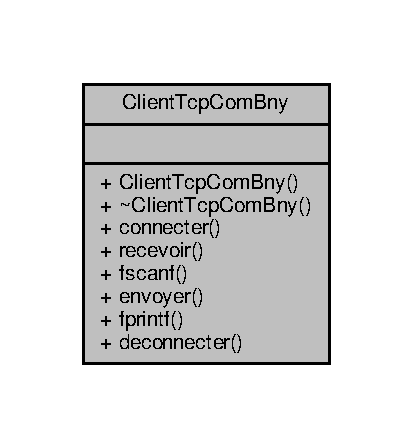
\includegraphics[width=198pt]{classClientTcpComBny__coll__graph}
\end{center}
\end{figure}
\subsection*{Fonctions membres publiques}
\begin{DoxyCompactItemize}
\item 
\hyperlink{classClientTcpComBny_a4e87071b400a5129f642a5a3721d420f}{Client\+Tcp\+Com\+Bny} ()
\item 
\hyperlink{classClientTcpComBny_ade30f75875dc873e2dc522228a7e5c68}{$\sim$\+Client\+Tcp\+Com\+Bny} ()
\item 
void \hyperlink{classClientTcpComBny_ac105b046c2e544b1a433f99d83d7447a}{connecter} (std\+::string ip, unsigned short int port)  throw (\+Tcp\+Ip\+Com\+Bny\+Exception)
\item 
void \hyperlink{classClientTcpComBny_ad32e6a288aeff3d243d88c60afe967c3}{recevoir} (char $\ast$buffer, std\+::size\+\_\+t size, std\+::size\+\_\+t \&count)  throw (\+Tcp\+Ip\+Com\+Bny\+Exception)
\item 
void \hyperlink{classClientTcpComBny_a0745845f86951740b6839812410608e8}{fscanf} (const char $\ast$format,...)
\item 
void \hyperlink{classClientTcpComBny_acf5ac7ad2c6815e6797a95f50906172f}{envoyer} (const char $\ast$buffer, std\+::size\+\_\+t size)  throw (\+Tcp\+Ip\+Com\+Bny\+Exception)
\item 
void \hyperlink{classClientTcpComBny_a3f2db7ecde5bf993a96bae8f4107e1c8}{fprintf} (const char $\ast$format,...)
\item 
void \hyperlink{classClientTcpComBny_aec1398f686da1f83884fd98924cc0725}{deconnecter} (void)
\end{DoxyCompactItemize}


\subsection{Documentation des constructeurs et destructeur}
\mbox{\Hypertarget{classClientTcpComBny_a4e87071b400a5129f642a5a3721d420f}\label{classClientTcpComBny_a4e87071b400a5129f642a5a3721d420f}} 
\index{Client\+Tcp\+Com\+Bny@{Client\+Tcp\+Com\+Bny}!Client\+Tcp\+Com\+Bny@{Client\+Tcp\+Com\+Bny}}
\index{Client\+Tcp\+Com\+Bny@{Client\+Tcp\+Com\+Bny}!Client\+Tcp\+Com\+Bny@{Client\+Tcp\+Com\+Bny}}
\subsubsection{\texorpdfstring{Client\+Tcp\+Com\+Bny()}{ClientTcpComBny()}}
{\footnotesize\ttfamily Client\+Tcp\+Com\+Bny\+::\+Client\+Tcp\+Com\+Bny (\begin{DoxyParamCaption}{ }\end{DoxyParamCaption})}

\mbox{\Hypertarget{classClientTcpComBny_ade30f75875dc873e2dc522228a7e5c68}\label{classClientTcpComBny_ade30f75875dc873e2dc522228a7e5c68}} 
\index{Client\+Tcp\+Com\+Bny@{Client\+Tcp\+Com\+Bny}!````~Client\+Tcp\+Com\+Bny@{$\sim$\+Client\+Tcp\+Com\+Bny}}
\index{````~Client\+Tcp\+Com\+Bny@{$\sim$\+Client\+Tcp\+Com\+Bny}!Client\+Tcp\+Com\+Bny@{Client\+Tcp\+Com\+Bny}}
\subsubsection{\texorpdfstring{$\sim$\+Client\+Tcp\+Com\+Bny()}{~ClientTcpComBny()}}
{\footnotesize\ttfamily Client\+Tcp\+Com\+Bny\+::$\sim$\+Client\+Tcp\+Com\+Bny (\begin{DoxyParamCaption}{ }\end{DoxyParamCaption})}



Références deconnecter().



\subsection{Documentation des fonctions membres}
\mbox{\Hypertarget{classClientTcpComBny_ac105b046c2e544b1a433f99d83d7447a}\label{classClientTcpComBny_ac105b046c2e544b1a433f99d83d7447a}} 
\index{Client\+Tcp\+Com\+Bny@{Client\+Tcp\+Com\+Bny}!connecter@{connecter}}
\index{connecter@{connecter}!Client\+Tcp\+Com\+Bny@{Client\+Tcp\+Com\+Bny}}
\subsubsection{\texorpdfstring{connecter()}{connecter()}}
{\footnotesize\ttfamily void Client\+Tcp\+Com\+Bny\+::connecter (\begin{DoxyParamCaption}\item[{std\+::string}]{ip,  }\item[{unsigned short int}]{port }\end{DoxyParamCaption}) throw  \hyperlink{classTcpIpComBnyException}{Tcp\+Ip\+Com\+Bny\+Exception}) }



Références Tcp\+Com\+Bny\+::fermer().

\mbox{\Hypertarget{classClientTcpComBny_aec1398f686da1f83884fd98924cc0725}\label{classClientTcpComBny_aec1398f686da1f83884fd98924cc0725}} 
\index{Client\+Tcp\+Com\+Bny@{Client\+Tcp\+Com\+Bny}!deconnecter@{deconnecter}}
\index{deconnecter@{deconnecter}!Client\+Tcp\+Com\+Bny@{Client\+Tcp\+Com\+Bny}}
\subsubsection{\texorpdfstring{deconnecter()}{deconnecter()}}
{\footnotesize\ttfamily void Client\+Tcp\+Com\+Bny\+::deconnecter (\begin{DoxyParamCaption}\item[{void}]{ }\end{DoxyParamCaption})}

\mbox{\Hypertarget{classClientTcpComBny_acf5ac7ad2c6815e6797a95f50906172f}\label{classClientTcpComBny_acf5ac7ad2c6815e6797a95f50906172f}} 
\index{Client\+Tcp\+Com\+Bny@{Client\+Tcp\+Com\+Bny}!envoyer@{envoyer}}
\index{envoyer@{envoyer}!Client\+Tcp\+Com\+Bny@{Client\+Tcp\+Com\+Bny}}
\subsubsection{\texorpdfstring{envoyer()}{envoyer()}}
{\footnotesize\ttfamily void Client\+Tcp\+Com\+Bny\+::envoyer (\begin{DoxyParamCaption}\item[{const char $\ast$}]{buffer,  }\item[{std\+::size\+\_\+t}]{size }\end{DoxyParamCaption}) throw  \hyperlink{classTcpIpComBnyException}{Tcp\+Ip\+Com\+Bny\+Exception}) }



Références Tcp\+Com\+Bny\+::envoyer().

\mbox{\Hypertarget{classClientTcpComBny_a3f2db7ecde5bf993a96bae8f4107e1c8}\label{classClientTcpComBny_a3f2db7ecde5bf993a96bae8f4107e1c8}} 
\index{Client\+Tcp\+Com\+Bny@{Client\+Tcp\+Com\+Bny}!fprintf@{fprintf}}
\index{fprintf@{fprintf}!Client\+Tcp\+Com\+Bny@{Client\+Tcp\+Com\+Bny}}
\subsubsection{\texorpdfstring{fprintf()}{fprintf()}}
{\footnotesize\ttfamily void Client\+Tcp\+Com\+Bny\+::fprintf (\begin{DoxyParamCaption}\item[{const char $\ast$}]{format,  }\item[{}]{... }\end{DoxyParamCaption})}



Références Tcp\+Com\+Bny\+::fprintf().

\mbox{\Hypertarget{classClientTcpComBny_a0745845f86951740b6839812410608e8}\label{classClientTcpComBny_a0745845f86951740b6839812410608e8}} 
\index{Client\+Tcp\+Com\+Bny@{Client\+Tcp\+Com\+Bny}!fscanf@{fscanf}}
\index{fscanf@{fscanf}!Client\+Tcp\+Com\+Bny@{Client\+Tcp\+Com\+Bny}}
\subsubsection{\texorpdfstring{fscanf()}{fscanf()}}
{\footnotesize\ttfamily void Client\+Tcp\+Com\+Bny\+::fscanf (\begin{DoxyParamCaption}\item[{const char $\ast$}]{format,  }\item[{}]{... }\end{DoxyParamCaption})}



Références Tcp\+Com\+Bny\+::fscanf().

\mbox{\Hypertarget{classClientTcpComBny_ad32e6a288aeff3d243d88c60afe967c3}\label{classClientTcpComBny_ad32e6a288aeff3d243d88c60afe967c3}} 
\index{Client\+Tcp\+Com\+Bny@{Client\+Tcp\+Com\+Bny}!recevoir@{recevoir}}
\index{recevoir@{recevoir}!Client\+Tcp\+Com\+Bny@{Client\+Tcp\+Com\+Bny}}
\subsubsection{\texorpdfstring{recevoir()}{recevoir()}}
{\footnotesize\ttfamily void Client\+Tcp\+Com\+Bny\+::recevoir (\begin{DoxyParamCaption}\item[{char $\ast$}]{buffer,  }\item[{std\+::size\+\_\+t}]{size,  }\item[{std\+::size\+\_\+t \&}]{count }\end{DoxyParamCaption}) throw  \hyperlink{classTcpIpComBnyException}{Tcp\+Ip\+Com\+Bny\+Exception}) }



Références Tcp\+Com\+Bny\+::recevoir().



La documentation de cette classe a été générée à partir des fichiers suivants \+:\begin{DoxyCompactItemize}
\item 
src/\hyperlink{ClientTcpComBny_8h}{Client\+Tcp\+Com\+Bny.\+h}\item 
src/\hyperlink{ClientTcpComBny_8cpp}{Client\+Tcp\+Com\+Bny.\+cpp}\end{DoxyCompactItemize}

\hypertarget{classEclairage_1_1Controleur}{}\section{Référence de la classe Eclairage\+:\+:Controleur}
\label{classEclairage_1_1Controleur}\index{Eclairage\+::\+Controleur@{Eclairage\+::\+Controleur}}


{\ttfamily \#include $<$Eclairage.\+h$>$}



Graphe d\textquotesingle{}héritage de Eclairage\+:\+:Controleur\+:\nopagebreak
\begin{figure}[H]
\begin{center}
\leavevmode
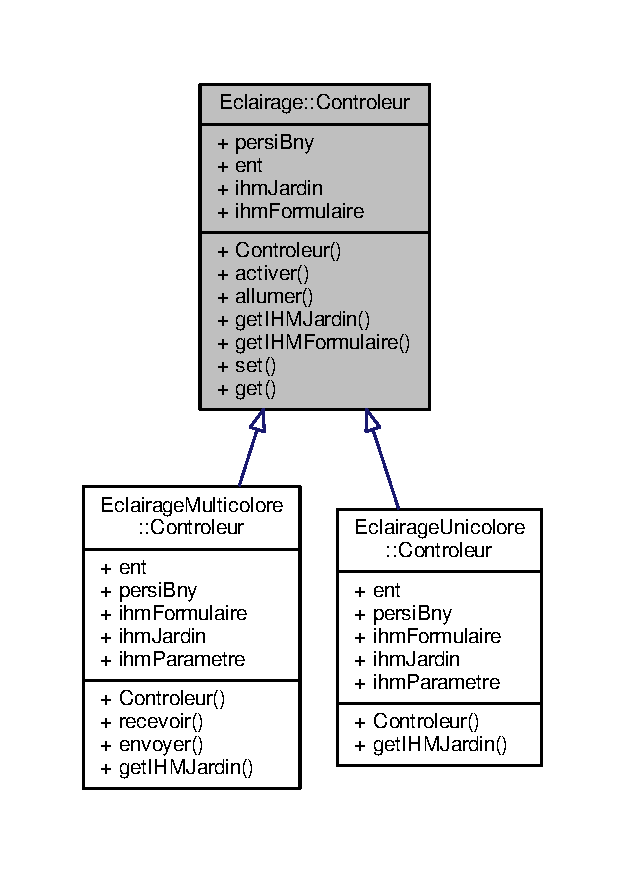
\includegraphics[width=300pt]{classEclairage_1_1Controleur__inherit__graph}
\end{center}
\end{figure}


Graphe de collaboration de Eclairage\+:\+:Controleur\+:\nopagebreak
\begin{figure}[H]
\begin{center}
\leavevmode
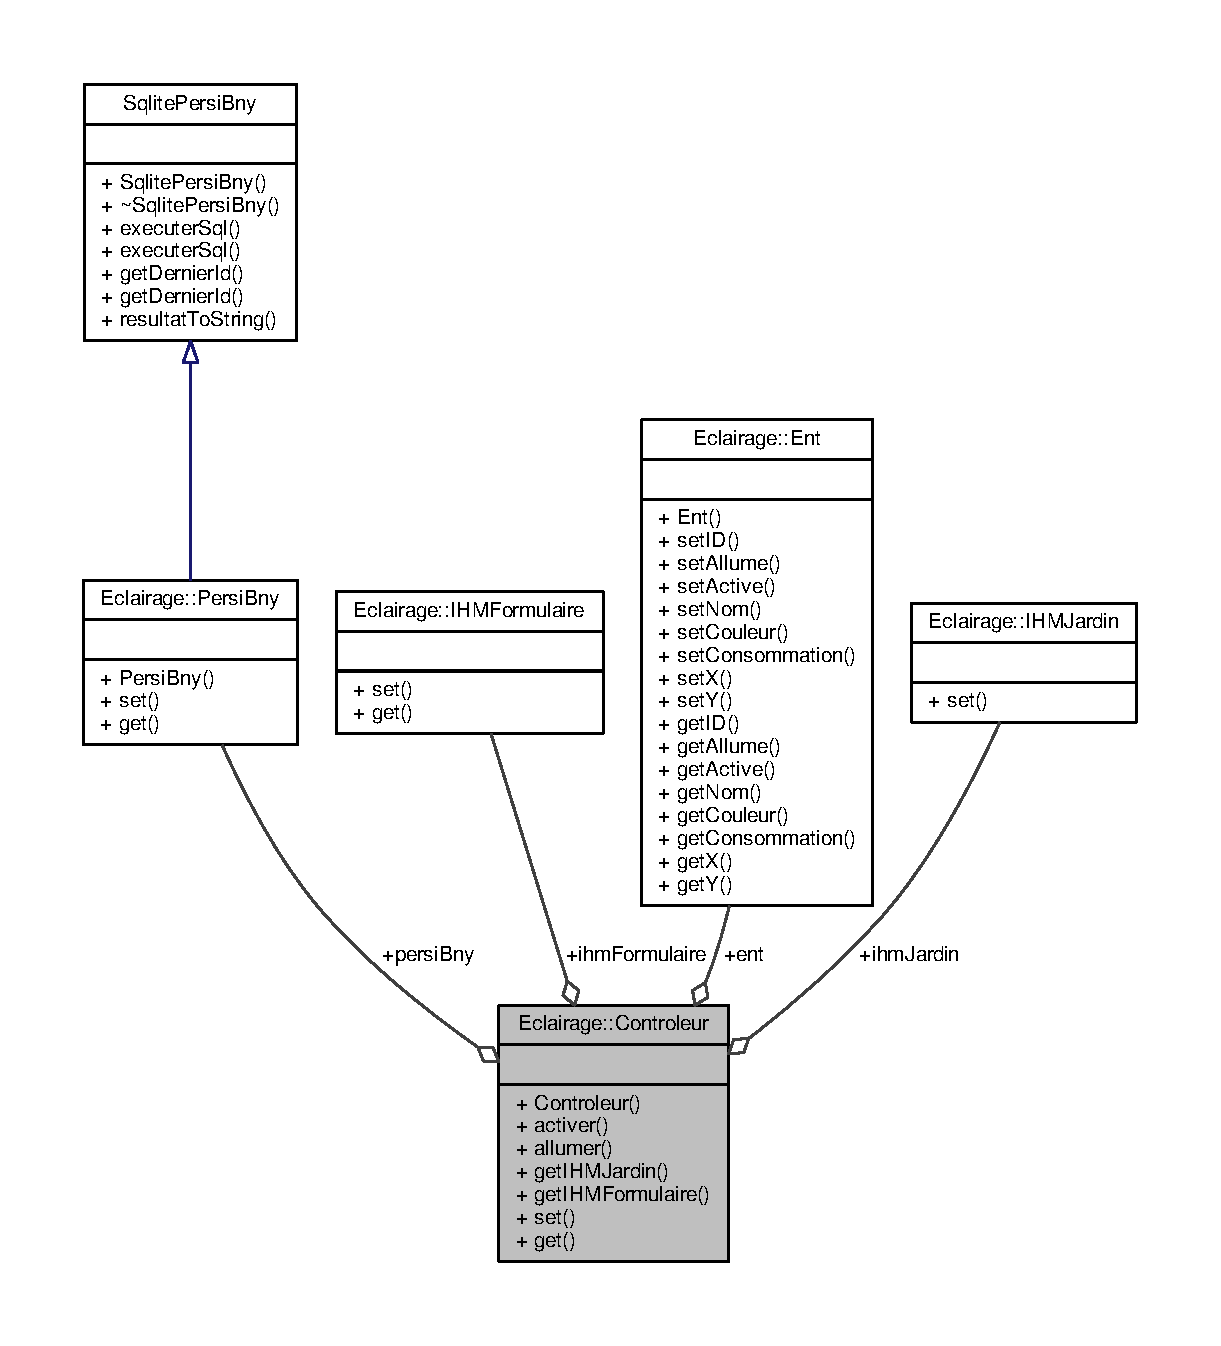
\includegraphics[width=190pt]{classEclairage_1_1Controleur__coll__graph}
\end{center}
\end{figure}
\subsection*{Fonctions membres publiques}
\begin{DoxyCompactItemize}
\item 
void \hyperlink{classEclairage_1_1Controleur_abdf832d1dba32ae0cae84009022704ae}{activer} (bool etat)
\item 
void \hyperlink{classEclairage_1_1Controleur_acca8b13291f05a3e65a0c628409d65f4}{allumer} (bool etat)
\item 
void \hyperlink{classEclairage_1_1Controleur_a4962daee48ffa6cd40d01623a4506d04}{get\+I\+H\+M\+Jardin} ()
\item 
void \hyperlink{classEclairage_1_1Controleur_a3fa6d8e23e50c00383913259a8a14162}{get\+I\+H\+M\+Formulaire} ()
\item 
void \hyperlink{classEclairage_1_1Controleur_a5a9e725e98db67bd3a584a3819b269f6}{set} (const \hyperlink{classEclairage_1_1Ent}{Ent} \&ent)
\item 
void \hyperlink{classEclairage_1_1Controleur_aaa82a14322c2a354aacb0787a6532105}{get} (\hyperlink{classEclairage_1_1Ent}{Ent} \&ent)
\end{DoxyCompactItemize}


\subsection{Description détaillée}
\hyperlink{classEclairage_1_1Controleur}{Controleur} de la classe eclairage. 

\subsection{Documentation des fonctions membres}
\mbox{\Hypertarget{classEclairage_1_1Controleur_abdf832d1dba32ae0cae84009022704ae}\label{classEclairage_1_1Controleur_abdf832d1dba32ae0cae84009022704ae}} 
\index{Eclairage\+::\+Controleur@{Eclairage\+::\+Controleur}!activer@{activer}}
\index{activer@{activer}!Eclairage\+::\+Controleur@{Eclairage\+::\+Controleur}}
\subsubsection{\texorpdfstring{activer()}{activer()}}
{\footnotesize\ttfamily void Eclairage\+::\+Controleur\+::activer (\begin{DoxyParamCaption}\item[{bool}]{etat }\end{DoxyParamCaption})}

M�thode permettant d\textquotesingle{}activer/d�sactiver l\textquotesingle{}�clairage en fonction d\textquotesingle{}un bool�en pass� en param�tres. \mbox{\Hypertarget{classEclairage_1_1Controleur_acca8b13291f05a3e65a0c628409d65f4}\label{classEclairage_1_1Controleur_acca8b13291f05a3e65a0c628409d65f4}} 
\index{Eclairage\+::\+Controleur@{Eclairage\+::\+Controleur}!allumer@{allumer}}
\index{allumer@{allumer}!Eclairage\+::\+Controleur@{Eclairage\+::\+Controleur}}
\subsubsection{\texorpdfstring{allumer()}{allumer()}}
{\footnotesize\ttfamily void Eclairage\+::\+Controleur\+::allumer (\begin{DoxyParamCaption}\item[{bool}]{etat }\end{DoxyParamCaption})}

M�thode permettant d\textquotesingle{}allumer/�teindre un �clairage gr�ce � un bool�en pass� en param�tre. \mbox{\Hypertarget{classEclairage_1_1Controleur_aaa82a14322c2a354aacb0787a6532105}\label{classEclairage_1_1Controleur_aaa82a14322c2a354aacb0787a6532105}} 
\index{Eclairage\+::\+Controleur@{Eclairage\+::\+Controleur}!get@{get}}
\index{get@{get}!Eclairage\+::\+Controleur@{Eclairage\+::\+Controleur}}
\subsubsection{\texorpdfstring{get()}{get()}}
{\footnotesize\ttfamily void Eclairage\+::\+Controleur\+::get (\begin{DoxyParamCaption}\item[{\hyperlink{classEclairage_1_1Ent}{Eclairage\+::\+Ent} \&}]{ent }\end{DoxyParamCaption})}

M�thode permettant de r�cup�rer l\textquotesingle{}entit� de l\textquotesingle{}�clairage. \mbox{\Hypertarget{classEclairage_1_1Controleur_a3fa6d8e23e50c00383913259a8a14162}\label{classEclairage_1_1Controleur_a3fa6d8e23e50c00383913259a8a14162}} 
\index{Eclairage\+::\+Controleur@{Eclairage\+::\+Controleur}!get\+I\+H\+M\+Formulaire@{get\+I\+H\+M\+Formulaire}}
\index{get\+I\+H\+M\+Formulaire@{get\+I\+H\+M\+Formulaire}!Eclairage\+::\+Controleur@{Eclairage\+::\+Controleur}}
\subsubsection{\texorpdfstring{get\+I\+H\+M\+Formulaire()}{getIHMFormulaire()}}
{\footnotesize\ttfamily void Eclairage\+::\+Controleur\+::get\+I\+H\+M\+Formulaire (\begin{DoxyParamCaption}{ }\end{DoxyParamCaption})}

M�thode permettant de r�cup�rer les informations entr�es par le propri�taire lors de la cr�ation de l\textquotesingle{}�clairage. \mbox{\Hypertarget{classEclairage_1_1Controleur_a4962daee48ffa6cd40d01623a4506d04}\label{classEclairage_1_1Controleur_a4962daee48ffa6cd40d01623a4506d04}} 
\index{Eclairage\+::\+Controleur@{Eclairage\+::\+Controleur}!get\+I\+H\+M\+Jardin@{get\+I\+H\+M\+Jardin}}
\index{get\+I\+H\+M\+Jardin@{get\+I\+H\+M\+Jardin}!Eclairage\+::\+Controleur@{Eclairage\+::\+Controleur}}
\subsubsection{\texorpdfstring{get\+I\+H\+M\+Jardin()}{getIHMJardin()}}
{\footnotesize\ttfamily void Eclairage\+::\+Controleur\+::get\+I\+H\+M\+Jardin (\begin{DoxyParamCaption}{ }\end{DoxyParamCaption})}

M�thode permettant de r�cup�rer l\textquotesingle{}�tat de l\textquotesingle{}\hyperlink{classEclairage_1_1IHMJardin}{I\+H\+M\+Jardin} (Icone repr�sentant l\textquotesingle{}�clairage dans l\textquotesingle{}I\+HM de supervision) \mbox{\Hypertarget{classEclairage_1_1Controleur_a5a9e725e98db67bd3a584a3819b269f6}\label{classEclairage_1_1Controleur_a5a9e725e98db67bd3a584a3819b269f6}} 
\index{Eclairage\+::\+Controleur@{Eclairage\+::\+Controleur}!set@{set}}
\index{set@{set}!Eclairage\+::\+Controleur@{Eclairage\+::\+Controleur}}
\subsubsection{\texorpdfstring{set()}{set()}}
{\footnotesize\ttfamily void Eclairage\+::\+Controleur\+::set (\begin{DoxyParamCaption}\item[{const \hyperlink{classEclairage_1_1Ent}{Ent} \&}]{ent }\end{DoxyParamCaption})}

M�thode permettant de modifier int�gralement la configuration de l\textquotesingle{}�clairage en lui passant une entit� en param�tres. 

La documentation de cette classe a été générée à partir des fichiers suivants \+:\begin{DoxyCompactItemize}
\item 
src/\hyperlink{Eclairage_8h}{Eclairage.\+h}\item 
src/\hyperlink{Eclairage_8cpp}{Eclairage.\+cpp}\end{DoxyCompactItemize}

\hypertarget{classEclairageMulticolore_1_1Controleur}{}\section{Référence de la classe Eclairage\+Multicolore\+:\+:Controleur}
\label{classEclairageMulticolore_1_1Controleur}\index{Eclairage\+Multicolore\+::\+Controleur@{Eclairage\+Multicolore\+::\+Controleur}}


{\ttfamily \#include $<$Eclairage\+Multicolore.\+h$>$}



Graphe d\textquotesingle{}héritage de Eclairage\+Multicolore\+:\+:Controleur\+:\nopagebreak
\begin{figure}[H]
\begin{center}
\leavevmode
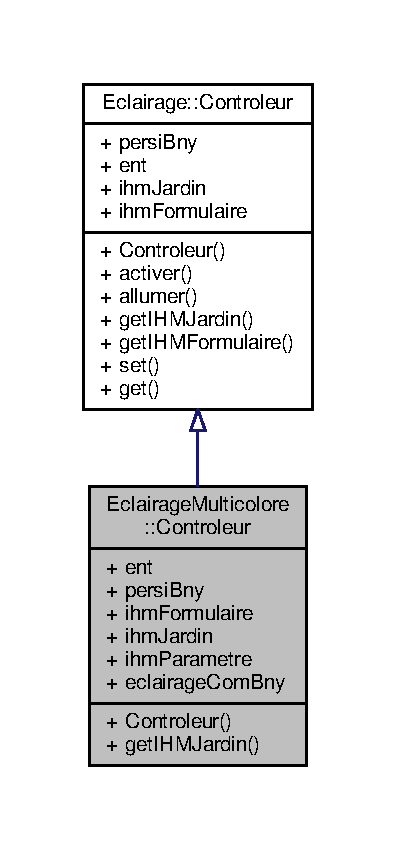
\includegraphics[width=190pt]{classEclairageMulticolore_1_1Controleur__inherit__graph}
\end{center}
\end{figure}


Graphe de collaboration de Eclairage\+Multicolore\+:\+:Controleur\+:\nopagebreak
\begin{figure}[H]
\begin{center}
\leavevmode
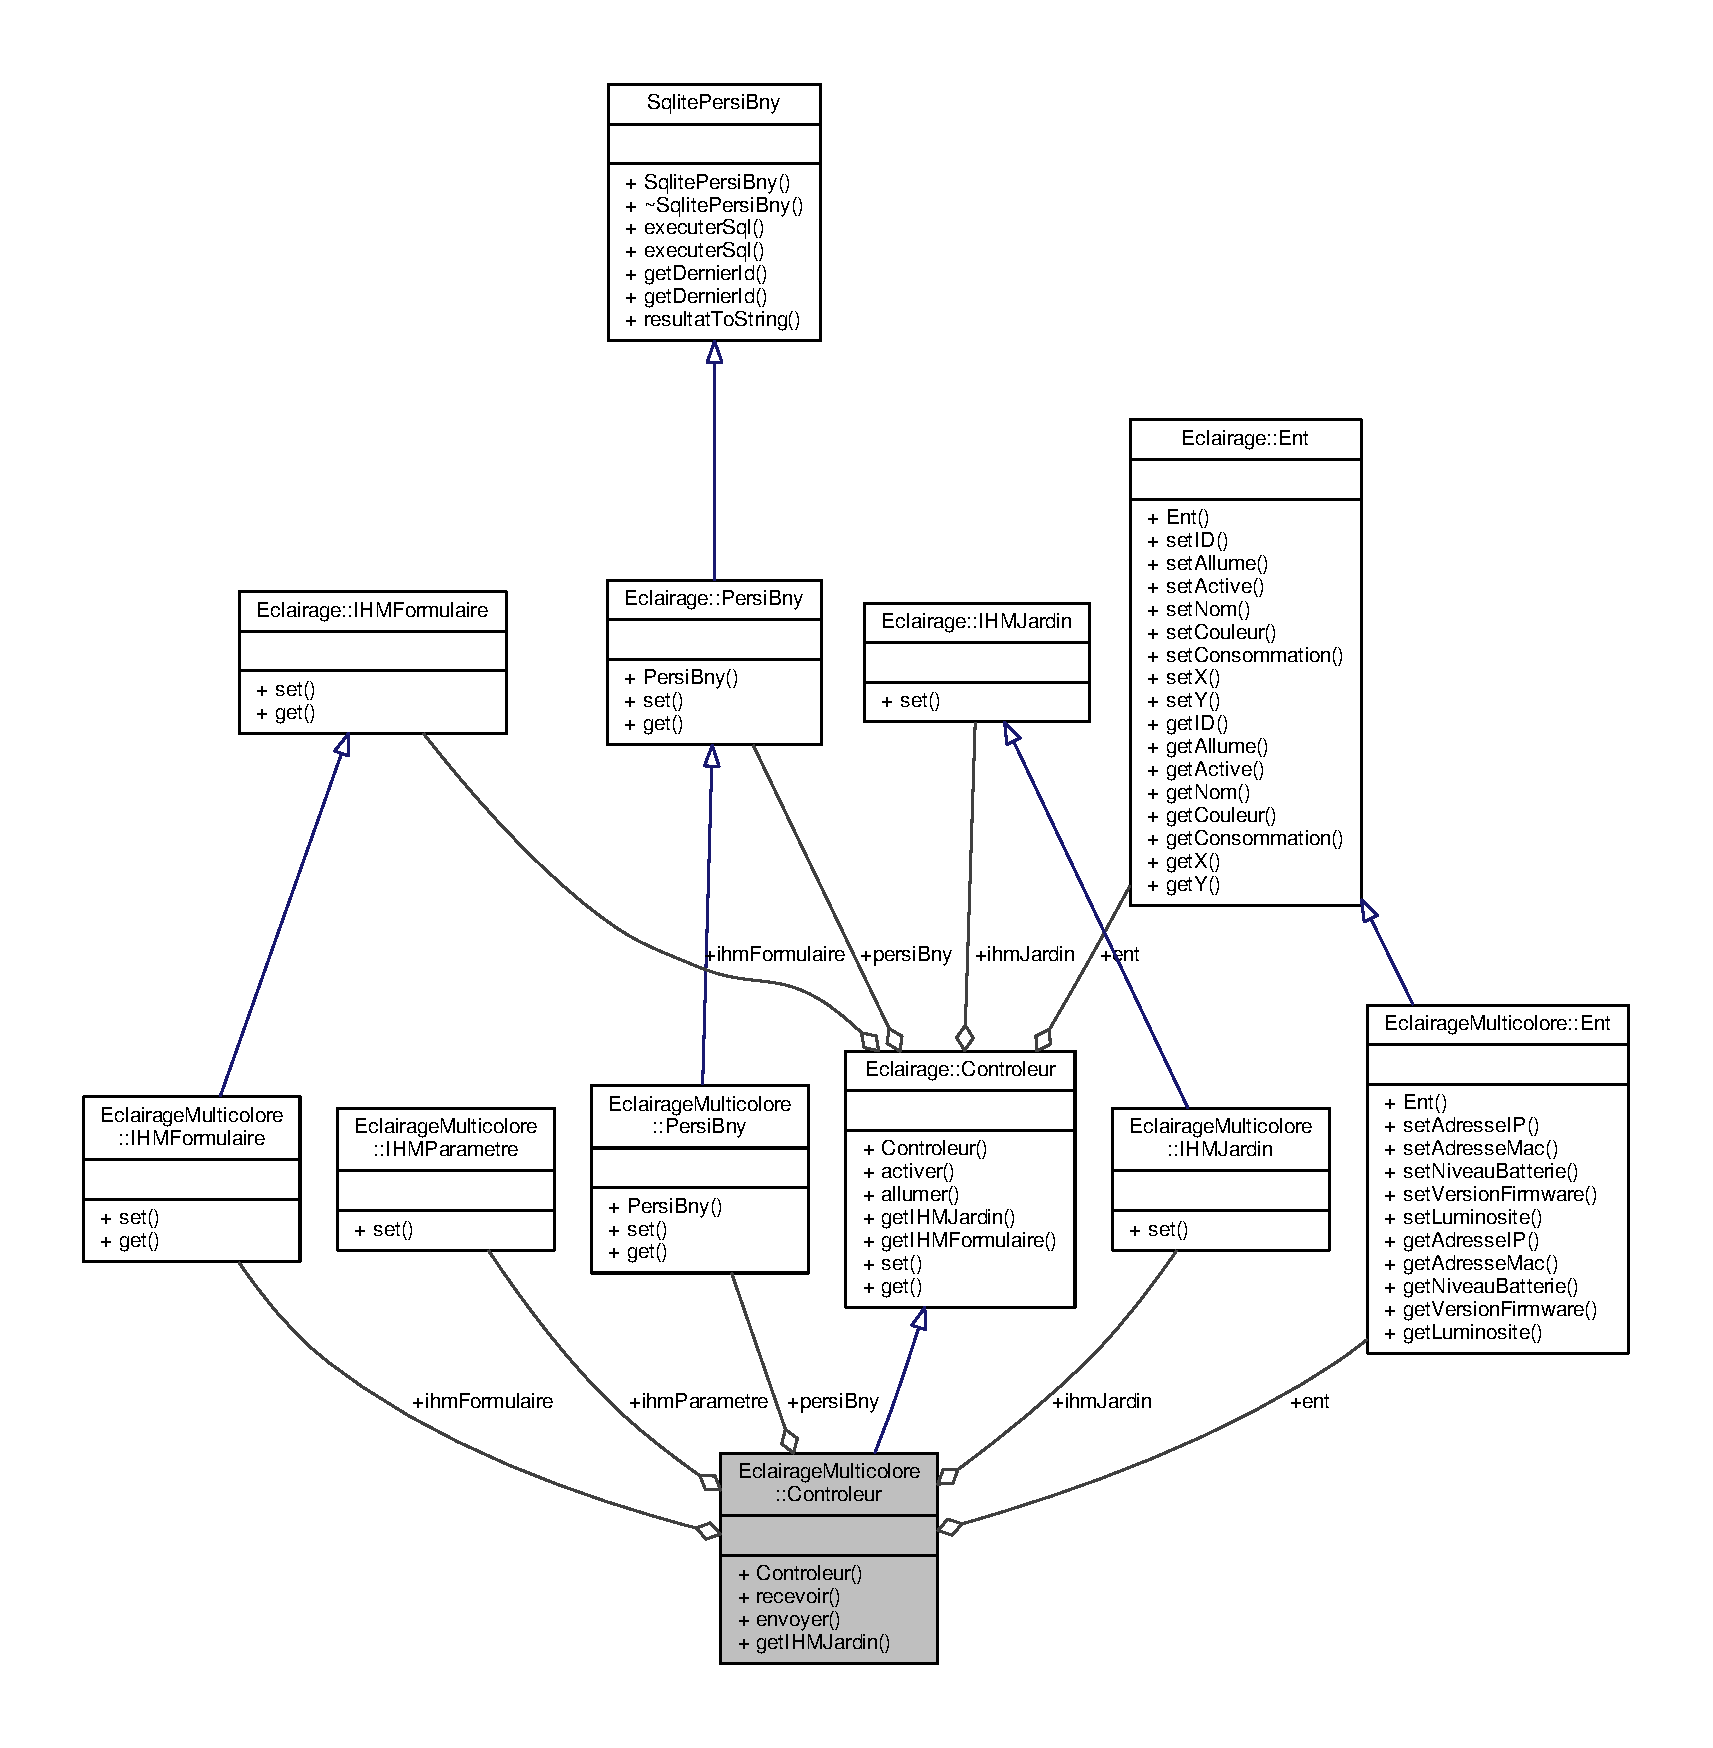
\includegraphics[width=190pt]{classEclairageMulticolore_1_1Controleur__coll__graph}
\end{center}
\end{figure}
\subsection*{Fonctions membres publiques}
\begin{DoxyCompactItemize}
\item 
void \hyperlink{classEclairageMulticolore_1_1Controleur_af9c385233534bf62ede4f97b9e823105}{recevoir} ()
\item 
void \hyperlink{classEclairageMulticolore_1_1Controleur_ac73fb221d85530dd039312caf6720e99}{envoyer} ()
\end{DoxyCompactItemize}


\subsection{Documentation des fonctions membres}
\mbox{\Hypertarget{classEclairageMulticolore_1_1Controleur_ac73fb221d85530dd039312caf6720e99}\label{classEclairageMulticolore_1_1Controleur_ac73fb221d85530dd039312caf6720e99}} 
\index{Eclairage\+Multicolore\+::\+Controleur@{Eclairage\+Multicolore\+::\+Controleur}!envoyer@{envoyer}}
\index{envoyer@{envoyer}!Eclairage\+Multicolore\+::\+Controleur@{Eclairage\+Multicolore\+::\+Controleur}}
\subsubsection{\texorpdfstring{envoyer()}{envoyer()}}
{\footnotesize\ttfamily void Eclairage\+Multicolore\+::\+Controleur\+::envoyer (\begin{DoxyParamCaption}{ }\end{DoxyParamCaption})}

M�thode permettant d\textquotesingle{}envoyer une configuration d\textquotesingle{}eclairage via le r�seau. \mbox{\Hypertarget{classEclairageMulticolore_1_1Controleur_af9c385233534bf62ede4f97b9e823105}\label{classEclairageMulticolore_1_1Controleur_af9c385233534bf62ede4f97b9e823105}} 
\index{Eclairage\+Multicolore\+::\+Controleur@{Eclairage\+Multicolore\+::\+Controleur}!recevoir@{recevoir}}
\index{recevoir@{recevoir}!Eclairage\+Multicolore\+::\+Controleur@{Eclairage\+Multicolore\+::\+Controleur}}
\subsubsection{\texorpdfstring{recevoir()}{recevoir()}}
{\footnotesize\ttfamily void Eclairage\+Multicolore\+::\+Controleur\+::recevoir (\begin{DoxyParamCaption}{ }\end{DoxyParamCaption})}

M�thode permettant de recevoir une configuration d\textquotesingle{}�clairage via le r�seau. 

La documentation de cette classe a été générée à partir des fichiers suivants \+:\begin{DoxyCompactItemize}
\item 
src/\hyperlink{EclairageMulticolore_8h}{Eclairage\+Multicolore.\+h}\item 
src/\hyperlink{EclairageMulticolore_8cpp}{Eclairage\+Multicolore.\+cpp}\end{DoxyCompactItemize}

\hypertarget{classEclairageUnicolore_1_1Controleur}{}\section{Référence de la classe Eclairage\+Unicolore\+:\+:Controleur}
\label{classEclairageUnicolore_1_1Controleur}\index{Eclairage\+Unicolore\+::\+Controleur@{Eclairage\+Unicolore\+::\+Controleur}}


{\ttfamily \#include $<$Eclairage\+Unicolore.\+h$>$}



Graphe d\textquotesingle{}héritage de Eclairage\+Unicolore\+:\+:Controleur\+:
\nopagebreak
\begin{figure}[H]
\begin{center}
\leavevmode
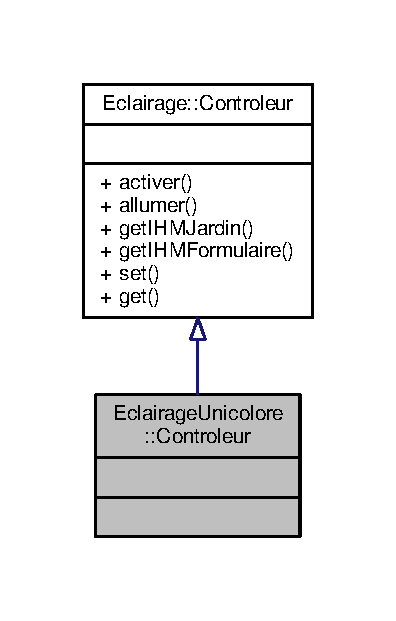
\includegraphics[width=190pt]{classEclairageUnicolore_1_1Controleur__inherit__graph}
\end{center}
\end{figure}


Graphe de collaboration de Eclairage\+Unicolore\+:\+:Controleur\+:
\nopagebreak
\begin{figure}[H]
\begin{center}
\leavevmode
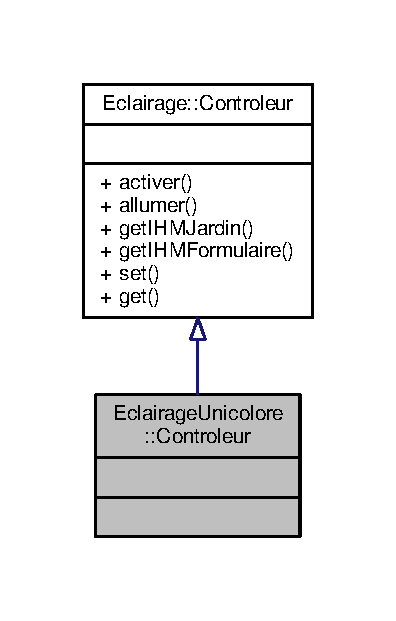
\includegraphics[width=350pt]{classEclairageUnicolore_1_1Controleur__coll__graph}
\end{center}
\end{figure}
\subsection*{Fonctions membres publiques}
\begin{DoxyCompactItemize}
\item 
\hyperlink{classEclairageUnicolore_1_1Controleur_aa4c04918511034c561f5e31872a5d6fb}{Controleur} ()
\item 
void \hyperlink{classEclairageUnicolore_1_1Controleur_a911f1e20ccdac1faf9dbf2fe42e209fb}{get\+I\+H\+M\+Jardin} ()
\end{DoxyCompactItemize}
\subsection*{Attributs publics}
\begin{DoxyCompactItemize}
\item 
\hyperlink{classEclairageUnicolore_1_1Ent}{Ent} \hyperlink{classEclairageUnicolore_1_1Controleur_a7405ea9580f0a795d73fe9d28e7d52d2}{ent}
\item 
\hyperlink{classEclairageUnicolore_1_1PersiBny}{Persi\+Bny} \hyperlink{classEclairageUnicolore_1_1Controleur_a75cc9ad70e00f85567ea9e35bdd0299b}{persi\+Bny}
\item 
\hyperlink{classEclairageUnicolore_1_1IHMFormulaire}{I\+H\+M\+Formulaire} \hyperlink{classEclairageUnicolore_1_1Controleur_a4beb9ae5d84acb0fa92217e7a2c12903}{ihm\+Formulaire}
\item 
\hyperlink{classEclairageUnicolore_1_1IHMJardin}{I\+H\+M\+Jardin} \hyperlink{classEclairageUnicolore_1_1Controleur_a5ff7285164d9b88024f3da2e7aa32032}{ihm\+Jardin}
\item 
\hyperlink{classEclairageUnicolore_1_1IHMParametre}{I\+H\+M\+Parametre} \hyperlink{classEclairageUnicolore_1_1Controleur_a5b4225363002c9f4cda34e9d2252fb3b}{ihm\+Parametre}
\item 
\hyperlink{classEclairageUnicolore_1_1EclairageComBny}{Eclairage\+Com\+Bny} \hyperlink{classEclairageUnicolore_1_1Controleur_aaff6697834f75bb05777f6339e153061}{eclairage\+Com\+Bny}
\end{DoxyCompactItemize}


\subsection{Description détaillée}
Classe controleur contenant une entit�, une persistance et une \hyperlink{classEclairageUnicolore_1_1IHMFormulaire}{I\+H\+M\+Formulaire} de cr�ation. 

\subsection{Documentation des constructeurs et destructeur}
\mbox{\Hypertarget{classEclairageUnicolore_1_1Controleur_aa4c04918511034c561f5e31872a5d6fb}\label{classEclairageUnicolore_1_1Controleur_aa4c04918511034c561f5e31872a5d6fb}} 
\index{Eclairage\+Unicolore\+::\+Controleur@{Eclairage\+Unicolore\+::\+Controleur}!Controleur@{Controleur}}
\index{Controleur@{Controleur}!Eclairage\+Unicolore\+::\+Controleur@{Eclairage\+Unicolore\+::\+Controleur}}
\subsubsection{\texorpdfstring{Controleur()}{Controleur()}}
{\footnotesize\ttfamily Eclairage\+Unicolore\+::\+Controleur\+::\+Controleur (\begin{DoxyParamCaption}{ }\end{DoxyParamCaption})\hspace{0.3cm}{\ttfamily [inline]}}



\subsection{Documentation des fonctions membres}
\mbox{\Hypertarget{classEclairageUnicolore_1_1Controleur_a911f1e20ccdac1faf9dbf2fe42e209fb}\label{classEclairageUnicolore_1_1Controleur_a911f1e20ccdac1faf9dbf2fe42e209fb}} 
\index{Eclairage\+Unicolore\+::\+Controleur@{Eclairage\+Unicolore\+::\+Controleur}!get\+I\+H\+M\+Jardin@{get\+I\+H\+M\+Jardin}}
\index{get\+I\+H\+M\+Jardin@{get\+I\+H\+M\+Jardin}!Eclairage\+Unicolore\+::\+Controleur@{Eclairage\+Unicolore\+::\+Controleur}}
\subsubsection{\texorpdfstring{get\+I\+H\+M\+Jardin()}{getIHMJardin()}}
{\footnotesize\ttfamily void Eclairage\+Unicolore\+::\+Controleur\+::get\+I\+H\+M\+Jardin (\begin{DoxyParamCaption}{ }\end{DoxyParamCaption})}



\subsection{Documentation des données membres}
\mbox{\Hypertarget{classEclairageUnicolore_1_1Controleur_aaff6697834f75bb05777f6339e153061}\label{classEclairageUnicolore_1_1Controleur_aaff6697834f75bb05777f6339e153061}} 
\index{Eclairage\+Unicolore\+::\+Controleur@{Eclairage\+Unicolore\+::\+Controleur}!eclairage\+Com\+Bny@{eclairage\+Com\+Bny}}
\index{eclairage\+Com\+Bny@{eclairage\+Com\+Bny}!Eclairage\+Unicolore\+::\+Controleur@{Eclairage\+Unicolore\+::\+Controleur}}
\subsubsection{\texorpdfstring{eclairage\+Com\+Bny}{eclairageComBny}}
{\footnotesize\ttfamily \hyperlink{classEclairageUnicolore_1_1EclairageComBny}{Eclairage\+Com\+Bny} Eclairage\+Unicolore\+::\+Controleur\+::eclairage\+Com\+Bny}

\mbox{\Hypertarget{classEclairageUnicolore_1_1Controleur_a7405ea9580f0a795d73fe9d28e7d52d2}\label{classEclairageUnicolore_1_1Controleur_a7405ea9580f0a795d73fe9d28e7d52d2}} 
\index{Eclairage\+Unicolore\+::\+Controleur@{Eclairage\+Unicolore\+::\+Controleur}!ent@{ent}}
\index{ent@{ent}!Eclairage\+Unicolore\+::\+Controleur@{Eclairage\+Unicolore\+::\+Controleur}}
\subsubsection{\texorpdfstring{ent}{ent}}
{\footnotesize\ttfamily \hyperlink{classEclairageUnicolore_1_1Ent}{Ent} Eclairage\+Unicolore\+::\+Controleur\+::ent}

\mbox{\Hypertarget{classEclairageUnicolore_1_1Controleur_a4beb9ae5d84acb0fa92217e7a2c12903}\label{classEclairageUnicolore_1_1Controleur_a4beb9ae5d84acb0fa92217e7a2c12903}} 
\index{Eclairage\+Unicolore\+::\+Controleur@{Eclairage\+Unicolore\+::\+Controleur}!ihm\+Formulaire@{ihm\+Formulaire}}
\index{ihm\+Formulaire@{ihm\+Formulaire}!Eclairage\+Unicolore\+::\+Controleur@{Eclairage\+Unicolore\+::\+Controleur}}
\subsubsection{\texorpdfstring{ihm\+Formulaire}{ihmFormulaire}}
{\footnotesize\ttfamily \hyperlink{classEclairageUnicolore_1_1IHMFormulaire}{I\+H\+M\+Formulaire} Eclairage\+Unicolore\+::\+Controleur\+::ihm\+Formulaire}

\mbox{\Hypertarget{classEclairageUnicolore_1_1Controleur_a5ff7285164d9b88024f3da2e7aa32032}\label{classEclairageUnicolore_1_1Controleur_a5ff7285164d9b88024f3da2e7aa32032}} 
\index{Eclairage\+Unicolore\+::\+Controleur@{Eclairage\+Unicolore\+::\+Controleur}!ihm\+Jardin@{ihm\+Jardin}}
\index{ihm\+Jardin@{ihm\+Jardin}!Eclairage\+Unicolore\+::\+Controleur@{Eclairage\+Unicolore\+::\+Controleur}}
\subsubsection{\texorpdfstring{ihm\+Jardin}{ihmJardin}}
{\footnotesize\ttfamily \hyperlink{classEclairageUnicolore_1_1IHMJardin}{I\+H\+M\+Jardin} Eclairage\+Unicolore\+::\+Controleur\+::ihm\+Jardin}

\mbox{\Hypertarget{classEclairageUnicolore_1_1Controleur_a5b4225363002c9f4cda34e9d2252fb3b}\label{classEclairageUnicolore_1_1Controleur_a5b4225363002c9f4cda34e9d2252fb3b}} 
\index{Eclairage\+Unicolore\+::\+Controleur@{Eclairage\+Unicolore\+::\+Controleur}!ihm\+Parametre@{ihm\+Parametre}}
\index{ihm\+Parametre@{ihm\+Parametre}!Eclairage\+Unicolore\+::\+Controleur@{Eclairage\+Unicolore\+::\+Controleur}}
\subsubsection{\texorpdfstring{ihm\+Parametre}{ihmParametre}}
{\footnotesize\ttfamily \hyperlink{classEclairageUnicolore_1_1IHMParametre}{I\+H\+M\+Parametre} Eclairage\+Unicolore\+::\+Controleur\+::ihm\+Parametre}

\mbox{\Hypertarget{classEclairageUnicolore_1_1Controleur_a75cc9ad70e00f85567ea9e35bdd0299b}\label{classEclairageUnicolore_1_1Controleur_a75cc9ad70e00f85567ea9e35bdd0299b}} 
\index{Eclairage\+Unicolore\+::\+Controleur@{Eclairage\+Unicolore\+::\+Controleur}!persi\+Bny@{persi\+Bny}}
\index{persi\+Bny@{persi\+Bny}!Eclairage\+Unicolore\+::\+Controleur@{Eclairage\+Unicolore\+::\+Controleur}}
\subsubsection{\texorpdfstring{persi\+Bny}{persiBny}}
{\footnotesize\ttfamily \hyperlink{classEclairageUnicolore_1_1PersiBny}{Persi\+Bny} Eclairage\+Unicolore\+::\+Controleur\+::persi\+Bny}



La documentation de cette classe a été générée à partir des fichiers suivants \+:\begin{DoxyCompactItemize}
\item 
src/\hyperlink{EclairageUnicolore_8h}{Eclairage\+Unicolore.\+h}\item 
src/\hyperlink{EclairageUnicolore_8cpp}{Eclairage\+Unicolore.\+cpp}\end{DoxyCompactItemize}

\hypertarget{classCSV}{}\section{Référence de la classe C\+SV}
\label{classCSV}\index{C\+SV@{C\+SV}}


{\ttfamily \#include $<$csv.\+h$>$}



Graphe de collaboration de C\+SV\+:
\nopagebreak
\begin{figure}[H]
\begin{center}
\leavevmode
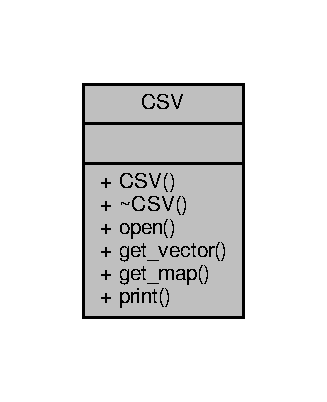
\includegraphics[width=157pt]{classCSV__coll__graph}
\end{center}
\end{figure}
\subsection*{Fonctions membres publiques}
\begin{DoxyCompactItemize}
\item 
\hyperlink{classCSV_a335bef6309d648d44907c0e7279cc32c}{C\+SV} ()
\item 
\hyperlink{classCSV_ae1b0cfd98d62cf81004462320848c665}{$\sim$\+C\+SV} ()
\item 
void \hyperlink{classCSV_a80fbeab0aad2b0695d0720cc863826b8}{open} (std\+::string filename)
\item 
std\+::vector$<$ std\+::vector$<$ std\+::string $>$ $>$ \hyperlink{classCSV_a62f788e022970a4e847a8850efa9d75a}{get\+\_\+vector} ()
\item 
std\+::map$<$ std\+::string, std\+::vector$<$ std\+::string $>$ $>$ \hyperlink{classCSV_af29150140f6e2ad4a75928fbb1ff23a7}{get\+\_\+map} (bool head=true)
\item 
void \hyperlink{classCSV_aabdbae3a626d0bc5a0dc573c9161f0a9}{print} ()
\end{DoxyCompactItemize}


\subsection{Documentation des constructeurs et destructeur}
\mbox{\Hypertarget{classCSV_a335bef6309d648d44907c0e7279cc32c}\label{classCSV_a335bef6309d648d44907c0e7279cc32c}} 
\index{C\+SV@{C\+SV}!C\+SV@{C\+SV}}
\index{C\+SV@{C\+SV}!C\+SV@{C\+SV}}
\subsubsection{\texorpdfstring{C\+S\+V()}{CSV()}}
{\footnotesize\ttfamily C\+S\+V\+::\+C\+SV (\begin{DoxyParamCaption}{ }\end{DoxyParamCaption})}

\mbox{\Hypertarget{classCSV_ae1b0cfd98d62cf81004462320848c665}\label{classCSV_ae1b0cfd98d62cf81004462320848c665}} 
\index{C\+SV@{C\+SV}!````~C\+SV@{$\sim$\+C\+SV}}
\index{````~C\+SV@{$\sim$\+C\+SV}!C\+SV@{C\+SV}}
\subsubsection{\texorpdfstring{$\sim$\+C\+S\+V()}{~CSV()}}
{\footnotesize\ttfamily C\+S\+V\+::$\sim$\+C\+SV (\begin{DoxyParamCaption}{ }\end{DoxyParamCaption})}



\subsection{Documentation des fonctions membres}
\mbox{\Hypertarget{classCSV_af29150140f6e2ad4a75928fbb1ff23a7}\label{classCSV_af29150140f6e2ad4a75928fbb1ff23a7}} 
\index{C\+SV@{C\+SV}!get\+\_\+map@{get\+\_\+map}}
\index{get\+\_\+map@{get\+\_\+map}!C\+SV@{C\+SV}}
\subsubsection{\texorpdfstring{get\+\_\+map()}{get\_map()}}
{\footnotesize\ttfamily map$<$ string, vector$<$ string $>$ $>$ C\+S\+V\+::get\+\_\+map (\begin{DoxyParamCaption}\item[{bool}]{head = {\ttfamily true} }\end{DoxyParamCaption})}

\mbox{\Hypertarget{classCSV_a62f788e022970a4e847a8850efa9d75a}\label{classCSV_a62f788e022970a4e847a8850efa9d75a}} 
\index{C\+SV@{C\+SV}!get\+\_\+vector@{get\+\_\+vector}}
\index{get\+\_\+vector@{get\+\_\+vector}!C\+SV@{C\+SV}}
\subsubsection{\texorpdfstring{get\+\_\+vector()}{get\_vector()}}
{\footnotesize\ttfamily vector$<$ std\+::vector$<$ std\+::string $>$ $>$ C\+S\+V\+::get\+\_\+vector (\begin{DoxyParamCaption}{ }\end{DoxyParamCaption})}

\mbox{\Hypertarget{classCSV_a80fbeab0aad2b0695d0720cc863826b8}\label{classCSV_a80fbeab0aad2b0695d0720cc863826b8}} 
\index{C\+SV@{C\+SV}!open@{open}}
\index{open@{open}!C\+SV@{C\+SV}}
\subsubsection{\texorpdfstring{open()}{open()}}
{\footnotesize\ttfamily void C\+S\+V\+::open (\begin{DoxyParamCaption}\item[{std\+::string}]{filename }\end{DoxyParamCaption})}

\mbox{\Hypertarget{classCSV_aabdbae3a626d0bc5a0dc573c9161f0a9}\label{classCSV_aabdbae3a626d0bc5a0dc573c9161f0a9}} 
\index{C\+SV@{C\+SV}!print@{print}}
\index{print@{print}!C\+SV@{C\+SV}}
\subsubsection{\texorpdfstring{print()}{print()}}
{\footnotesize\ttfamily void C\+S\+V\+::print (\begin{DoxyParamCaption}{ }\end{DoxyParamCaption})}



La documentation de cette classe a été générée à partir des fichiers suivants \+:\begin{DoxyCompactItemize}
\item 
src/\hyperlink{csv_8h}{csv.\+h}\item 
src/\hyperlink{csv_8cpp}{csv.\+cpp}\end{DoxyCompactItemize}

\hypertarget{classEclairage}{}\section{Référence de la classe Eclairage}
\label{classEclairage}\index{Eclairage@{Eclairage}}


{\ttfamily \#include $<$Eclairage.\+h$>$}



Graphe d\textquotesingle{}héritage de Eclairage\+:\nopagebreak
\begin{figure}[H]
\begin{center}
\leavevmode
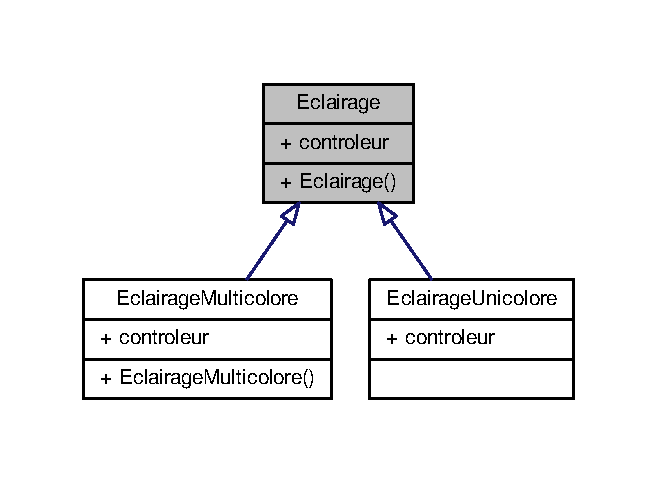
\includegraphics[width=300pt]{classEclairage__inherit__graph}
\end{center}
\end{figure}


Graphe de collaboration de Eclairage\+:\nopagebreak
\begin{figure}[H]
\begin{center}
\leavevmode
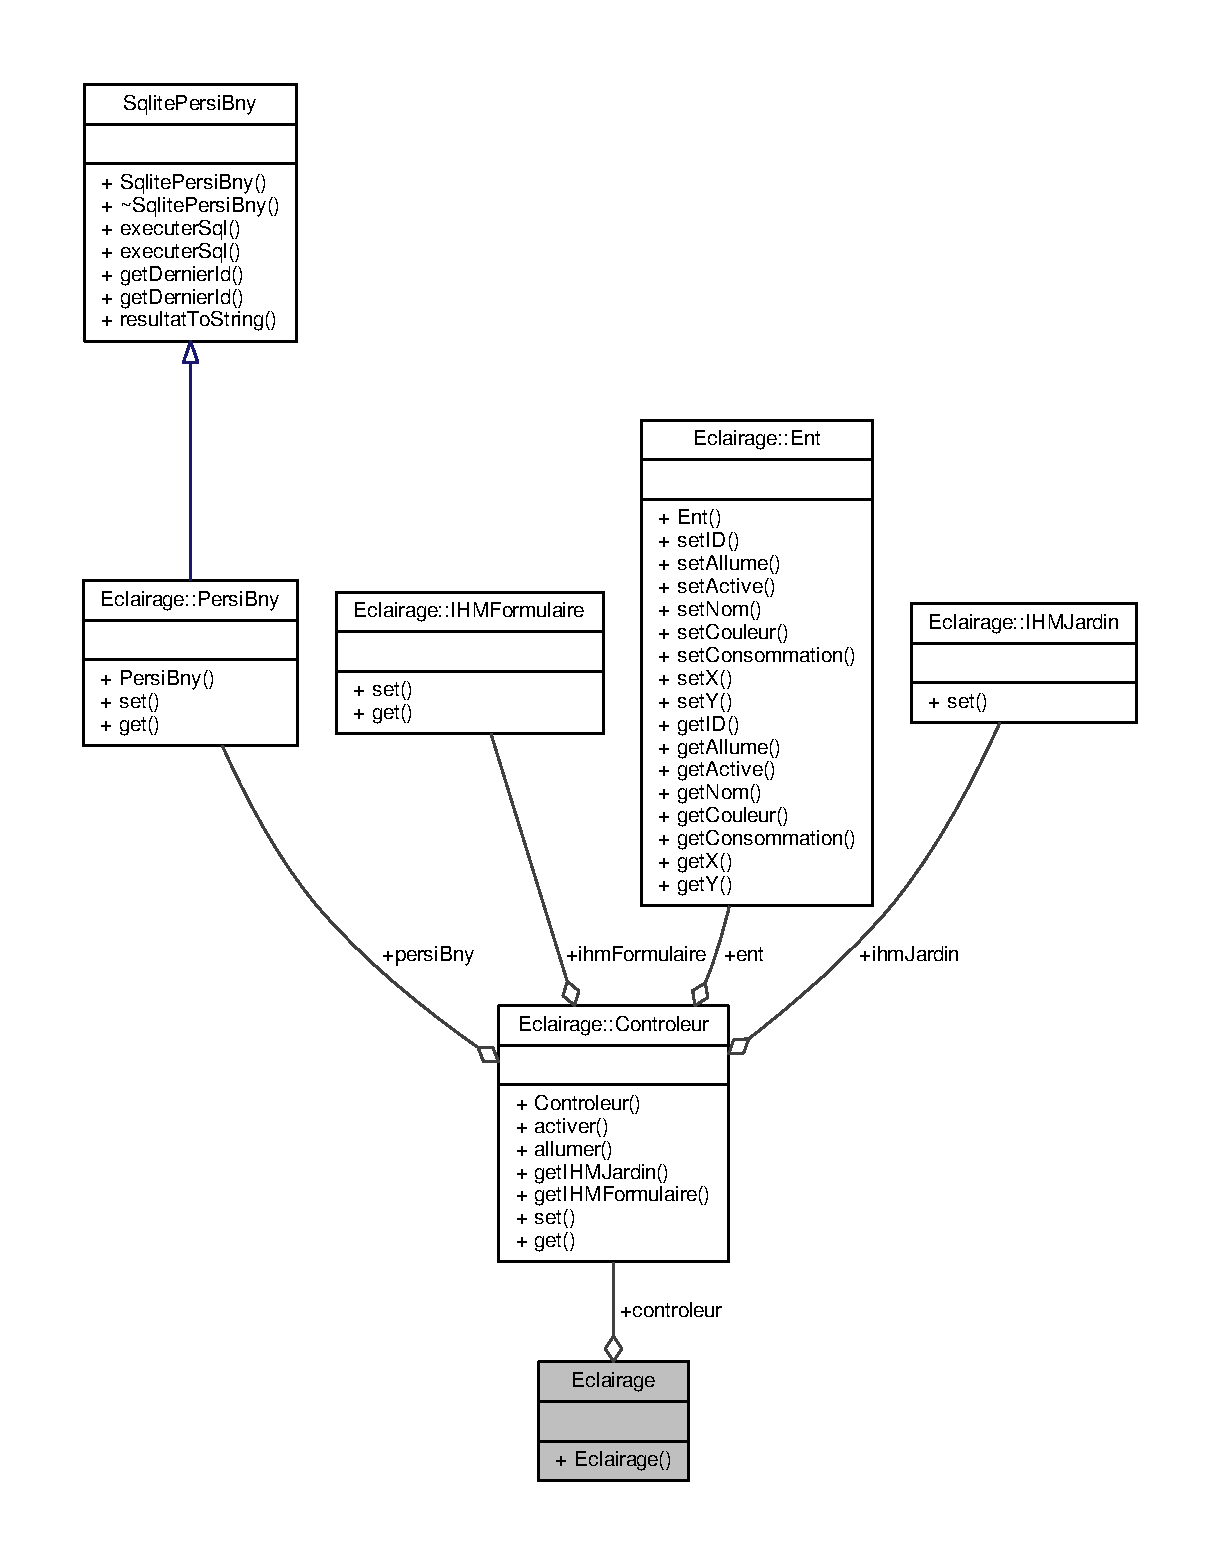
\includegraphics[width=137pt]{classEclairage__coll__graph}
\end{center}
\end{figure}
\subsection*{Classes}
\begin{DoxyCompactItemize}
\item 
class \hyperlink{classEclairage_1_1Controleur}{Controleur}
\item 
class \hyperlink{classEclairage_1_1Ent}{Ent}
\item 
class \hyperlink{classEclairage_1_1IHMFormulaire}{I\+H\+M\+Formulaire}
\item 
class \hyperlink{classEclairage_1_1IHMJardin}{I\+H\+M\+Jardin}
\item 
class \hyperlink{classEclairage_1_1PersiBny}{Persi\+Bny}
\end{DoxyCompactItemize}


\subsection{Description détaillée}
Classe m�re repr�sentant un �clairage g�n�rique comportant\+:
\begin{DoxyItemize}
\item Une I\+HM Formulaire (Forumaire de cr�ation d\textquotesingle{}�clairage)
\item Une I\+HM Jardin (Icone de l\textquotesingle{}eclairage dans l\textquotesingle{}I\+HM de supervision)
\item Un controleur
\item Une entit�
\item Une persistance 
\end{DoxyItemize}

La documentation de cette classe a été générée à partir du fichier suivant \+:\begin{DoxyCompactItemize}
\item 
src/\hyperlink{Eclairage_8h}{Eclairage.\+h}\end{DoxyCompactItemize}

\hypertarget{classEclairageMulticolore_1_1EclairageComBny}{}\section{Référence de la classe Eclairage\+Multicolore\+:\+:Eclairage\+Com\+Bny}
\label{classEclairageMulticolore_1_1EclairageComBny}\index{Eclairage\+Multicolore\+::\+Eclairage\+Com\+Bny@{Eclairage\+Multicolore\+::\+Eclairage\+Com\+Bny}}


{\ttfamily \#include $<$Eclairage\+Multicolore.\+h$>$}



Graphe de collaboration de Eclairage\+Multicolore\+:\+:Eclairage\+Com\+Bny\+:
\nopagebreak
\begin{figure}[H]
\begin{center}
\leavevmode
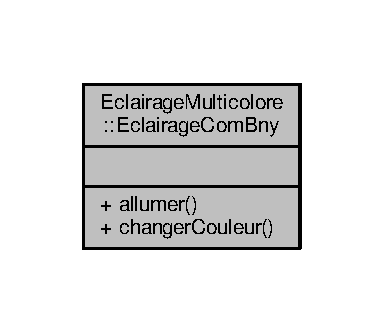
\includegraphics[width=184pt]{classEclairageMulticolore_1_1EclairageComBny__coll__graph}
\end{center}
\end{figure}
\subsection*{Fonctions membres publiques}
\begin{DoxyCompactItemize}
\item 
void \hyperlink{classEclairageMulticolore_1_1EclairageComBny_a863eb83090dc43e4e391098fb568a245}{allumer} (\hyperlink{classEclairageMulticolore_1_1Ent}{Eclairage\+Multicolore\+::\+Ent} \&ent, bool etat)
\item 
void \hyperlink{classEclairageMulticolore_1_1EclairageComBny_a9ebb704e12ce1ca64de3de1110d84e4d}{changer\+Couleur} (\hyperlink{classEclairageMulticolore_1_1Ent}{Eclairage\+Multicolore\+::\+Ent} \&ent, std\+::string couleur)
\end{DoxyCompactItemize}


\subsection{Description détaillée}
Classe permettant de communiquer par r�seau avec l\textquotesingle{}�clairage 

\subsection{Documentation des fonctions membres}
\mbox{\Hypertarget{classEclairageMulticolore_1_1EclairageComBny_a863eb83090dc43e4e391098fb568a245}\label{classEclairageMulticolore_1_1EclairageComBny_a863eb83090dc43e4e391098fb568a245}} 
\index{Eclairage\+Multicolore\+::\+Eclairage\+Com\+Bny@{Eclairage\+Multicolore\+::\+Eclairage\+Com\+Bny}!allumer@{allumer}}
\index{allumer@{allumer}!Eclairage\+Multicolore\+::\+Eclairage\+Com\+Bny@{Eclairage\+Multicolore\+::\+Eclairage\+Com\+Bny}}
\subsubsection{\texorpdfstring{allumer()}{allumer()}}
{\footnotesize\ttfamily void Eclairage\+Multicolore\+::\+Eclairage\+Com\+Bny\+::allumer (\begin{DoxyParamCaption}\item[{\hyperlink{classEclairageMulticolore_1_1Ent}{Eclairage\+Multicolore\+::\+Ent} \&}]{ent,  }\item[{bool}]{etat }\end{DoxyParamCaption})}

M�thode permettant d\textquotesingle{}allumer un �clairage distant par le r�seau 

Références Eclairage\+Multicolore\+::\+Ent\+::get\+Adresse\+I\+P(), et Eclairage\+::\+Ent\+::get\+I\+D().

\mbox{\Hypertarget{classEclairageMulticolore_1_1EclairageComBny_a9ebb704e12ce1ca64de3de1110d84e4d}\label{classEclairageMulticolore_1_1EclairageComBny_a9ebb704e12ce1ca64de3de1110d84e4d}} 
\index{Eclairage\+Multicolore\+::\+Eclairage\+Com\+Bny@{Eclairage\+Multicolore\+::\+Eclairage\+Com\+Bny}!changer\+Couleur@{changer\+Couleur}}
\index{changer\+Couleur@{changer\+Couleur}!Eclairage\+Multicolore\+::\+Eclairage\+Com\+Bny@{Eclairage\+Multicolore\+::\+Eclairage\+Com\+Bny}}
\subsubsection{\texorpdfstring{changer\+Couleur()}{changerCouleur()}}
{\footnotesize\ttfamily void Eclairage\+Multicolore\+::\+Eclairage\+Com\+Bny\+::changer\+Couleur (\begin{DoxyParamCaption}\item[{\hyperlink{classEclairageMulticolore_1_1Ent}{Eclairage\+Multicolore\+::\+Ent} \&}]{ent,  }\item[{std\+::string}]{couleur }\end{DoxyParamCaption})}

M�thode permettant de changer la couleur un �clairage distant par le r�seau 

Références Eclairage\+Multicolore\+::controleur, Eclairage\+Multicolore\+::\+Controleur\+::ent, Eclairage\+Multicolore\+::\+Ent\+::get\+Adresse\+I\+P(), Eclairage\+::\+Ent\+::get\+I\+D(), Eclairage\+Multicolore\+::\+Ent\+::set\+Adresse\+Mac(), et Eclairage\+::\+Ent\+::set\+I\+D().



La documentation de cette classe a été générée à partir des fichiers suivants \+:\begin{DoxyCompactItemize}
\item 
src/\hyperlink{EclairageMulticolore_8h}{Eclairage\+Multicolore.\+h}\item 
src/\hyperlink{EclairageMulticolore_8cpp}{Eclairage\+Multicolore.\+cpp}\end{DoxyCompactItemize}

\hypertarget{classEclairageUnicolore_1_1EclairageComBny}{}\section{Référence de la classe Eclairage\+Unicolore\+:\+:Eclairage\+Com\+Bny}
\label{classEclairageUnicolore_1_1EclairageComBny}\index{Eclairage\+Unicolore\+::\+Eclairage\+Com\+Bny@{Eclairage\+Unicolore\+::\+Eclairage\+Com\+Bny}}


{\ttfamily \#include $<$Eclairage\+Unicolore.\+h$>$}



Graphe de collaboration de Eclairage\+Unicolore\+:\+:Eclairage\+Com\+Bny\+:
\nopagebreak
\begin{figure}[H]
\begin{center}
\leavevmode
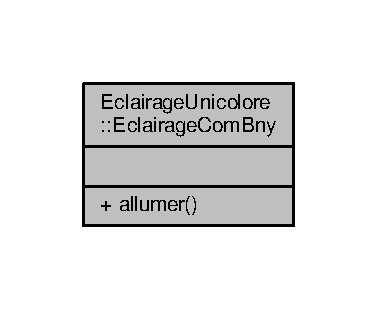
\includegraphics[width=181pt]{classEclairageUnicolore_1_1EclairageComBny__coll__graph}
\end{center}
\end{figure}
\subsection*{Fonctions membres publiques}
\begin{DoxyCompactItemize}
\item 
void \hyperlink{classEclairageUnicolore_1_1EclairageComBny_aba2faf9212f4d7cc1e5d022bdb761a26}{allumer} (\hyperlink{classEclairageUnicolore_1_1Ent}{Eclairage\+Unicolore\+::\+Ent} \&ent, bool etat)
\end{DoxyCompactItemize}


\subsection{Description détaillée}
Classe permettant de communiquer par r�seau avec l\textquotesingle{}�clairage 

\subsection{Documentation des fonctions membres}
\mbox{\Hypertarget{classEclairageUnicolore_1_1EclairageComBny_aba2faf9212f4d7cc1e5d022bdb761a26}\label{classEclairageUnicolore_1_1EclairageComBny_aba2faf9212f4d7cc1e5d022bdb761a26}} 
\index{Eclairage\+Unicolore\+::\+Eclairage\+Com\+Bny@{Eclairage\+Unicolore\+::\+Eclairage\+Com\+Bny}!allumer@{allumer}}
\index{allumer@{allumer}!Eclairage\+Unicolore\+::\+Eclairage\+Com\+Bny@{Eclairage\+Unicolore\+::\+Eclairage\+Com\+Bny}}
\subsubsection{\texorpdfstring{allumer()}{allumer()}}
{\footnotesize\ttfamily void Eclairage\+Unicolore\+::\+Eclairage\+Com\+Bny\+::allumer (\begin{DoxyParamCaption}\item[{\hyperlink{classEclairageUnicolore_1_1Ent}{Eclairage\+Unicolore\+::\+Ent} \&}]{ent,  }\item[{bool}]{etat }\end{DoxyParamCaption})}

M�thode permettant d\textquotesingle{}allumer un �clairage distant par le r�seau 

Références Eclairage\+::\+Ent\+::get\+I\+D(), et main().



La documentation de cette classe a été générée à partir des fichiers suivants \+:\begin{DoxyCompactItemize}
\item 
src/\hyperlink{EclairageUnicolore_8h}{Eclairage\+Unicolore.\+h}\item 
src/\hyperlink{EclairageUnicolore_8cpp}{Eclairage\+Unicolore.\+cpp}\end{DoxyCompactItemize}

\hypertarget{classEclairageMulticolore}{}\section{Référence de la classe Eclairage\+Multicolore}
\label{classEclairageMulticolore}\index{Eclairage\+Multicolore@{Eclairage\+Multicolore}}


{\ttfamily \#include $<$Eclairage\+Multicolore.\+h$>$}



Graphe d\textquotesingle{}héritage de Eclairage\+Multicolore\+:
\nopagebreak
\begin{figure}[H]
\begin{center}
\leavevmode
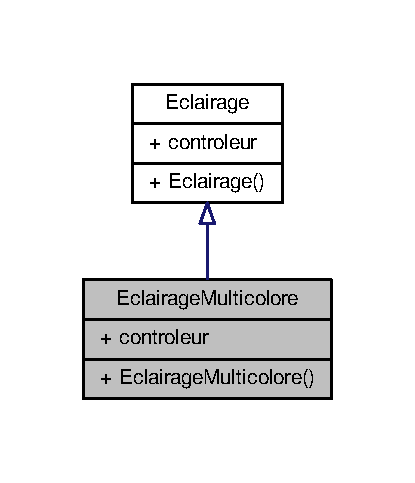
\includegraphics[width=199pt]{classEclairageMulticolore__inherit__graph}
\end{center}
\end{figure}


Graphe de collaboration de Eclairage\+Multicolore\+:
\nopagebreak
\begin{figure}[H]
\begin{center}
\leavevmode
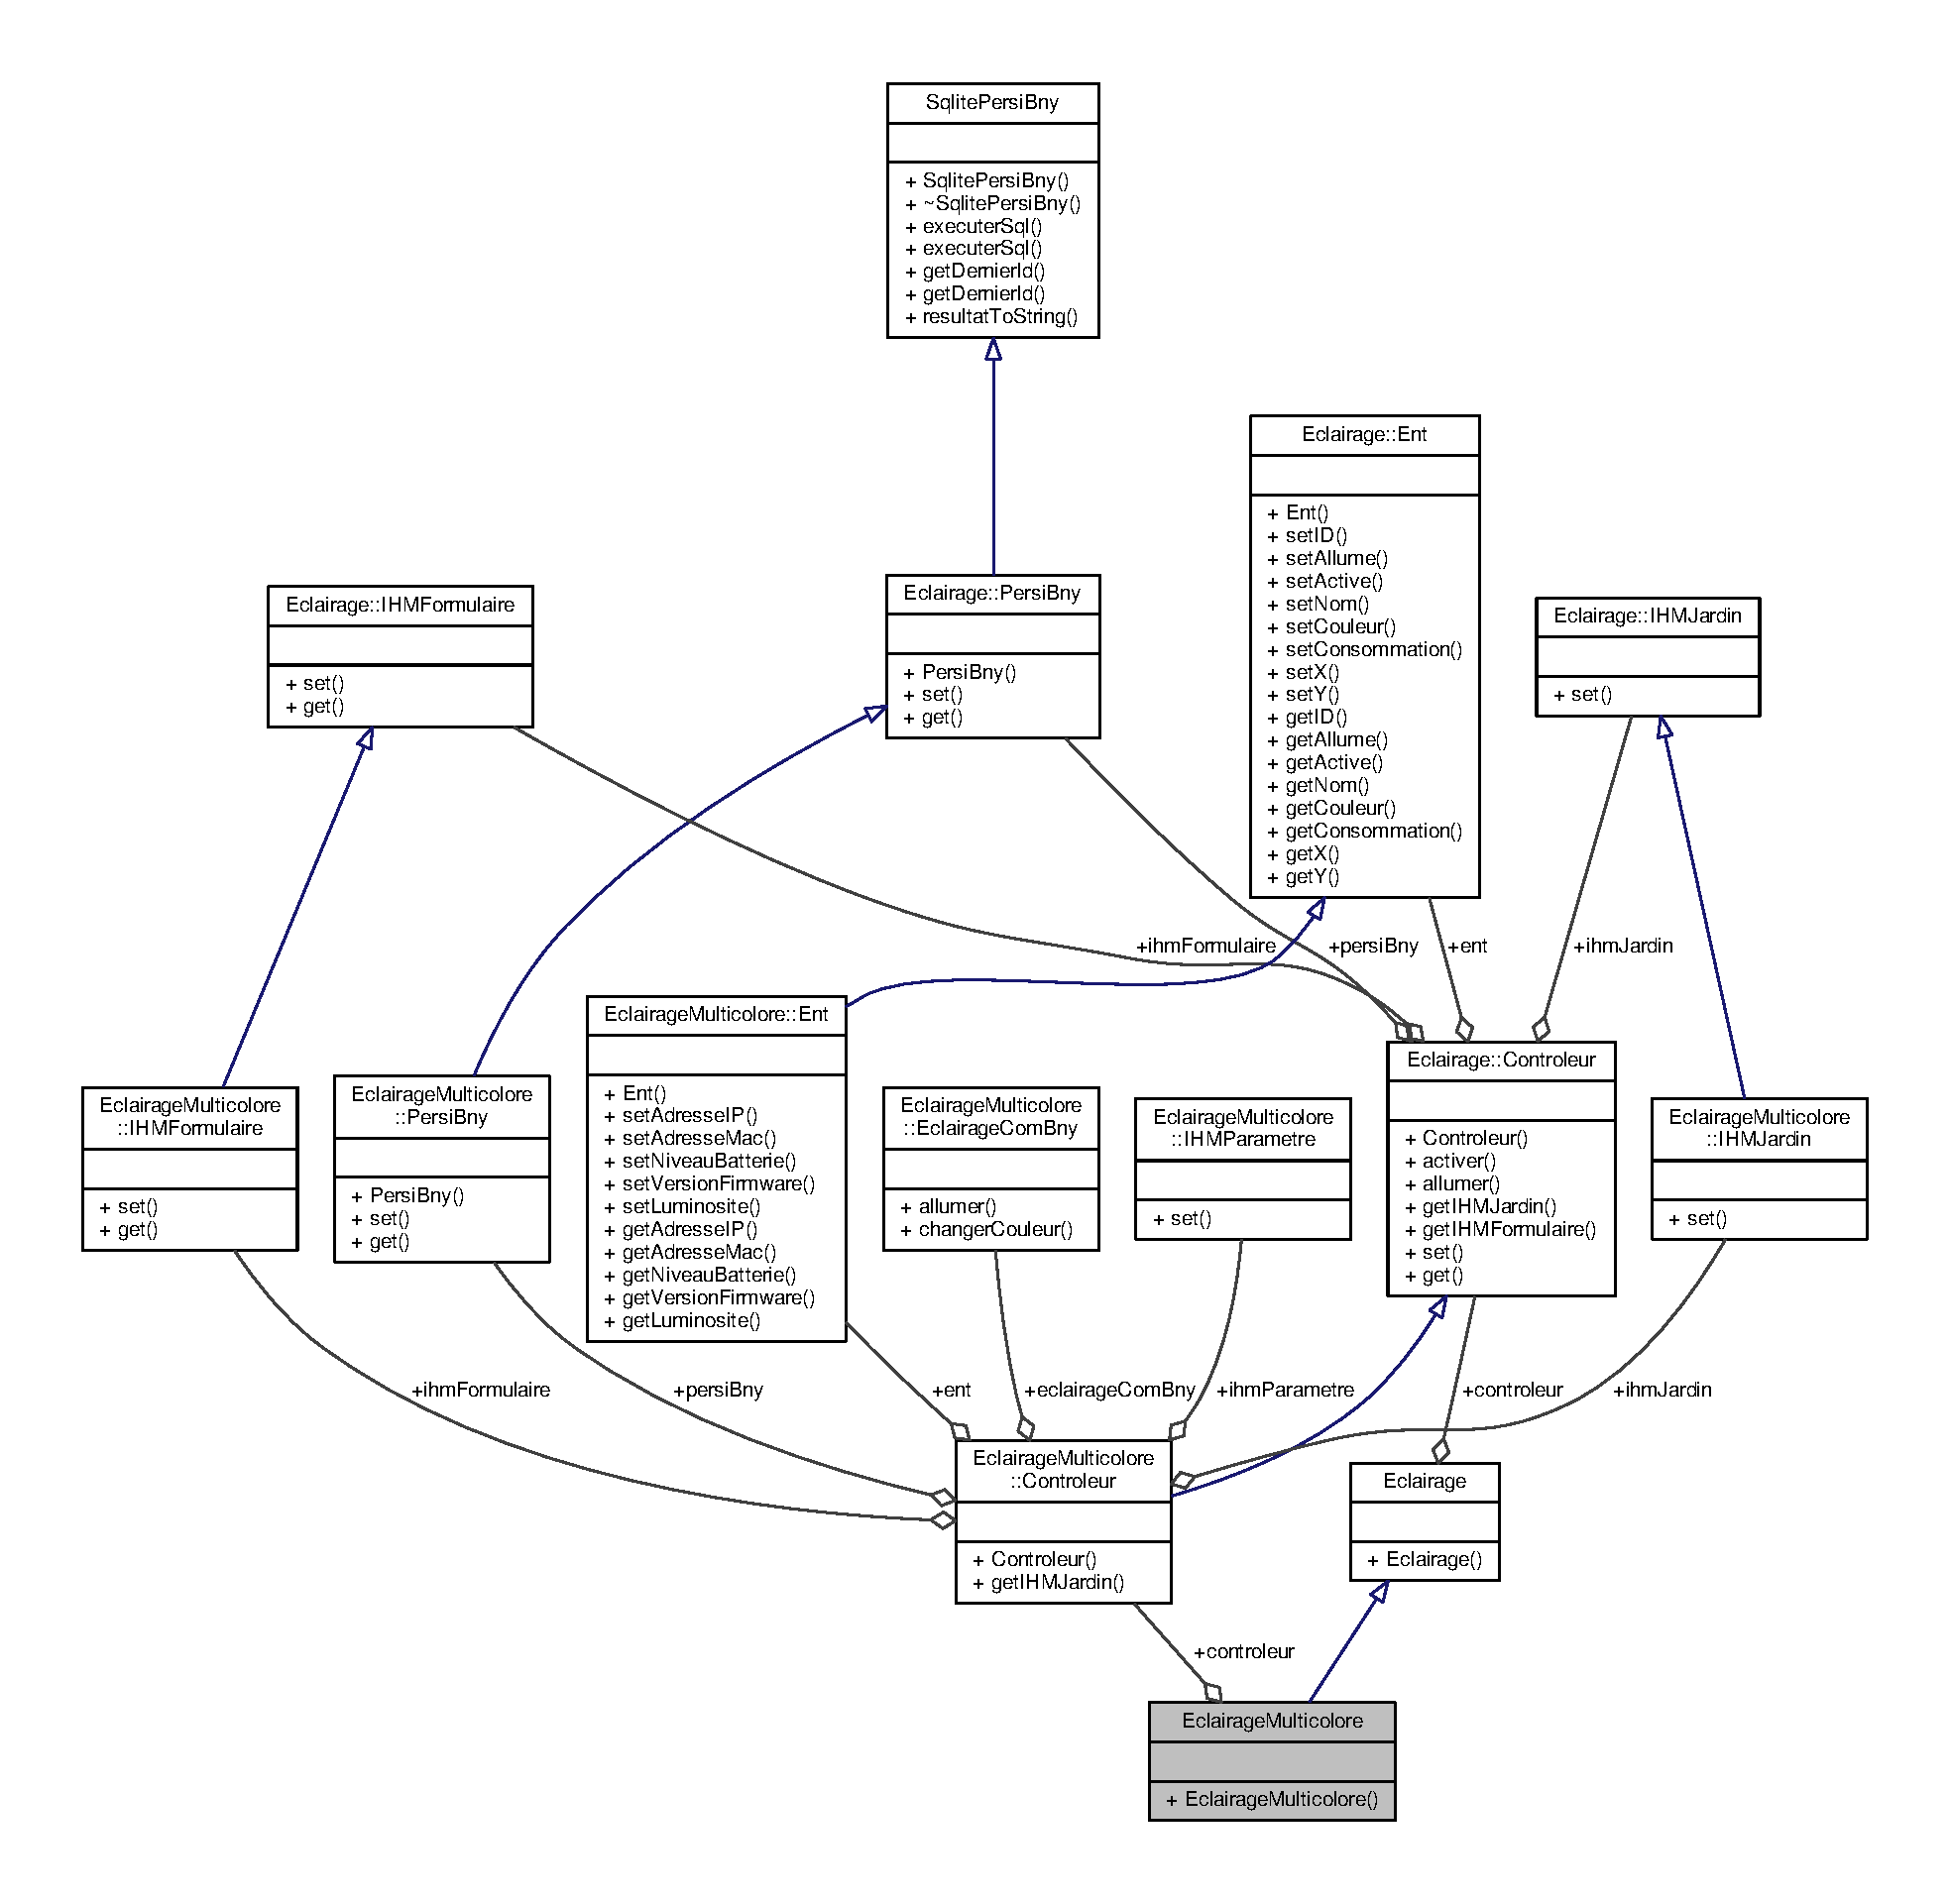
\includegraphics[width=350pt]{classEclairageMulticolore__coll__graph}
\end{center}
\end{figure}
\subsection*{Classes}
\begin{DoxyCompactItemize}
\item 
class \hyperlink{classEclairageMulticolore_1_1Controleur}{Controleur}
\item 
class \hyperlink{classEclairageMulticolore_1_1EclairageComBny}{Eclairage\+Com\+Bny}
\item 
class \hyperlink{classEclairageMulticolore_1_1Ent}{Ent}
\item 
class \hyperlink{classEclairageMulticolore_1_1IHMFormulaire}{I\+H\+M\+Formulaire}
\item 
class \hyperlink{classEclairageMulticolore_1_1IHMJardin}{I\+H\+M\+Jardin}
\item 
class \hyperlink{classEclairageMulticolore_1_1IHMParametre}{I\+H\+M\+Parametre}
\item 
class \hyperlink{classEclairageMulticolore_1_1PersiBny}{Persi\+Bny}
\end{DoxyCompactItemize}
\subsection*{Fonctions membres publiques}
\begin{DoxyCompactItemize}
\item 
\hyperlink{classEclairageMulticolore_a4ed0135965af48317dc414a7af731358}{Eclairage\+Multicolore} ()
\end{DoxyCompactItemize}
\subsection*{Attributs publics}
\begin{DoxyCompactItemize}
\item 
\hyperlink{classEclairageMulticolore_1_1Controleur}{Controleur} \hyperlink{classEclairageMulticolore_a676c67e499fa0883aef82f76ca80a86d}{controleur}
\end{DoxyCompactItemize}


\subsection{Description détaillée}
Classe fille (de eclairage) repr�sentant un �clairage multicolore comportant\+:
\begin{DoxyItemize}
\item Un controleur
\item Une entit� comportant\+:
\begin{DoxyItemize}
\item l\textquotesingle{}adresse IP de l\textquotesingle{}eclairage
\item son adresse M\+AC bluetooth
\item le niveau de sa batterie
\item sa version de firmware
\item le taux de luminosit� actuel
\end{DoxyItemize}
\item Une persistance (polymorph�e) 
\end{DoxyItemize}

\subsection{Documentation des constructeurs et destructeur}
\mbox{\Hypertarget{classEclairageMulticolore_a4ed0135965af48317dc414a7af731358}\label{classEclairageMulticolore_a4ed0135965af48317dc414a7af731358}} 
\index{Eclairage\+Multicolore@{Eclairage\+Multicolore}!Eclairage\+Multicolore@{Eclairage\+Multicolore}}
\index{Eclairage\+Multicolore@{Eclairage\+Multicolore}!Eclairage\+Multicolore@{Eclairage\+Multicolore}}
\subsubsection{\texorpdfstring{Eclairage\+Multicolore()}{EclairageMulticolore()}}
{\footnotesize\ttfamily Eclairage\+Multicolore\+::\+Eclairage\+Multicolore (\begin{DoxyParamCaption}{ }\end{DoxyParamCaption})\hspace{0.3cm}{\ttfamily [inline]}}



\subsection{Documentation des données membres}
\mbox{\Hypertarget{classEclairageMulticolore_a676c67e499fa0883aef82f76ca80a86d}\label{classEclairageMulticolore_a676c67e499fa0883aef82f76ca80a86d}} 
\index{Eclairage\+Multicolore@{Eclairage\+Multicolore}!controleur@{controleur}}
\index{controleur@{controleur}!Eclairage\+Multicolore@{Eclairage\+Multicolore}}
\subsubsection{\texorpdfstring{controleur}{controleur}}
{\footnotesize\ttfamily \hyperlink{classEclairageMulticolore_1_1Controleur}{Controleur} Eclairage\+Multicolore\+::controleur}



La documentation de cette classe a été générée à partir du fichier suivant \+:\begin{DoxyCompactItemize}
\item 
src/\hyperlink{EclairageMulticolore_8h}{Eclairage\+Multicolore.\+h}\end{DoxyCompactItemize}

\hypertarget{classEclairageUnicolore}{}\section{Référence de la classe Eclairage\+Unicolore}
\label{classEclairageUnicolore}\index{Eclairage\+Unicolore@{Eclairage\+Unicolore}}


{\ttfamily \#include $<$Eclairage\+Unicolore.\+h$>$}



Graphe d\textquotesingle{}héritage de Eclairage\+Unicolore\+:\nopagebreak
\begin{figure}[H]
\begin{center}
\leavevmode
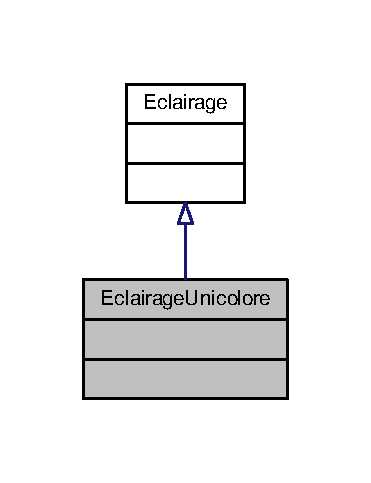
\includegraphics[width=178pt]{classEclairageUnicolore__inherit__graph}
\end{center}
\end{figure}


Graphe de collaboration de Eclairage\+Unicolore\+:\nopagebreak
\begin{figure}[H]
\begin{center}
\leavevmode
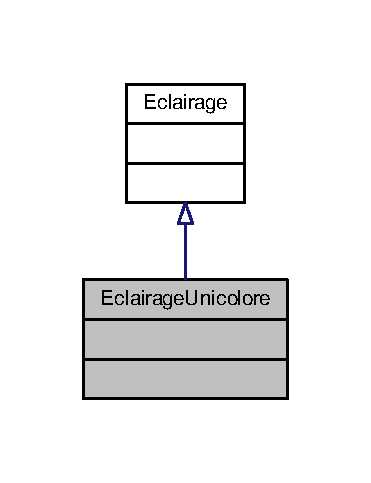
\includegraphics[width=178pt]{classEclairageUnicolore__coll__graph}
\end{center}
\end{figure}
\subsection*{Classes}
\begin{DoxyCompactItemize}
\item 
class \hyperlink{classEclairageUnicolore_1_1Controleur}{Controleur}
\item 
class \hyperlink{classEclairageUnicolore_1_1Ent}{Ent}
\item 
class \hyperlink{classEclairageUnicolore_1_1PersiBny}{Persi\+Bny}
\end{DoxyCompactItemize}


La documentation de cette classe a été générée à partir du fichier suivant \+:\begin{DoxyCompactItemize}
\item 
src/\hyperlink{EclairageUnicolore_8h}{Eclairage\+Unicolore.\+h}\end{DoxyCompactItemize}

\hypertarget{classEclairage_1_1Ent}{}\section{Référence de la classe Eclairage\+:\+:Ent}
\label{classEclairage_1_1Ent}\index{Eclairage\+::\+Ent@{Eclairage\+::\+Ent}}


{\ttfamily \#include $<$Eclairage.\+h$>$}



Graphe d\textquotesingle{}héritage de Eclairage\+:\+:Ent\+:
\nopagebreak
\begin{figure}[H]
\begin{center}
\leavevmode
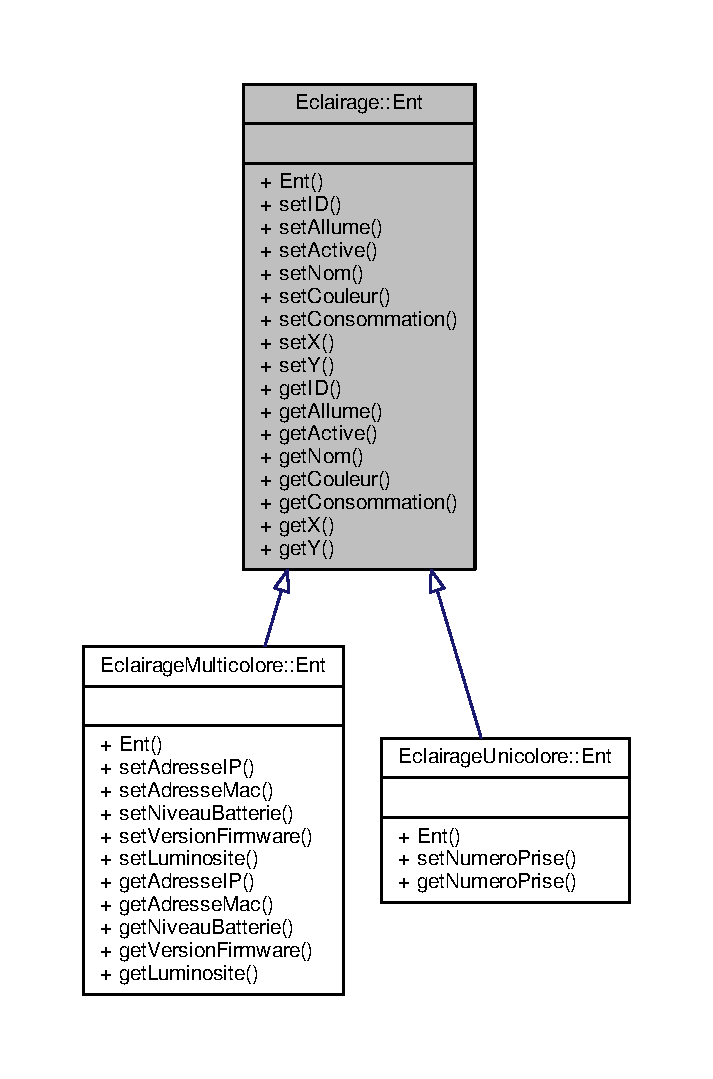
\includegraphics[width=342pt]{classEclairage_1_1Ent__inherit__graph}
\end{center}
\end{figure}


Graphe de collaboration de Eclairage\+:\+:Ent\+:
\nopagebreak
\begin{figure}[H]
\begin{center}
\leavevmode
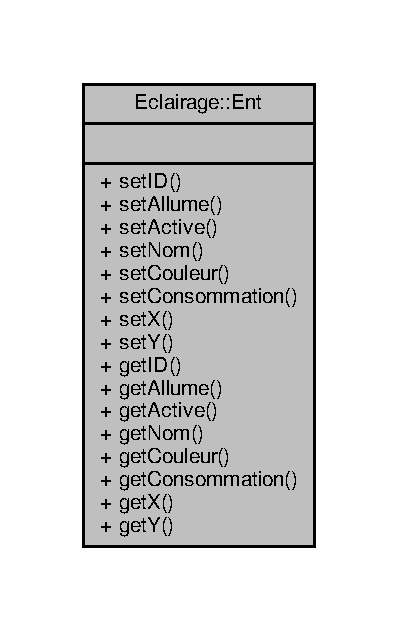
\includegraphics[width=191pt]{classEclairage_1_1Ent__coll__graph}
\end{center}
\end{figure}
\subsection*{Fonctions membres publiques}
\begin{DoxyCompactItemize}
\item 
\hyperlink{classEclairage_1_1Ent_a2c185a5889bd49a541d9e1785b25322a}{Ent} ()
\item 
virtual void \hyperlink{classEclairage_1_1Ent_a927ff132e908bb3e68dab254f6c2ac2d}{set\+ID} (const unsigned int \&id)
\item 
virtual void \hyperlink{classEclairage_1_1Ent_a3c9d21bd3c725857050e39eb449d1ad5}{set\+Allume} (bool etat)
\item 
virtual void \hyperlink{classEclairage_1_1Ent_a1e9471a412f746a2284778c8d9548499}{set\+Active} (bool etat)
\item 
virtual void \hyperlink{classEclairage_1_1Ent_a348836d7b3c2f69f376d63c84ace8e3e}{set\+Nom} (const std\+::string \&nom)
\item 
virtual void \hyperlink{classEclairage_1_1Ent_a4cf307c89bd19221aa2cd338fa2eef7d}{set\+Couleur} (std\+::string couleur)
\item 
virtual void \hyperlink{classEclairage_1_1Ent_a64c03bcbe84186341b0d9f23e91cdfd8}{set\+Consommation} (const unsigned int \&conso)
\item 
virtual void \hyperlink{classEclairage_1_1Ent_a4c5528c086dee2b6c5433c6e103f7eeb}{setX} (int x)
\item 
virtual void \hyperlink{classEclairage_1_1Ent_abdf5e31d5b5788c832b964c3712b7231}{setY} (int y)
\item 
virtual unsigned int \hyperlink{classEclairage_1_1Ent_a503507f6dc76a84b54e22ef21d9f301d}{get\+ID} ()
\item 
virtual bool \hyperlink{classEclairage_1_1Ent_a6d968244e96edee75019717f95dbb1d2}{get\+Allume} ()
\item 
virtual bool \hyperlink{classEclairage_1_1Ent_a7fdf3efdeb7ec2f649a79a1681db6e1e}{get\+Active} ()
\item 
virtual std\+::string \hyperlink{classEclairage_1_1Ent_ae440f0f45ec8f6d11e54c1a0ebe8d5c1}{get\+Nom} ()
\item 
virtual std\+::string \hyperlink{classEclairage_1_1Ent_aab5bf5f43963b1d3918b06f1a8348c7e}{get\+Couleur} ()
\item 
virtual unsigned int \hyperlink{classEclairage_1_1Ent_afb847965b5bcccc415bb169e500656f9}{get\+Consommation} ()
\item 
virtual int \hyperlink{classEclairage_1_1Ent_a0b54632cd5ff1bcb588c4f8527361990}{getX} ()
\item 
virtual int \hyperlink{classEclairage_1_1Ent_a12a54fa5d966278eefc4b035142ade70}{getY} ()
\end{DoxyCompactItemize}


\subsection{Documentation des constructeurs et destructeur}
\mbox{\Hypertarget{classEclairage_1_1Ent_a2c185a5889bd49a541d9e1785b25322a}\label{classEclairage_1_1Ent_a2c185a5889bd49a541d9e1785b25322a}} 
\index{Eclairage\+::\+Ent@{Eclairage\+::\+Ent}!Ent@{Ent}}
\index{Ent@{Ent}!Eclairage\+::\+Ent@{Eclairage\+::\+Ent}}
\subsubsection{\texorpdfstring{Ent()}{Ent()}}
{\footnotesize\ttfamily Eclairage\+::\+Ent\+::\+Ent (\begin{DoxyParamCaption}{ }\end{DoxyParamCaption})\hspace{0.3cm}{\ttfamily [inline]}}



Références get\+Active(), get\+Allume(), get\+Consommation(), get\+Couleur(), get\+I\+D(), get\+Nom(), get\+X(), get\+Y(), set\+Active(), set\+Allume(), set\+Consommation(), set\+Couleur(), set\+I\+D(), set\+Nom(), set\+X(), et set\+Y().



\subsection{Documentation des fonctions membres}
\mbox{\Hypertarget{classEclairage_1_1Ent_a7fdf3efdeb7ec2f649a79a1681db6e1e}\label{classEclairage_1_1Ent_a7fdf3efdeb7ec2f649a79a1681db6e1e}} 
\index{Eclairage\+::\+Ent@{Eclairage\+::\+Ent}!get\+Active@{get\+Active}}
\index{get\+Active@{get\+Active}!Eclairage\+::\+Ent@{Eclairage\+::\+Ent}}
\subsubsection{\texorpdfstring{get\+Active()}{getActive()}}
{\footnotesize\ttfamily bool Eclairage\+::\+Ent\+::get\+Active (\begin{DoxyParamCaption}{ }\end{DoxyParamCaption})\hspace{0.3cm}{\ttfamily [virtual]}}



Références Sqlite\+Persi\+Bny\+::executer\+Sql().

\mbox{\Hypertarget{classEclairage_1_1Ent_a6d968244e96edee75019717f95dbb1d2}\label{classEclairage_1_1Ent_a6d968244e96edee75019717f95dbb1d2}} 
\index{Eclairage\+::\+Ent@{Eclairage\+::\+Ent}!get\+Allume@{get\+Allume}}
\index{get\+Allume@{get\+Allume}!Eclairage\+::\+Ent@{Eclairage\+::\+Ent}}
\subsubsection{\texorpdfstring{get\+Allume()}{getAllume()}}
{\footnotesize\ttfamily bool Eclairage\+::\+Ent\+::get\+Allume (\begin{DoxyParamCaption}{ }\end{DoxyParamCaption})\hspace{0.3cm}{\ttfamily [virtual]}}



Références Sqlite\+Persi\+Bny\+::executer\+Sql().

\mbox{\Hypertarget{classEclairage_1_1Ent_afb847965b5bcccc415bb169e500656f9}\label{classEclairage_1_1Ent_afb847965b5bcccc415bb169e500656f9}} 
\index{Eclairage\+::\+Ent@{Eclairage\+::\+Ent}!get\+Consommation@{get\+Consommation}}
\index{get\+Consommation@{get\+Consommation}!Eclairage\+::\+Ent@{Eclairage\+::\+Ent}}
\subsubsection{\texorpdfstring{get\+Consommation()}{getConsommation()}}
{\footnotesize\ttfamily unsigned int Eclairage\+::\+Ent\+::get\+Consommation (\begin{DoxyParamCaption}{ }\end{DoxyParamCaption})\hspace{0.3cm}{\ttfamily [virtual]}}



Références Sqlite\+Persi\+Bny\+::executer\+Sql().

\mbox{\Hypertarget{classEclairage_1_1Ent_aab5bf5f43963b1d3918b06f1a8348c7e}\label{classEclairage_1_1Ent_aab5bf5f43963b1d3918b06f1a8348c7e}} 
\index{Eclairage\+::\+Ent@{Eclairage\+::\+Ent}!get\+Couleur@{get\+Couleur}}
\index{get\+Couleur@{get\+Couleur}!Eclairage\+::\+Ent@{Eclairage\+::\+Ent}}
\subsubsection{\texorpdfstring{get\+Couleur()}{getCouleur()}}
{\footnotesize\ttfamily std\+::string Eclairage\+::\+Ent\+::get\+Couleur (\begin{DoxyParamCaption}{ }\end{DoxyParamCaption})\hspace{0.3cm}{\ttfamily [virtual]}}



Références Sqlite\+Persi\+Bny\+::executer\+Sql().

\mbox{\Hypertarget{classEclairage_1_1Ent_a503507f6dc76a84b54e22ef21d9f301d}\label{classEclairage_1_1Ent_a503507f6dc76a84b54e22ef21d9f301d}} 
\index{Eclairage\+::\+Ent@{Eclairage\+::\+Ent}!get\+ID@{get\+ID}}
\index{get\+ID@{get\+ID}!Eclairage\+::\+Ent@{Eclairage\+::\+Ent}}
\subsubsection{\texorpdfstring{get\+I\+D()}{getID()}}
{\footnotesize\ttfamily unsigned int Eclairage\+::\+Ent\+::get\+ID (\begin{DoxyParamCaption}{ }\end{DoxyParamCaption})\hspace{0.3cm}{\ttfamily [virtual]}}

\mbox{\Hypertarget{classEclairage_1_1Ent_ae440f0f45ec8f6d11e54c1a0ebe8d5c1}\label{classEclairage_1_1Ent_ae440f0f45ec8f6d11e54c1a0ebe8d5c1}} 
\index{Eclairage\+::\+Ent@{Eclairage\+::\+Ent}!get\+Nom@{get\+Nom}}
\index{get\+Nom@{get\+Nom}!Eclairage\+::\+Ent@{Eclairage\+::\+Ent}}
\subsubsection{\texorpdfstring{get\+Nom()}{getNom()}}
{\footnotesize\ttfamily std\+::string Eclairage\+::\+Ent\+::get\+Nom (\begin{DoxyParamCaption}{ }\end{DoxyParamCaption})\hspace{0.3cm}{\ttfamily [virtual]}}



Références Sqlite\+Persi\+Bny\+::executer\+Sql().

\mbox{\Hypertarget{classEclairage_1_1Ent_a0b54632cd5ff1bcb588c4f8527361990}\label{classEclairage_1_1Ent_a0b54632cd5ff1bcb588c4f8527361990}} 
\index{Eclairage\+::\+Ent@{Eclairage\+::\+Ent}!getX@{getX}}
\index{getX@{getX}!Eclairage\+::\+Ent@{Eclairage\+::\+Ent}}
\subsubsection{\texorpdfstring{get\+X()}{getX()}}
{\footnotesize\ttfamily int Eclairage\+::\+Ent\+::getX (\begin{DoxyParamCaption}{ }\end{DoxyParamCaption})\hspace{0.3cm}{\ttfamily [virtual]}}



Références Sqlite\+Persi\+Bny\+::executer\+Sql().

\mbox{\Hypertarget{classEclairage_1_1Ent_a12a54fa5d966278eefc4b035142ade70}\label{classEclairage_1_1Ent_a12a54fa5d966278eefc4b035142ade70}} 
\index{Eclairage\+::\+Ent@{Eclairage\+::\+Ent}!getY@{getY}}
\index{getY@{getY}!Eclairage\+::\+Ent@{Eclairage\+::\+Ent}}
\subsubsection{\texorpdfstring{get\+Y()}{getY()}}
{\footnotesize\ttfamily int Eclairage\+::\+Ent\+::getY (\begin{DoxyParamCaption}{ }\end{DoxyParamCaption})\hspace{0.3cm}{\ttfamily [virtual]}}



Références Sqlite\+Persi\+Bny\+::executer\+Sql().

\mbox{\Hypertarget{classEclairage_1_1Ent_a1e9471a412f746a2284778c8d9548499}\label{classEclairage_1_1Ent_a1e9471a412f746a2284778c8d9548499}} 
\index{Eclairage\+::\+Ent@{Eclairage\+::\+Ent}!set\+Active@{set\+Active}}
\index{set\+Active@{set\+Active}!Eclairage\+::\+Ent@{Eclairage\+::\+Ent}}
\subsubsection{\texorpdfstring{set\+Active()}{setActive()}}
{\footnotesize\ttfamily void Eclairage\+::\+Ent\+::set\+Active (\begin{DoxyParamCaption}\item[{bool}]{etat }\end{DoxyParamCaption})\hspace{0.3cm}{\ttfamily [virtual]}}



Références Sqlite\+Persi\+Bny\+::executer\+Sql(), et Utility\+::log\+\_\+action().

\mbox{\Hypertarget{classEclairage_1_1Ent_a3c9d21bd3c725857050e39eb449d1ad5}\label{classEclairage_1_1Ent_a3c9d21bd3c725857050e39eb449d1ad5}} 
\index{Eclairage\+::\+Ent@{Eclairage\+::\+Ent}!set\+Allume@{set\+Allume}}
\index{set\+Allume@{set\+Allume}!Eclairage\+::\+Ent@{Eclairage\+::\+Ent}}
\subsubsection{\texorpdfstring{set\+Allume()}{setAllume()}}
{\footnotesize\ttfamily void Eclairage\+::\+Ent\+::set\+Allume (\begin{DoxyParamCaption}\item[{bool}]{etat }\end{DoxyParamCaption})\hspace{0.3cm}{\ttfamily [virtual]}}



Références Sqlite\+Persi\+Bny\+::executer\+Sql(), et Utility\+::log\+\_\+action().

\mbox{\Hypertarget{classEclairage_1_1Ent_a64c03bcbe84186341b0d9f23e91cdfd8}\label{classEclairage_1_1Ent_a64c03bcbe84186341b0d9f23e91cdfd8}} 
\index{Eclairage\+::\+Ent@{Eclairage\+::\+Ent}!set\+Consommation@{set\+Consommation}}
\index{set\+Consommation@{set\+Consommation}!Eclairage\+::\+Ent@{Eclairage\+::\+Ent}}
\subsubsection{\texorpdfstring{set\+Consommation()}{setConsommation()}}
{\footnotesize\ttfamily void Eclairage\+::\+Ent\+::set\+Consommation (\begin{DoxyParamCaption}\item[{const unsigned int \&}]{conso }\end{DoxyParamCaption})\hspace{0.3cm}{\ttfamily [virtual]}}



Références Sqlite\+Persi\+Bny\+::executer\+Sql(), et Utility\+::log\+\_\+action().

\mbox{\Hypertarget{classEclairage_1_1Ent_a4cf307c89bd19221aa2cd338fa2eef7d}\label{classEclairage_1_1Ent_a4cf307c89bd19221aa2cd338fa2eef7d}} 
\index{Eclairage\+::\+Ent@{Eclairage\+::\+Ent}!set\+Couleur@{set\+Couleur}}
\index{set\+Couleur@{set\+Couleur}!Eclairage\+::\+Ent@{Eclairage\+::\+Ent}}
\subsubsection{\texorpdfstring{set\+Couleur()}{setCouleur()}}
{\footnotesize\ttfamily void Eclairage\+::\+Ent\+::set\+Couleur (\begin{DoxyParamCaption}\item[{std\+::string}]{couleur }\end{DoxyParamCaption})\hspace{0.3cm}{\ttfamily [virtual]}}



Références Sqlite\+Persi\+Bny\+::executer\+Sql(), et Utility\+::log\+\_\+action().

\mbox{\Hypertarget{classEclairage_1_1Ent_a927ff132e908bb3e68dab254f6c2ac2d}\label{classEclairage_1_1Ent_a927ff132e908bb3e68dab254f6c2ac2d}} 
\index{Eclairage\+::\+Ent@{Eclairage\+::\+Ent}!set\+ID@{set\+ID}}
\index{set\+ID@{set\+ID}!Eclairage\+::\+Ent@{Eclairage\+::\+Ent}}
\subsubsection{\texorpdfstring{set\+I\+D()}{setID()}}
{\footnotesize\ttfamily void Eclairage\+::\+Ent\+::set\+ID (\begin{DoxyParamCaption}\item[{const unsigned int \&}]{id }\end{DoxyParamCaption})\hspace{0.3cm}{\ttfamily [virtual]}}



Références Sqlite\+Persi\+Bny\+::executer\+Sql().

\mbox{\Hypertarget{classEclairage_1_1Ent_a348836d7b3c2f69f376d63c84ace8e3e}\label{classEclairage_1_1Ent_a348836d7b3c2f69f376d63c84ace8e3e}} 
\index{Eclairage\+::\+Ent@{Eclairage\+::\+Ent}!set\+Nom@{set\+Nom}}
\index{set\+Nom@{set\+Nom}!Eclairage\+::\+Ent@{Eclairage\+::\+Ent}}
\subsubsection{\texorpdfstring{set\+Nom()}{setNom()}}
{\footnotesize\ttfamily void Eclairage\+::\+Ent\+::set\+Nom (\begin{DoxyParamCaption}\item[{const std\+::string \&}]{nom }\end{DoxyParamCaption})\hspace{0.3cm}{\ttfamily [virtual]}}



Références Sqlite\+Persi\+Bny\+::executer\+Sql(), et Utility\+::log\+\_\+action().

\mbox{\Hypertarget{classEclairage_1_1Ent_a4c5528c086dee2b6c5433c6e103f7eeb}\label{classEclairage_1_1Ent_a4c5528c086dee2b6c5433c6e103f7eeb}} 
\index{Eclairage\+::\+Ent@{Eclairage\+::\+Ent}!setX@{setX}}
\index{setX@{setX}!Eclairage\+::\+Ent@{Eclairage\+::\+Ent}}
\subsubsection{\texorpdfstring{set\+X()}{setX()}}
{\footnotesize\ttfamily void Eclairage\+::\+Ent\+::setX (\begin{DoxyParamCaption}\item[{int}]{x }\end{DoxyParamCaption})\hspace{0.3cm}{\ttfamily [virtual]}}



Références Sqlite\+Persi\+Bny\+::executer\+Sql().

\mbox{\Hypertarget{classEclairage_1_1Ent_abdf5e31d5b5788c832b964c3712b7231}\label{classEclairage_1_1Ent_abdf5e31d5b5788c832b964c3712b7231}} 
\index{Eclairage\+::\+Ent@{Eclairage\+::\+Ent}!setY@{setY}}
\index{setY@{setY}!Eclairage\+::\+Ent@{Eclairage\+::\+Ent}}
\subsubsection{\texorpdfstring{set\+Y()}{setY()}}
{\footnotesize\ttfamily void Eclairage\+::\+Ent\+::setY (\begin{DoxyParamCaption}\item[{int}]{y }\end{DoxyParamCaption})\hspace{0.3cm}{\ttfamily [virtual]}}



Références Sqlite\+Persi\+Bny\+::executer\+Sql().



La documentation de cette classe a été générée à partir des fichiers suivants \+:\begin{DoxyCompactItemize}
\item 
src/\hyperlink{Eclairage_8h}{Eclairage.\+h}\item 
src/\hyperlink{Eclairage_8cpp}{Eclairage.\+cpp}\end{DoxyCompactItemize}

\hypertarget{classEclairageMulticolore_1_1Ent}{}\section{Référence de la classe Eclairage\+Multicolore\+:\+:Ent}
\label{classEclairageMulticolore_1_1Ent}\index{Eclairage\+Multicolore\+::\+Ent@{Eclairage\+Multicolore\+::\+Ent}}


{\ttfamily \#include $<$Eclairage\+Multicolore.\+h$>$}



Graphe d\textquotesingle{}héritage de Eclairage\+Multicolore\+:\+:Ent\+:
\nopagebreak
\begin{figure}[H]
\begin{center}
\leavevmode
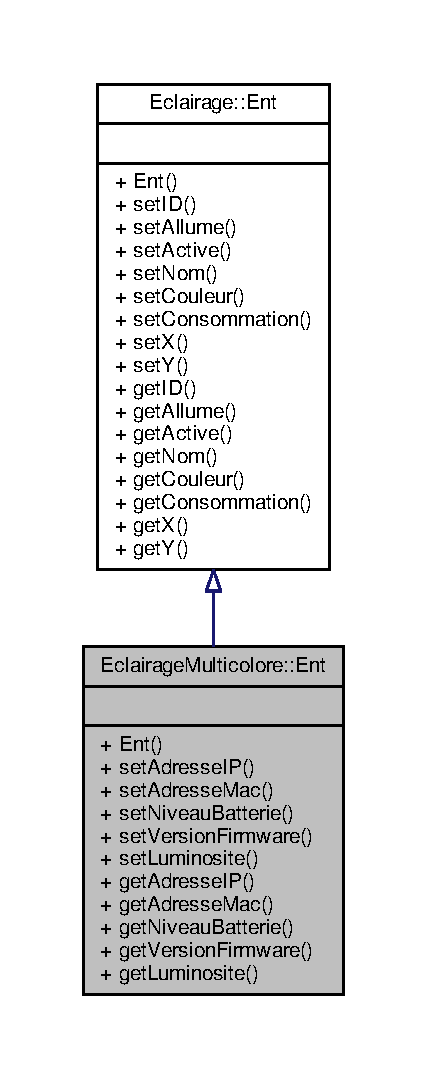
\includegraphics[width=205pt]{classEclairageMulticolore_1_1Ent__inherit__graph}
\end{center}
\end{figure}


Graphe de collaboration de Eclairage\+Multicolore\+:\+:Ent\+:
\nopagebreak
\begin{figure}[H]
\begin{center}
\leavevmode
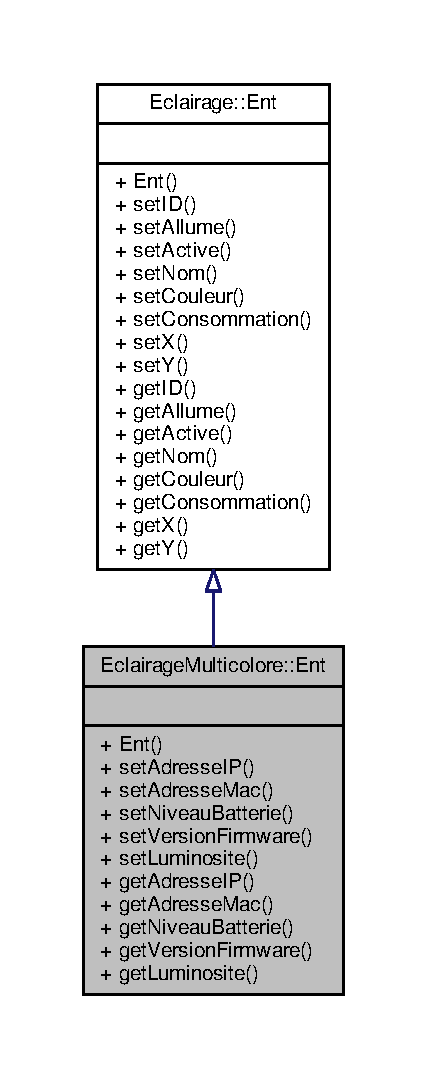
\includegraphics[width=205pt]{classEclairageMulticolore_1_1Ent__coll__graph}
\end{center}
\end{figure}
\subsection*{Fonctions membres publiques}
\begin{DoxyCompactItemize}
\item 
\hyperlink{classEclairageMulticolore_1_1Ent_a1827dfdb3bed2e7d54cfe968594f1554}{Ent} ()
\item 
void \hyperlink{classEclairageMulticolore_1_1Ent_a6078fbeb06a59bf1588fbd091088063a}{set\+Adresse\+IP} (std\+::string adresse\+IP)
\item 
void \hyperlink{classEclairageMulticolore_1_1Ent_a25d7782dfbf10906f9cd2193e3abde74}{set\+Adresse\+Mac} (std\+::string adresse\+Mac)
\item 
void \hyperlink{classEclairageMulticolore_1_1Ent_ab2543b93055678eb150e9840c1263904}{set\+Niveau\+Batterie} (unsigned int niveau\+Batterie)
\item 
void \hyperlink{classEclairageMulticolore_1_1Ent_a8d4b24f6283dad3d1eebd990c32500df}{set\+Version\+Firmware} (float version)
\item 
void \hyperlink{classEclairageMulticolore_1_1Ent_a460390825420ff54e2226ab599ec9192}{set\+Luminosite} (int luminosite)
\item 
std\+::string \hyperlink{classEclairageMulticolore_1_1Ent_ab94fe4fea3e833da751893b042b58c72}{get\+Adresse\+IP} ()
\item 
std\+::string \hyperlink{classEclairageMulticolore_1_1Ent_ae507ad469e0e50b258d949e86e7fc964}{get\+Adresse\+Mac} ()
\item 
unsigned int \hyperlink{classEclairageMulticolore_1_1Ent_ace38da1ad4db26da09187eb9057aa814}{get\+Niveau\+Batterie} ()
\item 
float \hyperlink{classEclairageMulticolore_1_1Ent_a1d3deebf88fdd71633bc92219a070ce1}{get\+Version\+Firmware} ()
\item 
int \hyperlink{classEclairageMulticolore_1_1Ent_a904bd089ddde05670d7390fa609e43a9}{get\+Luminosite} ()
\end{DoxyCompactItemize}


\subsection{Description détaillée}
Classe entit� de l\textquotesingle{}�clairage comportant\+:
\begin{DoxyItemize}
\item Une adresse IP
\end{DoxyItemize}

Un adresse M\+AC
\begin{DoxyItemize}
\item Le niveau de batterie du Rapsberry\+Pi controlant l\textquotesingle{}�clairage
\item La version du firmware
\item La lminosit� venant du capteur sur le R\+PI 
\end{DoxyItemize}

\subsection{Documentation des constructeurs et destructeur}
\mbox{\Hypertarget{classEclairageMulticolore_1_1Ent_a1827dfdb3bed2e7d54cfe968594f1554}\label{classEclairageMulticolore_1_1Ent_a1827dfdb3bed2e7d54cfe968594f1554}} 
\index{Eclairage\+Multicolore\+::\+Ent@{Eclairage\+Multicolore\+::\+Ent}!Ent@{Ent}}
\index{Ent@{Ent}!Eclairage\+Multicolore\+::\+Ent@{Eclairage\+Multicolore\+::\+Ent}}
\subsubsection{\texorpdfstring{Ent()}{Ent()}}
{\footnotesize\ttfamily Eclairage\+Multicolore\+::\+Ent\+::\+Ent (\begin{DoxyParamCaption}{ }\end{DoxyParamCaption})\hspace{0.3cm}{\ttfamily [inline]}}



Références get\+Adresse\+I\+P(), get\+Adresse\+Mac(), get\+Luminosite(), get\+Niveau\+Batterie(), get\+Version\+Firmware(), set\+Adresse\+I\+P(), set\+Adresse\+Mac(), set\+Luminosite(), set\+Niveau\+Batterie(), et set\+Version\+Firmware().



\subsection{Documentation des fonctions membres}
\mbox{\Hypertarget{classEclairageMulticolore_1_1Ent_ab94fe4fea3e833da751893b042b58c72}\label{classEclairageMulticolore_1_1Ent_ab94fe4fea3e833da751893b042b58c72}} 
\index{Eclairage\+Multicolore\+::\+Ent@{Eclairage\+Multicolore\+::\+Ent}!get\+Adresse\+IP@{get\+Adresse\+IP}}
\index{get\+Adresse\+IP@{get\+Adresse\+IP}!Eclairage\+Multicolore\+::\+Ent@{Eclairage\+Multicolore\+::\+Ent}}
\subsubsection{\texorpdfstring{get\+Adresse\+I\+P()}{getAdresseIP()}}
{\footnotesize\ttfamily std\+::string Eclairage\+Multicolore\+::\+Ent\+::get\+Adresse\+IP (\begin{DoxyParamCaption}{ }\end{DoxyParamCaption})}



Références Sqlite\+Persi\+Bny\+::executer\+Sql().

\mbox{\Hypertarget{classEclairageMulticolore_1_1Ent_ae507ad469e0e50b258d949e86e7fc964}\label{classEclairageMulticolore_1_1Ent_ae507ad469e0e50b258d949e86e7fc964}} 
\index{Eclairage\+Multicolore\+::\+Ent@{Eclairage\+Multicolore\+::\+Ent}!get\+Adresse\+Mac@{get\+Adresse\+Mac}}
\index{get\+Adresse\+Mac@{get\+Adresse\+Mac}!Eclairage\+Multicolore\+::\+Ent@{Eclairage\+Multicolore\+::\+Ent}}
\subsubsection{\texorpdfstring{get\+Adresse\+Mac()}{getAdresseMac()}}
{\footnotesize\ttfamily std\+::string Eclairage\+Multicolore\+::\+Ent\+::get\+Adresse\+Mac (\begin{DoxyParamCaption}{ }\end{DoxyParamCaption})}



Références Sqlite\+Persi\+Bny\+::executer\+Sql().

\mbox{\Hypertarget{classEclairageMulticolore_1_1Ent_a904bd089ddde05670d7390fa609e43a9}\label{classEclairageMulticolore_1_1Ent_a904bd089ddde05670d7390fa609e43a9}} 
\index{Eclairage\+Multicolore\+::\+Ent@{Eclairage\+Multicolore\+::\+Ent}!get\+Luminosite@{get\+Luminosite}}
\index{get\+Luminosite@{get\+Luminosite}!Eclairage\+Multicolore\+::\+Ent@{Eclairage\+Multicolore\+::\+Ent}}
\subsubsection{\texorpdfstring{get\+Luminosite()}{getLuminosite()}}
{\footnotesize\ttfamily int Eclairage\+Multicolore\+::\+Ent\+::get\+Luminosite (\begin{DoxyParamCaption}{ }\end{DoxyParamCaption})}



Références Sqlite\+Persi\+Bny\+::executer\+Sql().

\mbox{\Hypertarget{classEclairageMulticolore_1_1Ent_ace38da1ad4db26da09187eb9057aa814}\label{classEclairageMulticolore_1_1Ent_ace38da1ad4db26da09187eb9057aa814}} 
\index{Eclairage\+Multicolore\+::\+Ent@{Eclairage\+Multicolore\+::\+Ent}!get\+Niveau\+Batterie@{get\+Niveau\+Batterie}}
\index{get\+Niveau\+Batterie@{get\+Niveau\+Batterie}!Eclairage\+Multicolore\+::\+Ent@{Eclairage\+Multicolore\+::\+Ent}}
\subsubsection{\texorpdfstring{get\+Niveau\+Batterie()}{getNiveauBatterie()}}
{\footnotesize\ttfamily unsigned int Eclairage\+Multicolore\+::\+Ent\+::get\+Niveau\+Batterie (\begin{DoxyParamCaption}{ }\end{DoxyParamCaption})}



Références Sqlite\+Persi\+Bny\+::executer\+Sql().

\mbox{\Hypertarget{classEclairageMulticolore_1_1Ent_a1d3deebf88fdd71633bc92219a070ce1}\label{classEclairageMulticolore_1_1Ent_a1d3deebf88fdd71633bc92219a070ce1}} 
\index{Eclairage\+Multicolore\+::\+Ent@{Eclairage\+Multicolore\+::\+Ent}!get\+Version\+Firmware@{get\+Version\+Firmware}}
\index{get\+Version\+Firmware@{get\+Version\+Firmware}!Eclairage\+Multicolore\+::\+Ent@{Eclairage\+Multicolore\+::\+Ent}}
\subsubsection{\texorpdfstring{get\+Version\+Firmware()}{getVersionFirmware()}}
{\footnotesize\ttfamily float Eclairage\+Multicolore\+::\+Ent\+::get\+Version\+Firmware (\begin{DoxyParamCaption}{ }\end{DoxyParamCaption})}



Références Sqlite\+Persi\+Bny\+::executer\+Sql().

\mbox{\Hypertarget{classEclairageMulticolore_1_1Ent_a6078fbeb06a59bf1588fbd091088063a}\label{classEclairageMulticolore_1_1Ent_a6078fbeb06a59bf1588fbd091088063a}} 
\index{Eclairage\+Multicolore\+::\+Ent@{Eclairage\+Multicolore\+::\+Ent}!set\+Adresse\+IP@{set\+Adresse\+IP}}
\index{set\+Adresse\+IP@{set\+Adresse\+IP}!Eclairage\+Multicolore\+::\+Ent@{Eclairage\+Multicolore\+::\+Ent}}
\subsubsection{\texorpdfstring{set\+Adresse\+I\+P()}{setAdresseIP()}}
{\footnotesize\ttfamily void Eclairage\+Multicolore\+::\+Ent\+::set\+Adresse\+IP (\begin{DoxyParamCaption}\item[{std\+::string}]{adresse\+IP }\end{DoxyParamCaption})}



Références Sqlite\+Persi\+Bny\+::executer\+Sql().

\mbox{\Hypertarget{classEclairageMulticolore_1_1Ent_a25d7782dfbf10906f9cd2193e3abde74}\label{classEclairageMulticolore_1_1Ent_a25d7782dfbf10906f9cd2193e3abde74}} 
\index{Eclairage\+Multicolore\+::\+Ent@{Eclairage\+Multicolore\+::\+Ent}!set\+Adresse\+Mac@{set\+Adresse\+Mac}}
\index{set\+Adresse\+Mac@{set\+Adresse\+Mac}!Eclairage\+Multicolore\+::\+Ent@{Eclairage\+Multicolore\+::\+Ent}}
\subsubsection{\texorpdfstring{set\+Adresse\+Mac()}{setAdresseMac()}}
{\footnotesize\ttfamily void Eclairage\+Multicolore\+::\+Ent\+::set\+Adresse\+Mac (\begin{DoxyParamCaption}\item[{std\+::string}]{adresse\+Mac }\end{DoxyParamCaption})}



Références Sqlite\+Persi\+Bny\+::executer\+Sql().

\mbox{\Hypertarget{classEclairageMulticolore_1_1Ent_a460390825420ff54e2226ab599ec9192}\label{classEclairageMulticolore_1_1Ent_a460390825420ff54e2226ab599ec9192}} 
\index{Eclairage\+Multicolore\+::\+Ent@{Eclairage\+Multicolore\+::\+Ent}!set\+Luminosite@{set\+Luminosite}}
\index{set\+Luminosite@{set\+Luminosite}!Eclairage\+Multicolore\+::\+Ent@{Eclairage\+Multicolore\+::\+Ent}}
\subsubsection{\texorpdfstring{set\+Luminosite()}{setLuminosite()}}
{\footnotesize\ttfamily void Eclairage\+Multicolore\+::\+Ent\+::set\+Luminosite (\begin{DoxyParamCaption}\item[{int}]{luminosite }\end{DoxyParamCaption})}



Références Sqlite\+Persi\+Bny\+::executer\+Sql().

\mbox{\Hypertarget{classEclairageMulticolore_1_1Ent_ab2543b93055678eb150e9840c1263904}\label{classEclairageMulticolore_1_1Ent_ab2543b93055678eb150e9840c1263904}} 
\index{Eclairage\+Multicolore\+::\+Ent@{Eclairage\+Multicolore\+::\+Ent}!set\+Niveau\+Batterie@{set\+Niveau\+Batterie}}
\index{set\+Niveau\+Batterie@{set\+Niveau\+Batterie}!Eclairage\+Multicolore\+::\+Ent@{Eclairage\+Multicolore\+::\+Ent}}
\subsubsection{\texorpdfstring{set\+Niveau\+Batterie()}{setNiveauBatterie()}}
{\footnotesize\ttfamily void Eclairage\+Multicolore\+::\+Ent\+::set\+Niveau\+Batterie (\begin{DoxyParamCaption}\item[{unsigned int}]{niveau\+Batterie }\end{DoxyParamCaption})}



Références Sqlite\+Persi\+Bny\+::executer\+Sql().

\mbox{\Hypertarget{classEclairageMulticolore_1_1Ent_a8d4b24f6283dad3d1eebd990c32500df}\label{classEclairageMulticolore_1_1Ent_a8d4b24f6283dad3d1eebd990c32500df}} 
\index{Eclairage\+Multicolore\+::\+Ent@{Eclairage\+Multicolore\+::\+Ent}!set\+Version\+Firmware@{set\+Version\+Firmware}}
\index{set\+Version\+Firmware@{set\+Version\+Firmware}!Eclairage\+Multicolore\+::\+Ent@{Eclairage\+Multicolore\+::\+Ent}}
\subsubsection{\texorpdfstring{set\+Version\+Firmware()}{setVersionFirmware()}}
{\footnotesize\ttfamily void Eclairage\+Multicolore\+::\+Ent\+::set\+Version\+Firmware (\begin{DoxyParamCaption}\item[{float}]{version }\end{DoxyParamCaption})}



Références Sqlite\+Persi\+Bny\+::executer\+Sql().



La documentation de cette classe a été générée à partir des fichiers suivants \+:\begin{DoxyCompactItemize}
\item 
src/\hyperlink{EclairageMulticolore_8h}{Eclairage\+Multicolore.\+h}\item 
src/\hyperlink{EclairageMulticolore_8cpp}{Eclairage\+Multicolore.\+cpp}\end{DoxyCompactItemize}

\hypertarget{classEclairageUnicolore_1_1Ent}{}\section{Référence de la classe Eclairage\+Unicolore\+:\+:Ent}
\label{classEclairageUnicolore_1_1Ent}\index{Eclairage\+Unicolore\+::\+Ent@{Eclairage\+Unicolore\+::\+Ent}}


{\ttfamily \#include $<$Eclairage\+Unicolore.\+h$>$}



Graphe d\textquotesingle{}héritage de Eclairage\+Unicolore\+:\+:Ent\+:
\nopagebreak
\begin{figure}[H]
\begin{center}
\leavevmode
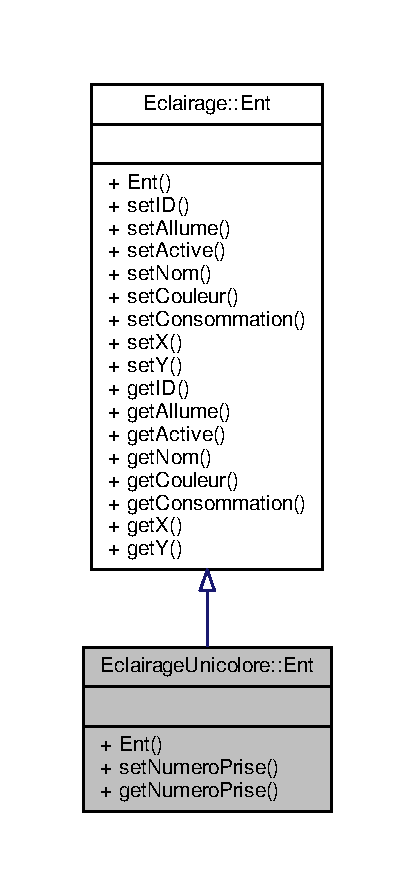
\includegraphics[width=199pt]{classEclairageUnicolore_1_1Ent__inherit__graph}
\end{center}
\end{figure}


Graphe de collaboration de Eclairage\+Unicolore\+:\+:Ent\+:
\nopagebreak
\begin{figure}[H]
\begin{center}
\leavevmode
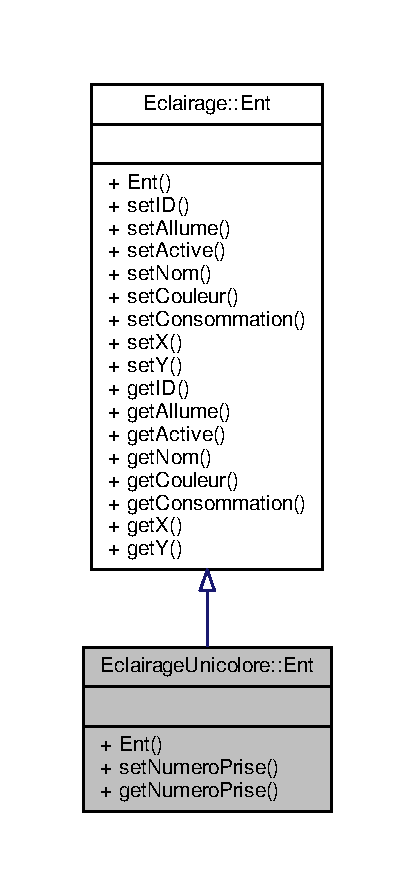
\includegraphics[width=199pt]{classEclairageUnicolore_1_1Ent__coll__graph}
\end{center}
\end{figure}
\subsection*{Fonctions membres publiques}
\begin{DoxyCompactItemize}
\item 
\hyperlink{classEclairageUnicolore_1_1Ent_a0d1e73af143c3cd2e94d01e287ef0a09}{Ent} ()
\item 
void \hyperlink{classEclairageUnicolore_1_1Ent_a641deab83484aed1c93d440da2cb27b1}{set\+Numero\+Prise} (int num)
\item 
int \hyperlink{classEclairageUnicolore_1_1Ent_ad2c1808857d49daaddea050083d8ff9f}{get\+Numero\+Prise} ()
\end{DoxyCompactItemize}


\subsection{Documentation des constructeurs et destructeur}
\mbox{\Hypertarget{classEclairageUnicolore_1_1Ent_a0d1e73af143c3cd2e94d01e287ef0a09}\label{classEclairageUnicolore_1_1Ent_a0d1e73af143c3cd2e94d01e287ef0a09}} 
\index{Eclairage\+Unicolore\+::\+Ent@{Eclairage\+Unicolore\+::\+Ent}!Ent@{Ent}}
\index{Ent@{Ent}!Eclairage\+Unicolore\+::\+Ent@{Eclairage\+Unicolore\+::\+Ent}}
\subsubsection{\texorpdfstring{Ent()}{Ent()}}
{\footnotesize\ttfamily Eclairage\+Unicolore\+::\+Ent\+::\+Ent (\begin{DoxyParamCaption}{ }\end{DoxyParamCaption})\hspace{0.3cm}{\ttfamily [inline]}}



Références get\+Numero\+Prise(), et set\+Numero\+Prise().



\subsection{Documentation des fonctions membres}
\mbox{\Hypertarget{classEclairageUnicolore_1_1Ent_ad2c1808857d49daaddea050083d8ff9f}\label{classEclairageUnicolore_1_1Ent_ad2c1808857d49daaddea050083d8ff9f}} 
\index{Eclairage\+Unicolore\+::\+Ent@{Eclairage\+Unicolore\+::\+Ent}!get\+Numero\+Prise@{get\+Numero\+Prise}}
\index{get\+Numero\+Prise@{get\+Numero\+Prise}!Eclairage\+Unicolore\+::\+Ent@{Eclairage\+Unicolore\+::\+Ent}}
\subsubsection{\texorpdfstring{get\+Numero\+Prise()}{getNumeroPrise()}}
{\footnotesize\ttfamily int Eclairage\+Unicolore\+::\+Ent\+::get\+Numero\+Prise (\begin{DoxyParamCaption}{ }\end{DoxyParamCaption})}

M�thode permettant de r�cup�rer le num�ro de la prise associ� � l\textquotesingle{}�clairage. 

Références Sqlite\+Persi\+Bny\+::executer\+Sql().

\mbox{\Hypertarget{classEclairageUnicolore_1_1Ent_a641deab83484aed1c93d440da2cb27b1}\label{classEclairageUnicolore_1_1Ent_a641deab83484aed1c93d440da2cb27b1}} 
\index{Eclairage\+Unicolore\+::\+Ent@{Eclairage\+Unicolore\+::\+Ent}!set\+Numero\+Prise@{set\+Numero\+Prise}}
\index{set\+Numero\+Prise@{set\+Numero\+Prise}!Eclairage\+Unicolore\+::\+Ent@{Eclairage\+Unicolore\+::\+Ent}}
\subsubsection{\texorpdfstring{set\+Numero\+Prise()}{setNumeroPrise()}}
{\footnotesize\ttfamily void Eclairage\+Unicolore\+::\+Ent\+::set\+Numero\+Prise (\begin{DoxyParamCaption}\item[{int}]{num }\end{DoxyParamCaption})}

M�thode permettant de modifier le numero de la prise associ� � l\textquotesingle{}�clairage. 

Références Sqlite\+Persi\+Bny\+::executer\+Sql(), et Utility\+::log\+\_\+action().



La documentation de cette classe a été générée à partir des fichiers suivants \+:\begin{DoxyCompactItemize}
\item 
src/\hyperlink{EclairageUnicolore_8h}{Eclairage\+Unicolore.\+h}\item 
src/\hyperlink{EclairageUnicolore_8cpp}{Eclairage\+Unicolore.\+cpp}\end{DoxyCompactItemize}

\hypertarget{classFichierTextePersiBny}{}\section{Référence de la classe Fichier\+Texte\+Persi\+Bny}
\label{classFichierTextePersiBny}\index{Fichier\+Texte\+Persi\+Bny@{Fichier\+Texte\+Persi\+Bny}}


{\ttfamily \#include $<$Fichier\+Texte\+Persi\+Bny.\+h$>$}



Graphe d\textquotesingle{}héritage de Fichier\+Texte\+Persi\+Bny\+:
\nopagebreak
\begin{figure}[H]
\begin{center}
\leavevmode
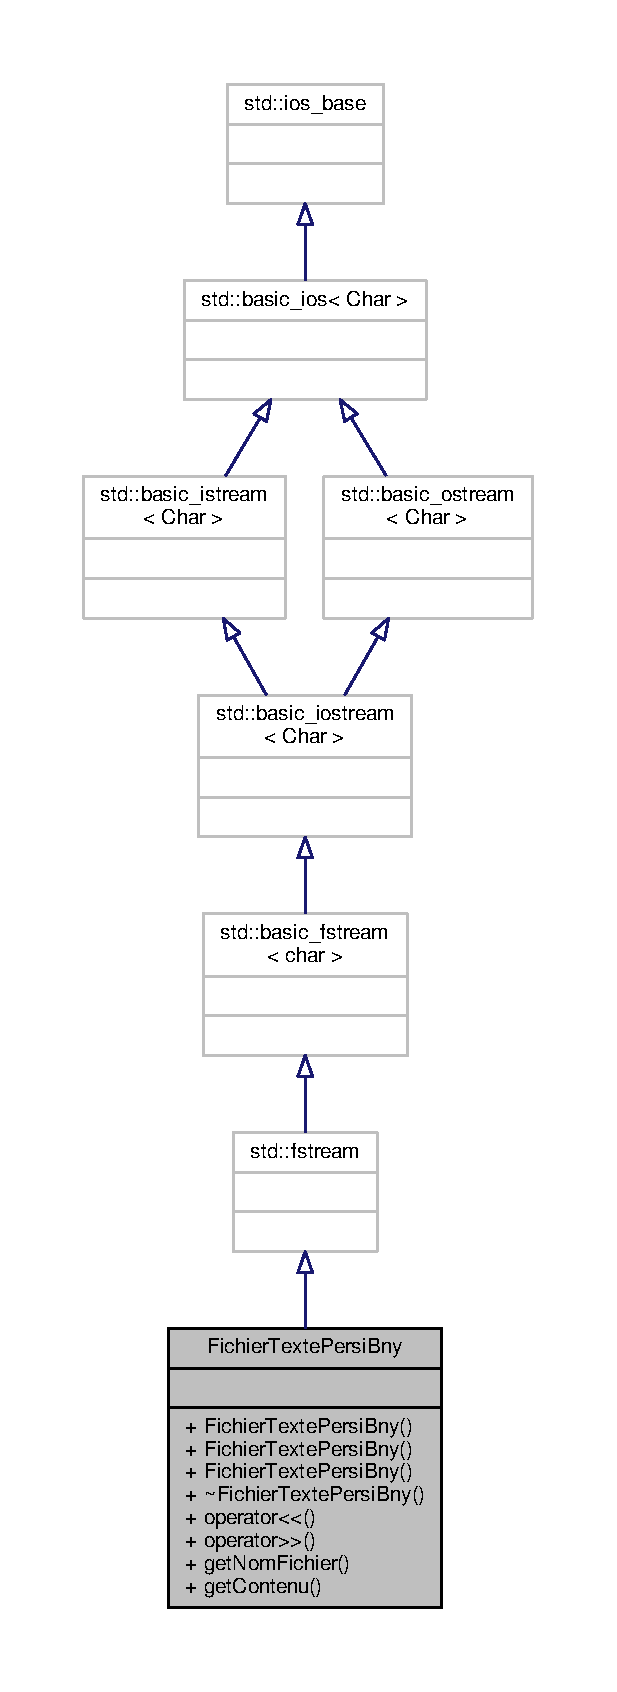
\includegraphics[height=550pt]{classFichierTextePersiBny__inherit__graph}
\end{center}
\end{figure}


Graphe de collaboration de Fichier\+Texte\+Persi\+Bny\+:
\nopagebreak
\begin{figure}[H]
\begin{center}
\leavevmode
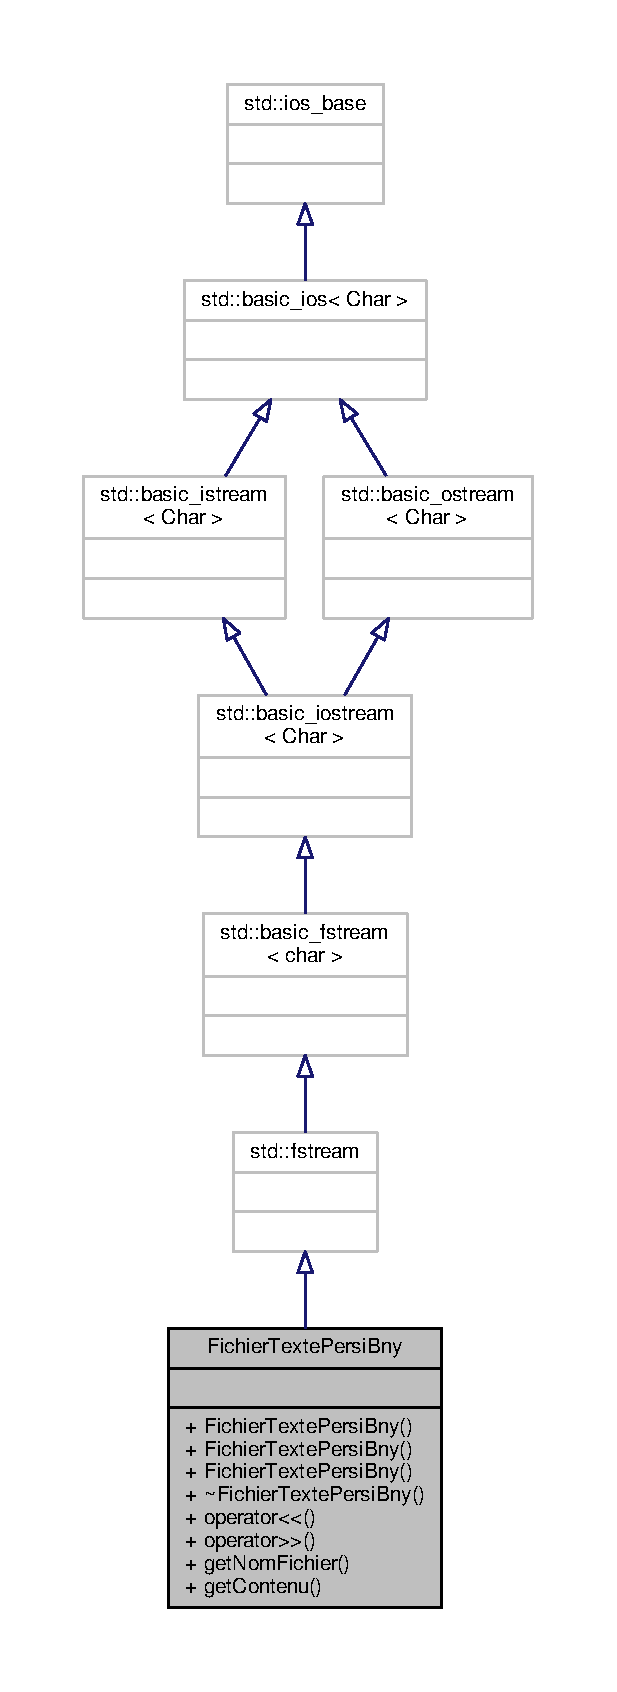
\includegraphics[height=550pt]{classFichierTextePersiBny__coll__graph}
\end{center}
\end{figure}
\subsection*{Fonctions membres publiques}
\begin{DoxyCompactItemize}
\item 
\hyperlink{classFichierTextePersiBny_a6abeffa179773c3d7c00cf53a96019ad}{Fichier\+Texte\+Persi\+Bny} (const char $\ast$nom\+Fichier)
\item 
\hyperlink{classFichierTextePersiBny_a5106857b382a6a576be4f32af29e3b8f}{Fichier\+Texte\+Persi\+Bny} (const std\+::string nom\+Fichier)
\item 
\hyperlink{classFichierTextePersiBny_ac568130ed7a355bd74786f64fff587f2}{Fichier\+Texte\+Persi\+Bny} ()
\item 
\hyperlink{classFichierTextePersiBny_a1ee8d139d3e42d7bcc6b5853f25cb09b}{$\sim$\+Fichier\+Texte\+Persi\+Bny} ()
\item 
{\footnotesize template$<$typename T $>$ }\\\hyperlink{classFichierTextePersiBny}{Fichier\+Texte\+Persi\+Bny} \& \hyperlink{classFichierTextePersiBny_aec7709f80844eb19d021d9633dd6fc4c}{operator$<$$<$} (const T \&data)
\item 
{\footnotesize template$<$typename T $>$ }\\\hyperlink{classFichierTextePersiBny}{Fichier\+Texte\+Persi\+Bny} \& \hyperlink{classFichierTextePersiBny_a06cacad4ff051e5f4c0cec2590ea8132}{operator$>$$>$} (T \&data)
\item 
std\+::string \hyperlink{classFichierTextePersiBny_a290c72dd623b28361fa7a92d11f104e1}{get\+Nom\+Fichier} () const
\item 
std\+::string \hyperlink{classFichierTextePersiBny_aa82a4b555eca2b92c4ec1b1d3231d0c2}{get\+Contenu} ()
\end{DoxyCompactItemize}


\subsection{Documentation des constructeurs et destructeur}
\mbox{\Hypertarget{classFichierTextePersiBny_a6abeffa179773c3d7c00cf53a96019ad}\label{classFichierTextePersiBny_a6abeffa179773c3d7c00cf53a96019ad}} 
\index{Fichier\+Texte\+Persi\+Bny@{Fichier\+Texte\+Persi\+Bny}!Fichier\+Texte\+Persi\+Bny@{Fichier\+Texte\+Persi\+Bny}}
\index{Fichier\+Texte\+Persi\+Bny@{Fichier\+Texte\+Persi\+Bny}!Fichier\+Texte\+Persi\+Bny@{Fichier\+Texte\+Persi\+Bny}}
\subsubsection{\texorpdfstring{Fichier\+Texte\+Persi\+Bny()}{FichierTextePersiBny()}\hspace{0.1cm}{\footnotesize\ttfamily [1/3]}}
{\footnotesize\ttfamily Fichier\+Texte\+Persi\+Bny\+::\+Fichier\+Texte\+Persi\+Bny (\begin{DoxyParamCaption}\item[{const char $\ast$}]{nom\+Fichier }\end{DoxyParamCaption})\hspace{0.3cm}{\ttfamily [inline]}}

\mbox{\Hypertarget{classFichierTextePersiBny_a5106857b382a6a576be4f32af29e3b8f}\label{classFichierTextePersiBny_a5106857b382a6a576be4f32af29e3b8f}} 
\index{Fichier\+Texte\+Persi\+Bny@{Fichier\+Texte\+Persi\+Bny}!Fichier\+Texte\+Persi\+Bny@{Fichier\+Texte\+Persi\+Bny}}
\index{Fichier\+Texte\+Persi\+Bny@{Fichier\+Texte\+Persi\+Bny}!Fichier\+Texte\+Persi\+Bny@{Fichier\+Texte\+Persi\+Bny}}
\subsubsection{\texorpdfstring{Fichier\+Texte\+Persi\+Bny()}{FichierTextePersiBny()}\hspace{0.1cm}{\footnotesize\ttfamily [2/3]}}
{\footnotesize\ttfamily Fichier\+Texte\+Persi\+Bny\+::\+Fichier\+Texte\+Persi\+Bny (\begin{DoxyParamCaption}\item[{const std\+::string}]{nom\+Fichier }\end{DoxyParamCaption})\hspace{0.3cm}{\ttfamily [inline]}}

\mbox{\Hypertarget{classFichierTextePersiBny_ac568130ed7a355bd74786f64fff587f2}\label{classFichierTextePersiBny_ac568130ed7a355bd74786f64fff587f2}} 
\index{Fichier\+Texte\+Persi\+Bny@{Fichier\+Texte\+Persi\+Bny}!Fichier\+Texte\+Persi\+Bny@{Fichier\+Texte\+Persi\+Bny}}
\index{Fichier\+Texte\+Persi\+Bny@{Fichier\+Texte\+Persi\+Bny}!Fichier\+Texte\+Persi\+Bny@{Fichier\+Texte\+Persi\+Bny}}
\subsubsection{\texorpdfstring{Fichier\+Texte\+Persi\+Bny()}{FichierTextePersiBny()}\hspace{0.1cm}{\footnotesize\ttfamily [3/3]}}
{\footnotesize\ttfamily Fichier\+Texte\+Persi\+Bny\+::\+Fichier\+Texte\+Persi\+Bny (\begin{DoxyParamCaption}{ }\end{DoxyParamCaption})\hspace{0.3cm}{\ttfamily [inline]}}

\mbox{\Hypertarget{classFichierTextePersiBny_a1ee8d139d3e42d7bcc6b5853f25cb09b}\label{classFichierTextePersiBny_a1ee8d139d3e42d7bcc6b5853f25cb09b}} 
\index{Fichier\+Texte\+Persi\+Bny@{Fichier\+Texte\+Persi\+Bny}!````~Fichier\+Texte\+Persi\+Bny@{$\sim$\+Fichier\+Texte\+Persi\+Bny}}
\index{````~Fichier\+Texte\+Persi\+Bny@{$\sim$\+Fichier\+Texte\+Persi\+Bny}!Fichier\+Texte\+Persi\+Bny@{Fichier\+Texte\+Persi\+Bny}}
\subsubsection{\texorpdfstring{$\sim$\+Fichier\+Texte\+Persi\+Bny()}{~FichierTextePersiBny()}}
{\footnotesize\ttfamily Fichier\+Texte\+Persi\+Bny\+::$\sim$\+Fichier\+Texte\+Persi\+Bny (\begin{DoxyParamCaption}{ }\end{DoxyParamCaption})\hspace{0.3cm}{\ttfamily [inline]}}



\subsection{Documentation des fonctions membres}
\mbox{\Hypertarget{classFichierTextePersiBny_aa82a4b555eca2b92c4ec1b1d3231d0c2}\label{classFichierTextePersiBny_aa82a4b555eca2b92c4ec1b1d3231d0c2}} 
\index{Fichier\+Texte\+Persi\+Bny@{Fichier\+Texte\+Persi\+Bny}!get\+Contenu@{get\+Contenu}}
\index{get\+Contenu@{get\+Contenu}!Fichier\+Texte\+Persi\+Bny@{Fichier\+Texte\+Persi\+Bny}}
\subsubsection{\texorpdfstring{get\+Contenu()}{getContenu()}}
{\footnotesize\ttfamily std\+::string Fichier\+Texte\+Persi\+Bny\+::get\+Contenu (\begin{DoxyParamCaption}{ }\end{DoxyParamCaption})\hspace{0.3cm}{\ttfamily [inline]}}

\mbox{\Hypertarget{classFichierTextePersiBny_a290c72dd623b28361fa7a92d11f104e1}\label{classFichierTextePersiBny_a290c72dd623b28361fa7a92d11f104e1}} 
\index{Fichier\+Texte\+Persi\+Bny@{Fichier\+Texte\+Persi\+Bny}!get\+Nom\+Fichier@{get\+Nom\+Fichier}}
\index{get\+Nom\+Fichier@{get\+Nom\+Fichier}!Fichier\+Texte\+Persi\+Bny@{Fichier\+Texte\+Persi\+Bny}}
\subsubsection{\texorpdfstring{get\+Nom\+Fichier()}{getNomFichier()}}
{\footnotesize\ttfamily std\+::string Fichier\+Texte\+Persi\+Bny\+::get\+Nom\+Fichier (\begin{DoxyParamCaption}{ }\end{DoxyParamCaption}) const\hspace{0.3cm}{\ttfamily [inline]}}

\mbox{\Hypertarget{classFichierTextePersiBny_aec7709f80844eb19d021d9633dd6fc4c}\label{classFichierTextePersiBny_aec7709f80844eb19d021d9633dd6fc4c}} 
\index{Fichier\+Texte\+Persi\+Bny@{Fichier\+Texte\+Persi\+Bny}!operator$<$$<$@{operator$<$$<$}}
\index{operator$<$$<$@{operator$<$$<$}!Fichier\+Texte\+Persi\+Bny@{Fichier\+Texte\+Persi\+Bny}}
\subsubsection{\texorpdfstring{operator$<$$<$()}{operator<<()}}
{\footnotesize\ttfamily template$<$typename T $>$ \\
\hyperlink{classFichierTextePersiBny}{Fichier\+Texte\+Persi\+Bny}\& Fichier\+Texte\+Persi\+Bny\+::operator$<$$<$ (\begin{DoxyParamCaption}\item[{const T \&}]{data }\end{DoxyParamCaption})\hspace{0.3cm}{\ttfamily [inline]}}

\mbox{\Hypertarget{classFichierTextePersiBny_a06cacad4ff051e5f4c0cec2590ea8132}\label{classFichierTextePersiBny_a06cacad4ff051e5f4c0cec2590ea8132}} 
\index{Fichier\+Texte\+Persi\+Bny@{Fichier\+Texte\+Persi\+Bny}!operator$>$$>$@{operator$>$$>$}}
\index{operator$>$$>$@{operator$>$$>$}!Fichier\+Texte\+Persi\+Bny@{Fichier\+Texte\+Persi\+Bny}}
\subsubsection{\texorpdfstring{operator$>$$>$()}{operator>>()}}
{\footnotesize\ttfamily template$<$typename T $>$ \\
\hyperlink{classFichierTextePersiBny}{Fichier\+Texte\+Persi\+Bny}\& Fichier\+Texte\+Persi\+Bny\+::operator$>$$>$ (\begin{DoxyParamCaption}\item[{T \&}]{data }\end{DoxyParamCaption})\hspace{0.3cm}{\ttfamily [inline]}}



La documentation de cette classe a été générée à partir du fichier suivant \+:\begin{DoxyCompactItemize}
\item 
src/\hyperlink{FichierTextePersiBny_8h}{Fichier\+Texte\+Persi\+Bny.\+h}\end{DoxyCompactItemize}

\hypertarget{classEclairageMulticolore_1_1IHMFormulaire}{}\section{Référence de la classe Eclairage\+Multicolore\+:\+:I\+H\+M\+Formulaire}
\label{classEclairageMulticolore_1_1IHMFormulaire}\index{Eclairage\+Multicolore\+::\+I\+H\+M\+Formulaire@{Eclairage\+Multicolore\+::\+I\+H\+M\+Formulaire}}


{\ttfamily \#include $<$Eclairage\+Multicolore.\+h$>$}



Graphe d\textquotesingle{}héritage de Eclairage\+Multicolore\+:\+:I\+H\+M\+Formulaire\+:
\nopagebreak
\begin{figure}[H]
\begin{center}
\leavevmode
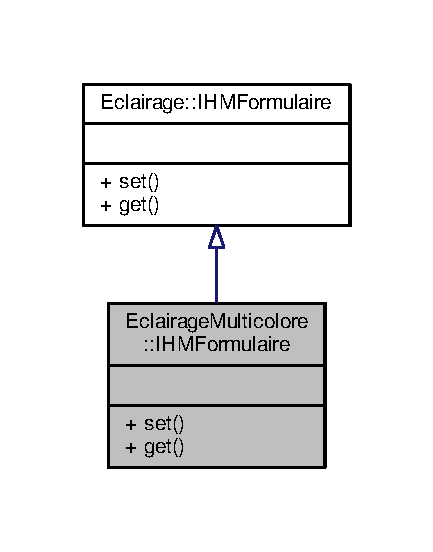
\includegraphics[width=208pt]{classEclairageMulticolore_1_1IHMFormulaire__inherit__graph}
\end{center}
\end{figure}


Graphe de collaboration de Eclairage\+Multicolore\+:\+:I\+H\+M\+Formulaire\+:
\nopagebreak
\begin{figure}[H]
\begin{center}
\leavevmode
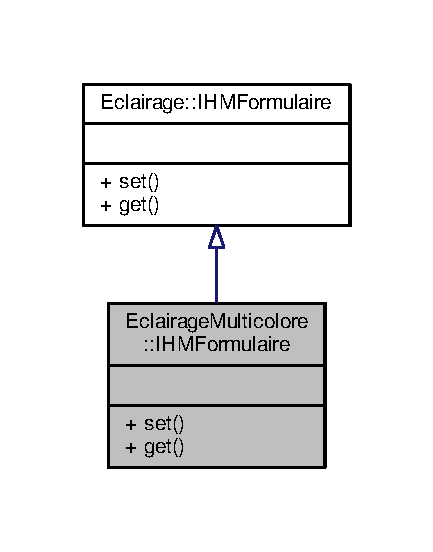
\includegraphics[width=208pt]{classEclairageMulticolore_1_1IHMFormulaire__coll__graph}
\end{center}
\end{figure}
\subsection*{Fonctions membres publiques}
\begin{DoxyCompactItemize}
\item 
void \hyperlink{classEclairageMulticolore_1_1IHMFormulaire_a80490fb7a2afb787d822a7bc53775979}{set} (\hyperlink{classEclairageMulticolore_1_1Ent}{Eclairage\+Multicolore\+::\+Ent} \&ent, std\+::string nom, std\+::string couleur, std\+::string id)
\item 
void \hyperlink{classEclairageMulticolore_1_1IHMFormulaire_a30d214645d58e1ba5439a4cb76f0b30c}{get} (\hyperlink{classEclairageMulticolore_1_1Ent}{Eclairage\+Multicolore\+::\+Ent} \&ent)
\end{DoxyCompactItemize}


\subsection{Description détaillée}
I\+HM pr�sentant au propri�taire un forulaire de cr�ation d\textquotesingle{}�clairage multicolore. 

\subsection{Documentation des fonctions membres}
\mbox{\Hypertarget{classEclairageMulticolore_1_1IHMFormulaire_a30d214645d58e1ba5439a4cb76f0b30c}\label{classEclairageMulticolore_1_1IHMFormulaire_a30d214645d58e1ba5439a4cb76f0b30c}} 
\index{Eclairage\+Multicolore\+::\+I\+H\+M\+Formulaire@{Eclairage\+Multicolore\+::\+I\+H\+M\+Formulaire}!get@{get}}
\index{get@{get}!Eclairage\+Multicolore\+::\+I\+H\+M\+Formulaire@{Eclairage\+Multicolore\+::\+I\+H\+M\+Formulaire}}
\subsubsection{\texorpdfstring{get()}{get()}}
{\footnotesize\ttfamily void Eclairage\+Multicolore\+::\+I\+H\+M\+Formulaire\+::get (\begin{DoxyParamCaption}\item[{\hyperlink{classEclairageMulticolore_1_1Ent}{Eclairage\+Multicolore\+::\+Ent} \&}]{ent }\end{DoxyParamCaption})}

M�thode permettant de r�cup�rer les donn�es entr�es par l\textquotesingle{}utilisateur lors de la cr�ation d\textquotesingle{}�clairage multicolore. \mbox{\Hypertarget{classEclairageMulticolore_1_1IHMFormulaire_a80490fb7a2afb787d822a7bc53775979}\label{classEclairageMulticolore_1_1IHMFormulaire_a80490fb7a2afb787d822a7bc53775979}} 
\index{Eclairage\+Multicolore\+::\+I\+H\+M\+Formulaire@{Eclairage\+Multicolore\+::\+I\+H\+M\+Formulaire}!set@{set}}
\index{set@{set}!Eclairage\+Multicolore\+::\+I\+H\+M\+Formulaire@{Eclairage\+Multicolore\+::\+I\+H\+M\+Formulaire}}
\subsubsection{\texorpdfstring{set()}{set()}}
{\footnotesize\ttfamily void Eclairage\+Multicolore\+::\+I\+H\+M\+Formulaire\+::set (\begin{DoxyParamCaption}\item[{\hyperlink{classEclairageMulticolore_1_1Ent}{Eclairage\+Multicolore\+::\+Ent} \&}]{ent,  }\item[{std\+::string}]{nom,  }\item[{std\+::string}]{couleur,  }\item[{std\+::string}]{id }\end{DoxyParamCaption})}

M�thde permettant d\textquotesingle{}afficher le formulaire de cr�ation d\textquotesingle{}�clairage multicolore 

Références Fichier\+Texte\+Persi\+Bny\+::get\+Contenu().



La documentation de cette classe a été générée à partir des fichiers suivants \+:\begin{DoxyCompactItemize}
\item 
src/\hyperlink{EclairageMulticolore_8h}{Eclairage\+Multicolore.\+h}\item 
src/\hyperlink{EclairageMulticolore_8cpp}{Eclairage\+Multicolore.\+cpp}\end{DoxyCompactItemize}

\hypertarget{classEclairageUnicolore_1_1IHMFormulaire}{}\section{Référence de la classe Eclairage\+Unicolore\+:\+:I\+H\+M\+Formulaire}
\label{classEclairageUnicolore_1_1IHMFormulaire}\index{Eclairage\+Unicolore\+::\+I\+H\+M\+Formulaire@{Eclairage\+Unicolore\+::\+I\+H\+M\+Formulaire}}


{\ttfamily \#include $<$Eclairage\+Unicolore.\+h$>$}



Graphe d\textquotesingle{}héritage de Eclairage\+Unicolore\+:\+:I\+H\+M\+Formulaire\+:
\nopagebreak
\begin{figure}[H]
\begin{center}
\leavevmode
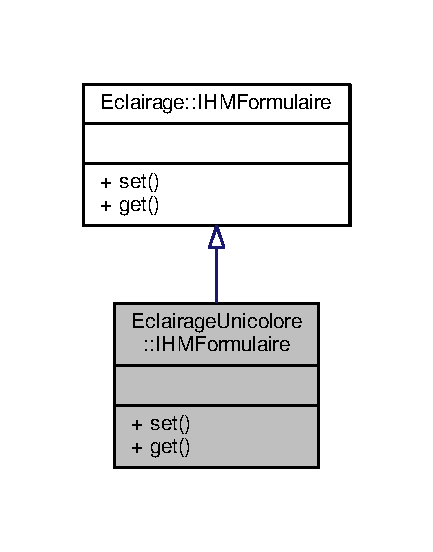
\includegraphics[width=208pt]{classEclairageUnicolore_1_1IHMFormulaire__inherit__graph}
\end{center}
\end{figure}


Graphe de collaboration de Eclairage\+Unicolore\+:\+:I\+H\+M\+Formulaire\+:
\nopagebreak
\begin{figure}[H]
\begin{center}
\leavevmode
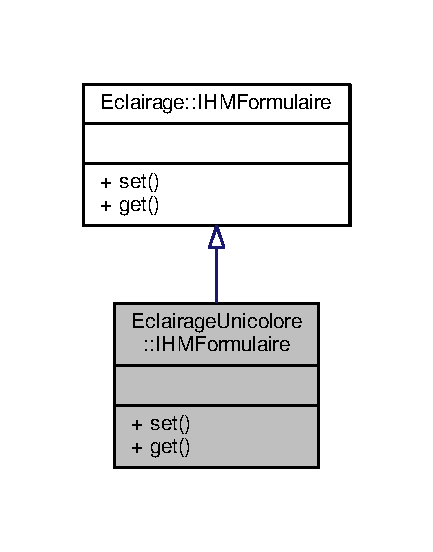
\includegraphics[width=208pt]{classEclairageUnicolore_1_1IHMFormulaire__coll__graph}
\end{center}
\end{figure}
\subsection*{Fonctions membres publiques}
\begin{DoxyCompactItemize}
\item 
void \hyperlink{classEclairageUnicolore_1_1IHMFormulaire_aea8ae2ab017bd6be151a563fe89fc267}{set} (\hyperlink{classEclairageUnicolore_1_1Ent}{Eclairage\+Unicolore\+::\+Ent} \&ent, std\+::string nom, std\+::string couleur, std\+::string id)
\item 
void \hyperlink{classEclairageUnicolore_1_1IHMFormulaire_a80c57e8124f32a53f6d5eee260e765c3}{get} (\hyperlink{classEclairageUnicolore_1_1Ent}{Eclairage\+Unicolore\+::\+Ent} \&ent)
\end{DoxyCompactItemize}


\subsection{Description détaillée}
I\+HM pr�sentant au propri�taire un forulaire de cr�ation d\textquotesingle{}�clairage unicolore. 

\subsection{Documentation des fonctions membres}
\mbox{\Hypertarget{classEclairageUnicolore_1_1IHMFormulaire_a80c57e8124f32a53f6d5eee260e765c3}\label{classEclairageUnicolore_1_1IHMFormulaire_a80c57e8124f32a53f6d5eee260e765c3}} 
\index{Eclairage\+Unicolore\+::\+I\+H\+M\+Formulaire@{Eclairage\+Unicolore\+::\+I\+H\+M\+Formulaire}!get@{get}}
\index{get@{get}!Eclairage\+Unicolore\+::\+I\+H\+M\+Formulaire@{Eclairage\+Unicolore\+::\+I\+H\+M\+Formulaire}}
\subsubsection{\texorpdfstring{get()}{get()}}
{\footnotesize\ttfamily void Eclairage\+Unicolore\+::\+I\+H\+M\+Formulaire\+::get (\begin{DoxyParamCaption}\item[{\hyperlink{classEclairageUnicolore_1_1Ent}{Eclairage\+Unicolore\+::\+Ent} \&}]{ent }\end{DoxyParamCaption})}

M�thode permettant de r�cup�rer les donn�es entr�es par l\textquotesingle{}utilisateur lors de la cr�ation d\textquotesingle{}�clairage unicolore. \mbox{\Hypertarget{classEclairageUnicolore_1_1IHMFormulaire_aea8ae2ab017bd6be151a563fe89fc267}\label{classEclairageUnicolore_1_1IHMFormulaire_aea8ae2ab017bd6be151a563fe89fc267}} 
\index{Eclairage\+Unicolore\+::\+I\+H\+M\+Formulaire@{Eclairage\+Unicolore\+::\+I\+H\+M\+Formulaire}!set@{set}}
\index{set@{set}!Eclairage\+Unicolore\+::\+I\+H\+M\+Formulaire@{Eclairage\+Unicolore\+::\+I\+H\+M\+Formulaire}}
\subsubsection{\texorpdfstring{set()}{set()}}
{\footnotesize\ttfamily void Eclairage\+Unicolore\+::\+I\+H\+M\+Formulaire\+::set (\begin{DoxyParamCaption}\item[{\hyperlink{classEclairageUnicolore_1_1Ent}{Eclairage\+Unicolore\+::\+Ent} \&}]{ent,  }\item[{std\+::string}]{nom,  }\item[{std\+::string}]{couleur,  }\item[{std\+::string}]{id }\end{DoxyParamCaption})}

M�thde permettant d\textquotesingle{}afficher le formulaire de cr�ation d\textquotesingle{}�clairage unicolore 

Références Fichier\+Texte\+Persi\+Bny\+::get\+Contenu().



La documentation de cette classe a été générée à partir des fichiers suivants \+:\begin{DoxyCompactItemize}
\item 
src/\hyperlink{EclairageUnicolore_8h}{Eclairage\+Unicolore.\+h}\item 
src/\hyperlink{EclairageUnicolore_8cpp}{Eclairage\+Unicolore.\+cpp}\end{DoxyCompactItemize}

\hypertarget{classEclairage_1_1IHMFormulaire}{}\section{Référence de la classe Eclairage\+:\+:I\+H\+M\+Formulaire}
\label{classEclairage_1_1IHMFormulaire}\index{Eclairage\+::\+I\+H\+M\+Formulaire@{Eclairage\+::\+I\+H\+M\+Formulaire}}


{\ttfamily \#include $<$Eclairage.\+h$>$}



Graphe d\textquotesingle{}héritage de Eclairage\+:\+:I\+H\+M\+Formulaire\+:
\nopagebreak
\begin{figure}[H]
\begin{center}
\leavevmode
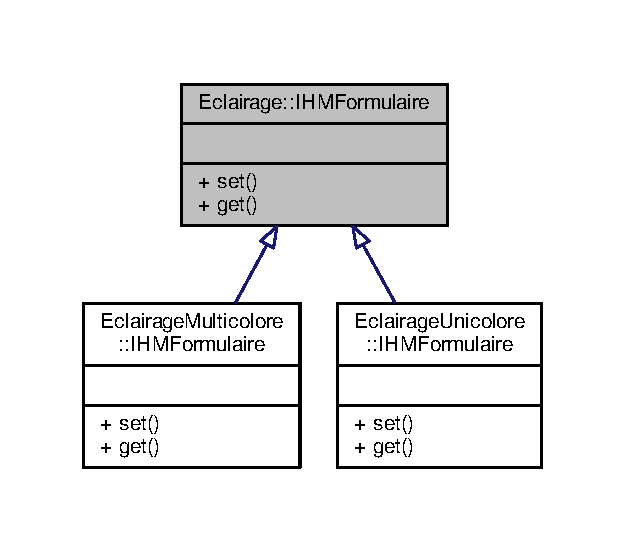
\includegraphics[width=300pt]{classEclairage_1_1IHMFormulaire__inherit__graph}
\end{center}
\end{figure}


Graphe de collaboration de Eclairage\+:\+:I\+H\+M\+Formulaire\+:
\nopagebreak
\begin{figure}[H]
\begin{center}
\leavevmode
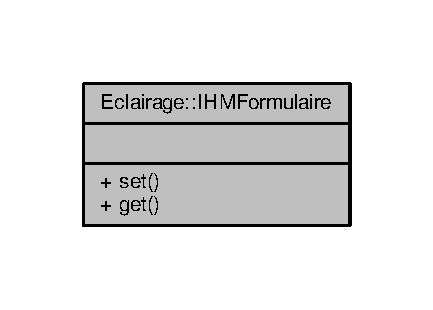
\includegraphics[width=208pt]{classEclairage_1_1IHMFormulaire__coll__graph}
\end{center}
\end{figure}
\subsection*{Fonctions membres publiques}
\begin{DoxyCompactItemize}
\item 
void \hyperlink{classEclairage_1_1IHMFormulaire_a182c4a46d4dc3ba1ad8e146715ffff94}{set} (\hyperlink{classEclairage_1_1Ent}{Eclairage\+::\+Ent} \&ent, std\+::string type)
\item 
void \hyperlink{classEclairage_1_1IHMFormulaire_a912c6c0ad0c844b0509fb9154753bfc9}{get} (\hyperlink{classEclairage_1_1Ent}{Eclairage\+::\+Ent} \&ent)
\end{DoxyCompactItemize}


\subsection{Description détaillée}
I\+HM pr�sentant au propri�taire un forulaire de cr�ation d\textquotesingle{}�clairage. 

\subsection{Documentation des fonctions membres}
\mbox{\Hypertarget{classEclairage_1_1IHMFormulaire_a912c6c0ad0c844b0509fb9154753bfc9}\label{classEclairage_1_1IHMFormulaire_a912c6c0ad0c844b0509fb9154753bfc9}} 
\index{Eclairage\+::\+I\+H\+M\+Formulaire@{Eclairage\+::\+I\+H\+M\+Formulaire}!get@{get}}
\index{get@{get}!Eclairage\+::\+I\+H\+M\+Formulaire@{Eclairage\+::\+I\+H\+M\+Formulaire}}
\subsubsection{\texorpdfstring{get()}{get()}}
{\footnotesize\ttfamily void Eclairage\+::\+I\+H\+M\+Formulaire\+::get (\begin{DoxyParamCaption}\item[{\hyperlink{classEclairage_1_1Ent}{Eclairage\+::\+Ent} \&}]{ent }\end{DoxyParamCaption})}

M�thode permettant de r�cup�rer les donn�es entr�es par l\textquotesingle{}utilisateur lors de la cr�ation d\textquotesingle{}�clairage. 

Références Blanc, Bleu, Rouge, Eclairage\+::\+Ent\+::set\+Couleur(), et Eclairage\+::\+Ent\+::set\+Nom().

\mbox{\Hypertarget{classEclairage_1_1IHMFormulaire_a182c4a46d4dc3ba1ad8e146715ffff94}\label{classEclairage_1_1IHMFormulaire_a182c4a46d4dc3ba1ad8e146715ffff94}} 
\index{Eclairage\+::\+I\+H\+M\+Formulaire@{Eclairage\+::\+I\+H\+M\+Formulaire}!set@{set}}
\index{set@{set}!Eclairage\+::\+I\+H\+M\+Formulaire@{Eclairage\+::\+I\+H\+M\+Formulaire}}
\subsubsection{\texorpdfstring{set()}{set()}}
{\footnotesize\ttfamily void Eclairage\+::\+I\+H\+M\+Formulaire\+::set (\begin{DoxyParamCaption}\item[{\hyperlink{classEclairage_1_1Ent}{Eclairage\+::\+Ent} \&}]{ent,  }\item[{std\+::string}]{type }\end{DoxyParamCaption})}

M�thde permettant d\textquotesingle{}afficher le formulaire de cr�ation d\textquotesingle{}�clairage 

Références Fichier\+Texte\+Persi\+Bny\+::get\+Contenu(), et Eclairage\+::\+Ent\+::get\+I\+D().



La documentation de cette classe a été générée à partir des fichiers suivants \+:\begin{DoxyCompactItemize}
\item 
src/\hyperlink{Eclairage_8h}{Eclairage.\+h}\item 
src/\hyperlink{Eclairage_8cpp}{Eclairage.\+cpp}\end{DoxyCompactItemize}

\hypertarget{classEclairage_1_1IHMJardin}{}\section{Référence de la classe Eclairage\+:\+:I\+H\+M\+Jardin}
\label{classEclairage_1_1IHMJardin}\index{Eclairage\+::\+I\+H\+M\+Jardin@{Eclairage\+::\+I\+H\+M\+Jardin}}


{\ttfamily \#include $<$Eclairage.\+h$>$}



Graphe d\textquotesingle{}héritage de Eclairage\+:\+:I\+H\+M\+Jardin\+:
\nopagebreak
\begin{figure}[H]
\begin{center}
\leavevmode
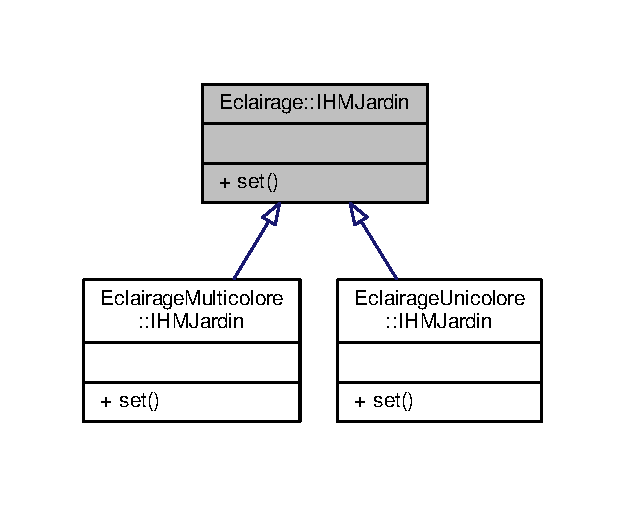
\includegraphics[width=300pt]{classEclairage_1_1IHMJardin__inherit__graph}
\end{center}
\end{figure}


Graphe de collaboration de Eclairage\+:\+:I\+H\+M\+Jardin\+:
\nopagebreak
\begin{figure}[H]
\begin{center}
\leavevmode
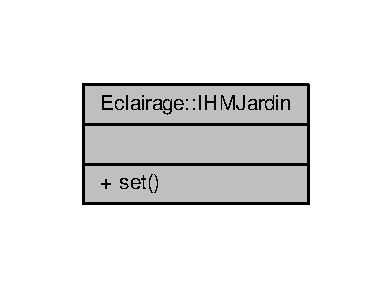
\includegraphics[width=188pt]{classEclairage_1_1IHMJardin__coll__graph}
\end{center}
\end{figure}
\subsection*{Fonctions membres publiques}
\begin{DoxyCompactItemize}
\item 
void \hyperlink{classEclairage_1_1IHMJardin_a2be27eea035e7973fc6f649be85f2a0b}{set} (const \hyperlink{classEclairage_1_1Ent}{Eclairage\+::\+Ent} \&ent)
\end{DoxyCompactItemize}


\subsection{Documentation des fonctions membres}
\mbox{\Hypertarget{classEclairage_1_1IHMJardin_a2be27eea035e7973fc6f649be85f2a0b}\label{classEclairage_1_1IHMJardin_a2be27eea035e7973fc6f649be85f2a0b}} 
\index{Eclairage\+::\+I\+H\+M\+Jardin@{Eclairage\+::\+I\+H\+M\+Jardin}!set@{set}}
\index{set@{set}!Eclairage\+::\+I\+H\+M\+Jardin@{Eclairage\+::\+I\+H\+M\+Jardin}}
\subsubsection{\texorpdfstring{set()}{set()}}
{\footnotesize\ttfamily void Eclairage\+::\+I\+H\+M\+Jardin\+::set (\begin{DoxyParamCaption}\item[{const \hyperlink{classEclairage_1_1Ent}{Eclairage\+::\+Ent} \&}]{ent }\end{DoxyParamCaption})}

M�thode permettant de mettre � jour l\textquotesingle{}icone repr�sentant l\textquotesingle{}�clairage dans l\textquotesingle{}I\+HM de supervision. 

Références Eclairage\+::controleur, Eclairage\+::\+Controleur\+::ent, Eclairage\+::\+Controleur\+::persi\+Bny, et Eclairage\+::\+Persi\+Bny\+::set().



La documentation de cette classe a été générée à partir des fichiers suivants \+:\begin{DoxyCompactItemize}
\item 
src/\hyperlink{Eclairage_8h}{Eclairage.\+h}\item 
src/\hyperlink{Eclairage_8cpp}{Eclairage.\+cpp}\end{DoxyCompactItemize}

\hypertarget{classEclairageUnicolore_1_1IHMJardin}{}\section{Référence de la classe Eclairage\+Unicolore\+:\+:I\+H\+M\+Jardin}
\label{classEclairageUnicolore_1_1IHMJardin}\index{Eclairage\+Unicolore\+::\+I\+H\+M\+Jardin@{Eclairage\+Unicolore\+::\+I\+H\+M\+Jardin}}


{\ttfamily \#include $<$Eclairage\+Unicolore.\+h$>$}



Graphe d\textquotesingle{}héritage de Eclairage\+Unicolore\+:\+:I\+H\+M\+Jardin\+:
\nopagebreak
\begin{figure}[H]
\begin{center}
\leavevmode
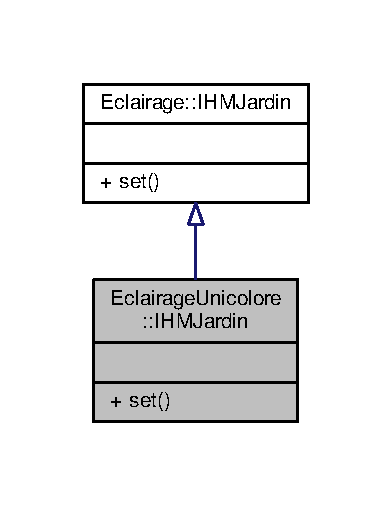
\includegraphics[width=188pt]{classEclairageUnicolore_1_1IHMJardin__inherit__graph}
\end{center}
\end{figure}


Graphe de collaboration de Eclairage\+Unicolore\+:\+:I\+H\+M\+Jardin\+:
\nopagebreak
\begin{figure}[H]
\begin{center}
\leavevmode
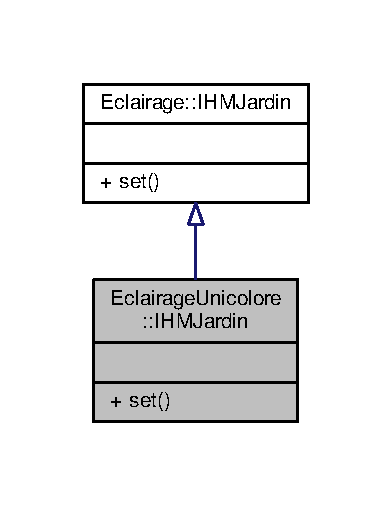
\includegraphics[width=188pt]{classEclairageUnicolore_1_1IHMJardin__coll__graph}
\end{center}
\end{figure}
\subsection*{Fonctions membres publiques}
\begin{DoxyCompactItemize}
\item 
void \hyperlink{classEclairageUnicolore_1_1IHMJardin_ad96a0bac27e2ce81a8d4403a296b78f3}{set} (\hyperlink{classEclairageUnicolore_1_1Ent}{Eclairage\+Unicolore\+::\+Ent} \&ent)
\end{DoxyCompactItemize}


\subsection{Description détaillée}
Classe permettant d\textquotesingle{}afficher l\textquotesingle{}I\+HM de l\textquotesingle{}�clairage dans le jardin 

\subsection{Documentation des fonctions membres}
\mbox{\Hypertarget{classEclairageUnicolore_1_1IHMJardin_ad96a0bac27e2ce81a8d4403a296b78f3}\label{classEclairageUnicolore_1_1IHMJardin_ad96a0bac27e2ce81a8d4403a296b78f3}} 
\index{Eclairage\+Unicolore\+::\+I\+H\+M\+Jardin@{Eclairage\+Unicolore\+::\+I\+H\+M\+Jardin}!set@{set}}
\index{set@{set}!Eclairage\+Unicolore\+::\+I\+H\+M\+Jardin@{Eclairage\+Unicolore\+::\+I\+H\+M\+Jardin}}
\subsubsection{\texorpdfstring{set()}{set()}}
{\footnotesize\ttfamily void Eclairage\+Unicolore\+::\+I\+H\+M\+Jardin\+::set (\begin{DoxyParamCaption}\item[{\hyperlink{classEclairageUnicolore_1_1Ent}{Eclairage\+Unicolore\+::\+Ent} \&}]{ent }\end{DoxyParamCaption})}

M�thode permettant de mettre � jour l\textquotesingle{}icone repr�sentant l\textquotesingle{}�clairage dans l\textquotesingle{}I\+HM de supervision. 

Références Eclairage\+::\+Ent\+::get\+Active(), Eclairage\+::\+Ent\+::get\+Allume(), Eclairage\+::\+Ent\+::get\+Couleur(), Eclairage\+::\+Ent\+::get\+I\+D(), Eclairage\+::\+Ent\+::get\+X(), et Eclairage\+::\+Ent\+::get\+Y().



La documentation de cette classe a été générée à partir des fichiers suivants \+:\begin{DoxyCompactItemize}
\item 
src/\hyperlink{EclairageUnicolore_8h}{Eclairage\+Unicolore.\+h}\item 
src/\hyperlink{EclairageUnicolore_8cpp}{Eclairage\+Unicolore.\+cpp}\end{DoxyCompactItemize}

\hypertarget{classEclairageMulticolore_1_1IHMJardin}{}\section{Référence de la classe Eclairage\+Multicolore\+:\+:I\+H\+M\+Jardin}
\label{classEclairageMulticolore_1_1IHMJardin}\index{Eclairage\+Multicolore\+::\+I\+H\+M\+Jardin@{Eclairage\+Multicolore\+::\+I\+H\+M\+Jardin}}


{\ttfamily \#include $<$Eclairage\+Multicolore.\+h$>$}



Graphe d\textquotesingle{}héritage de Eclairage\+Multicolore\+:\+:I\+H\+M\+Jardin\+:
\nopagebreak
\begin{figure}[H]
\begin{center}
\leavevmode
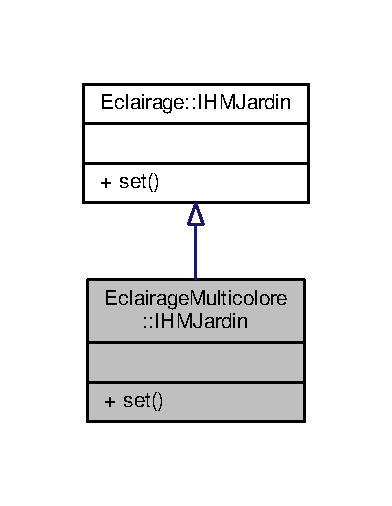
\includegraphics[width=188pt]{classEclairageMulticolore_1_1IHMJardin__inherit__graph}
\end{center}
\end{figure}


Graphe de collaboration de Eclairage\+Multicolore\+:\+:I\+H\+M\+Jardin\+:
\nopagebreak
\begin{figure}[H]
\begin{center}
\leavevmode
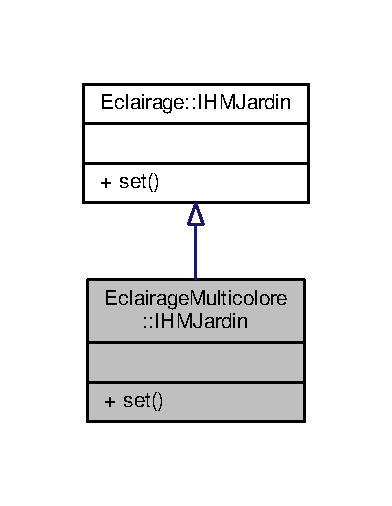
\includegraphics[width=188pt]{classEclairageMulticolore_1_1IHMJardin__coll__graph}
\end{center}
\end{figure}
\subsection*{Fonctions membres publiques}
\begin{DoxyCompactItemize}
\item 
void \hyperlink{classEclairageMulticolore_1_1IHMJardin_a9caf35735546e5d36e72ce509da5b14c}{set} (\hyperlink{classEclairageMulticolore_1_1Ent}{Eclairage\+Multicolore\+::\+Ent} \&ent)
\end{DoxyCompactItemize}


\subsection{Documentation des fonctions membres}
\mbox{\Hypertarget{classEclairageMulticolore_1_1IHMJardin_a9caf35735546e5d36e72ce509da5b14c}\label{classEclairageMulticolore_1_1IHMJardin_a9caf35735546e5d36e72ce509da5b14c}} 
\index{Eclairage\+Multicolore\+::\+I\+H\+M\+Jardin@{Eclairage\+Multicolore\+::\+I\+H\+M\+Jardin}!set@{set}}
\index{set@{set}!Eclairage\+Multicolore\+::\+I\+H\+M\+Jardin@{Eclairage\+Multicolore\+::\+I\+H\+M\+Jardin}}
\subsubsection{\texorpdfstring{set()}{set()}}
{\footnotesize\ttfamily void Eclairage\+Multicolore\+::\+I\+H\+M\+Jardin\+::set (\begin{DoxyParamCaption}\item[{\hyperlink{classEclairageMulticolore_1_1Ent}{Eclairage\+Multicolore\+::\+Ent} \&}]{ent }\end{DoxyParamCaption})}

M�thode permettant de mettre � jour l\textquotesingle{}icone repr�sentant l\textquotesingle{}�clairage dans l\textquotesingle{}I\+HM de supervision. 

Références Eclairage\+::\+Ent\+::get\+Active(), Eclairage\+::\+Ent\+::get\+Allume(), Eclairage\+::\+Ent\+::get\+Couleur(), et Eclairage\+::\+Ent\+::get\+I\+D().



La documentation de cette classe a été générée à partir des fichiers suivants \+:\begin{DoxyCompactItemize}
\item 
src/\hyperlink{EclairageMulticolore_8h}{Eclairage\+Multicolore.\+h}\item 
src/\hyperlink{EclairageMulticolore_8cpp}{Eclairage\+Multicolore.\+cpp}\end{DoxyCompactItemize}

\hypertarget{classEclairageMulticolore_1_1IHMParametre}{}\section{Référence de la classe Eclairage\+Multicolore\+:\+:I\+H\+M\+Parametre}
\label{classEclairageMulticolore_1_1IHMParametre}\index{Eclairage\+Multicolore\+::\+I\+H\+M\+Parametre@{Eclairage\+Multicolore\+::\+I\+H\+M\+Parametre}}


{\ttfamily \#include $<$Eclairage\+Multicolore.\+h$>$}



Graphe de collaboration de Eclairage\+Multicolore\+:\+:I\+H\+M\+Parametre\+:
\nopagebreak
\begin{figure}[H]
\begin{center}
\leavevmode
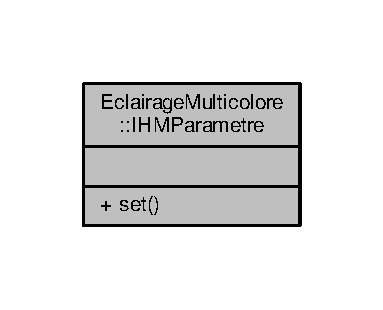
\includegraphics[width=184pt]{classEclairageMulticolore_1_1IHMParametre__coll__graph}
\end{center}
\end{figure}
\subsection*{Fonctions membres publiques}
\begin{DoxyCompactItemize}
\item 
void \hyperlink{classEclairageMulticolore_1_1IHMParametre_a2ed609d0e667d937d8e4b686b93af18c}{set} (\hyperlink{classEclairageMulticolore_1_1Ent}{Eclairage\+Multicolore\+::\+Ent} \&ent)
\end{DoxyCompactItemize}


\subsection{Documentation des fonctions membres}
\mbox{\Hypertarget{classEclairageMulticolore_1_1IHMParametre_a2ed609d0e667d937d8e4b686b93af18c}\label{classEclairageMulticolore_1_1IHMParametre_a2ed609d0e667d937d8e4b686b93af18c}} 
\index{Eclairage\+Multicolore\+::\+I\+H\+M\+Parametre@{Eclairage\+Multicolore\+::\+I\+H\+M\+Parametre}!set@{set}}
\index{set@{set}!Eclairage\+Multicolore\+::\+I\+H\+M\+Parametre@{Eclairage\+Multicolore\+::\+I\+H\+M\+Parametre}}
\subsubsection{\texorpdfstring{set()}{set()}}
{\footnotesize\ttfamily void Eclairage\+Multicolore\+::\+I\+H\+M\+Parametre\+::set (\begin{DoxyParamCaption}\item[{\hyperlink{classEclairageMulticolore_1_1Ent}{Eclairage\+Multicolore\+::\+Ent} \&}]{ent }\end{DoxyParamCaption})}



Références Sqlite\+Persi\+Bny\+::executer\+Sql(), Fichier\+Texte\+Persi\+Bny\+::get\+Contenu(), et Eclairage\+::\+Ent\+::get\+I\+D().



La documentation de cette classe a été générée à partir des fichiers suivants \+:\begin{DoxyCompactItemize}
\item 
src/\hyperlink{EclairageMulticolore_8h}{Eclairage\+Multicolore.\+h}\item 
src/\hyperlink{EclairageMulticolore_8cpp}{Eclairage\+Multicolore.\+cpp}\end{DoxyCompactItemize}

\hypertarget{classEclairageUnicolore_1_1IHMParametre}{}\section{Référence de la classe Eclairage\+Unicolore\+:\+:I\+H\+M\+Parametre}
\label{classEclairageUnicolore_1_1IHMParametre}\index{Eclairage\+Unicolore\+::\+I\+H\+M\+Parametre@{Eclairage\+Unicolore\+::\+I\+H\+M\+Parametre}}


{\ttfamily \#include $<$Eclairage\+Unicolore.\+h$>$}



Graphe de collaboration de Eclairage\+Unicolore\+:\+:I\+H\+M\+Parametre\+:
\nopagebreak
\begin{figure}[H]
\begin{center}
\leavevmode
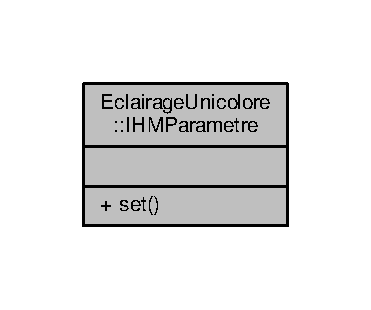
\includegraphics[width=178pt]{classEclairageUnicolore_1_1IHMParametre__coll__graph}
\end{center}
\end{figure}
\subsection*{Fonctions membres publiques}
\begin{DoxyCompactItemize}
\item 
void \hyperlink{classEclairageUnicolore_1_1IHMParametre_a2cdd87935914fc4f101fa63daf4af0d5}{set} (\hyperlink{classEclairageUnicolore_1_1Ent}{Eclairage\+Unicolore\+::\+Ent} \&ent)
\end{DoxyCompactItemize}


\subsection{Documentation des fonctions membres}
\mbox{\Hypertarget{classEclairageUnicolore_1_1IHMParametre_a2cdd87935914fc4f101fa63daf4af0d5}\label{classEclairageUnicolore_1_1IHMParametre_a2cdd87935914fc4f101fa63daf4af0d5}} 
\index{Eclairage\+Unicolore\+::\+I\+H\+M\+Parametre@{Eclairage\+Unicolore\+::\+I\+H\+M\+Parametre}!set@{set}}
\index{set@{set}!Eclairage\+Unicolore\+::\+I\+H\+M\+Parametre@{Eclairage\+Unicolore\+::\+I\+H\+M\+Parametre}}
\subsubsection{\texorpdfstring{set()}{set()}}
{\footnotesize\ttfamily void Eclairage\+Unicolore\+::\+I\+H\+M\+Parametre\+::set (\begin{DoxyParamCaption}\item[{\hyperlink{classEclairageUnicolore_1_1Ent}{Eclairage\+Unicolore\+::\+Ent} \&}]{ent }\end{DoxyParamCaption})}



Références Sqlite\+Persi\+Bny\+::executer\+Sql(), Fichier\+Texte\+Persi\+Bny\+::get\+Contenu(), et Eclairage\+::\+Ent\+::get\+I\+D().



La documentation de cette classe a été générée à partir des fichiers suivants \+:\begin{DoxyCompactItemize}
\item 
src/\hyperlink{EclairageUnicolore_8h}{Eclairage\+Unicolore.\+h}\item 
src/\hyperlink{EclairageUnicolore_8cpp}{Eclairage\+Unicolore.\+cpp}\end{DoxyCompactItemize}

\hypertarget{classEclairageMulticolore_1_1PersiBny}{}\section{Référence de la classe Eclairage\+Multicolore\+:\+:Persi\+Bny}
\label{classEclairageMulticolore_1_1PersiBny}\index{Eclairage\+Multicolore\+::\+Persi\+Bny@{Eclairage\+Multicolore\+::\+Persi\+Bny}}


{\ttfamily \#include $<$Eclairage\+Multicolore.\+h$>$}



Graphe d\textquotesingle{}héritage de Eclairage\+Multicolore\+:\+:Persi\+Bny\+:\nopagebreak
\begin{figure}[H]
\begin{center}
\leavevmode
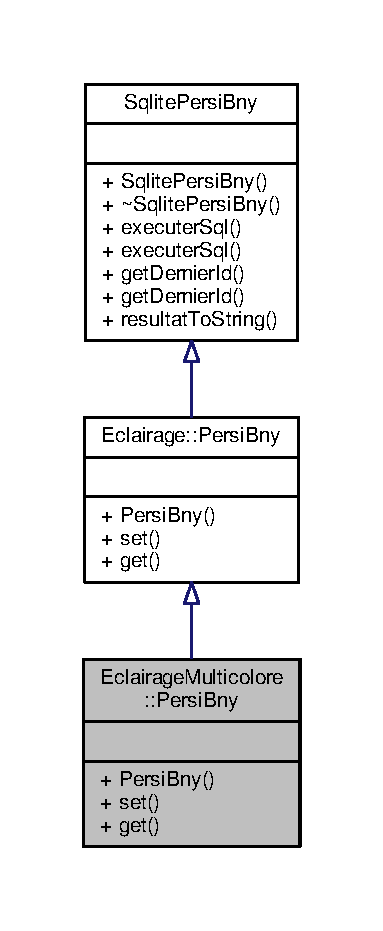
\includegraphics[width=184pt]{classEclairageMulticolore_1_1PersiBny__inherit__graph}
\end{center}
\end{figure}


Graphe de collaboration de Eclairage\+Multicolore\+:\+:Persi\+Bny\+:\nopagebreak
\begin{figure}[H]
\begin{center}
\leavevmode
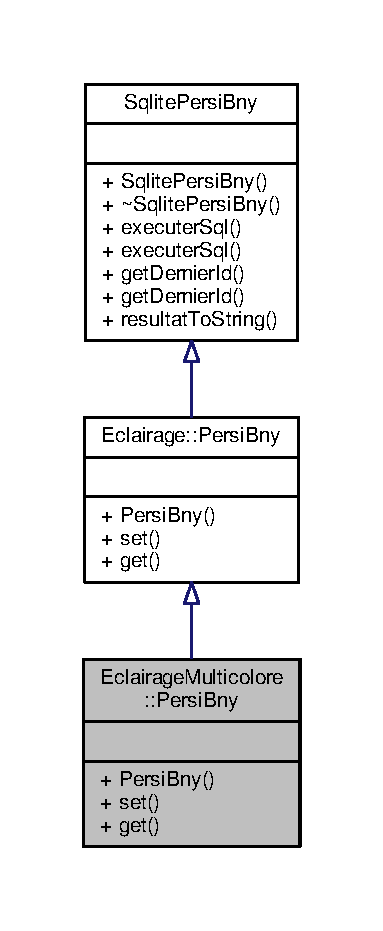
\includegraphics[width=184pt]{classEclairageMulticolore_1_1PersiBny__coll__graph}
\end{center}
\end{figure}
\subsection*{Membres hérités additionnels}


La documentation de cette classe a été générée à partir du fichier suivant \+:\begin{DoxyCompactItemize}
\item 
src/\hyperlink{EclairageMulticolore_8h}{Eclairage\+Multicolore.\+h}\end{DoxyCompactItemize}

\hypertarget{classEclairage_1_1PersiBny}{}\section{Référence de la classe Eclairage\+:\+:Persi\+Bny}
\label{classEclairage_1_1PersiBny}\index{Eclairage\+::\+Persi\+Bny@{Eclairage\+::\+Persi\+Bny}}


{\ttfamily \#include $<$Eclairage.\+h$>$}



Graphe d\textquotesingle{}héritage de Eclairage\+:\+:Persi\+Bny\+:
\nopagebreak
\begin{figure}[H]
\begin{center}
\leavevmode
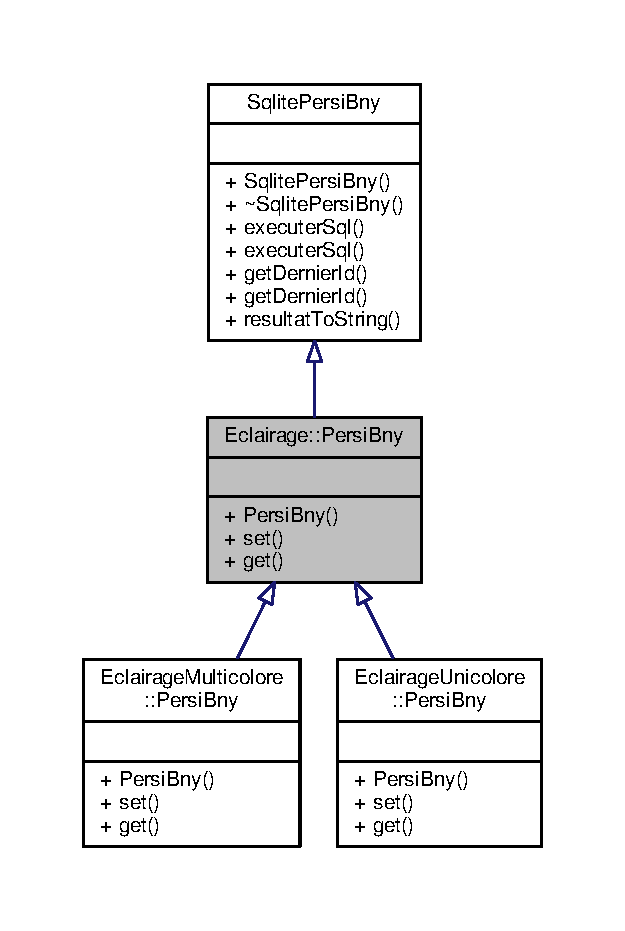
\includegraphics[width=300pt]{classEclairage_1_1PersiBny__inherit__graph}
\end{center}
\end{figure}


Graphe de collaboration de Eclairage\+:\+:Persi\+Bny\+:
\nopagebreak
\begin{figure}[H]
\begin{center}
\leavevmode
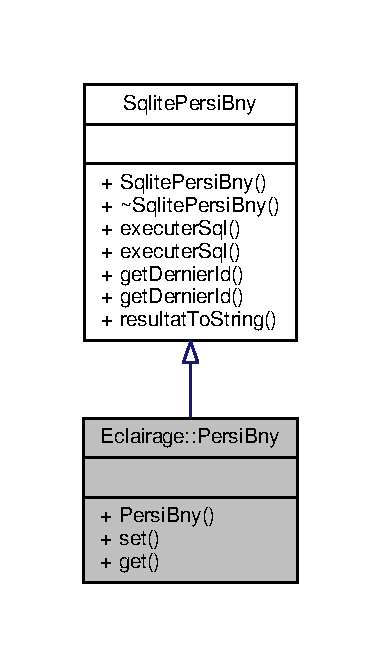
\includegraphics[width=183pt]{classEclairage_1_1PersiBny__coll__graph}
\end{center}
\end{figure}
\subsection*{Fonctions membres publiques}
\begin{DoxyCompactItemize}
\item 
\hyperlink{classEclairage_1_1PersiBny_abfb7c27bf74ca9a1e7e69d095df1be32}{Persi\+Bny} ()
\item 
void \hyperlink{classEclairage_1_1PersiBny_adf45a775e52135485a2cf5d6c7be9ecf}{set} (\hyperlink{classEclairage_1_1Ent}{Ent} \&ent)
\item 
void \hyperlink{classEclairage_1_1PersiBny_a77750fea340f129e56bde58be3984b56}{get} (\hyperlink{classEclairage_1_1Ent}{Ent} \&ent)
\end{DoxyCompactItemize}
\subsection*{Membres hérités additionnels}


\subsection{Documentation des constructeurs et destructeur}
\mbox{\Hypertarget{classEclairage_1_1PersiBny_abfb7c27bf74ca9a1e7e69d095df1be32}\label{classEclairage_1_1PersiBny_abfb7c27bf74ca9a1e7e69d095df1be32}} 
\index{Eclairage\+::\+Persi\+Bny@{Eclairage\+::\+Persi\+Bny}!Persi\+Bny@{Persi\+Bny}}
\index{Persi\+Bny@{Persi\+Bny}!Eclairage\+::\+Persi\+Bny@{Eclairage\+::\+Persi\+Bny}}
\subsubsection{\texorpdfstring{Persi\+Bny()}{PersiBny()}}
{\footnotesize\ttfamily Eclairage\+::\+Persi\+Bny\+::\+Persi\+Bny (\begin{DoxyParamCaption}{ }\end{DoxyParamCaption})\hspace{0.3cm}{\ttfamily [inline]}}

Constructeur de la persistance lui indiquant le fichier de base de donn�e. 

\subsection{Documentation des fonctions membres}
\mbox{\Hypertarget{classEclairage_1_1PersiBny_a77750fea340f129e56bde58be3984b56}\label{classEclairage_1_1PersiBny_a77750fea340f129e56bde58be3984b56}} 
\index{Eclairage\+::\+Persi\+Bny@{Eclairage\+::\+Persi\+Bny}!get@{get}}
\index{get@{get}!Eclairage\+::\+Persi\+Bny@{Eclairage\+::\+Persi\+Bny}}
\subsubsection{\texorpdfstring{get()}{get()}}
{\footnotesize\ttfamily void Eclairage\+::\+Persi\+Bny\+::get (\begin{DoxyParamCaption}\item[{\hyperlink{classEclairage_1_1Ent}{Ent} \&}]{ent }\end{DoxyParamCaption})}

M�thode permettant de r�cup�rer l\textquotesingle{}entit� de l\textquotesingle{}�clairage depuis la persistance. 

Références Blanc, Bleu, Eclairage\+::\+Ent\+::get\+I\+D(), Rouge, Eclairage\+::\+Ent\+::set\+Active(), Eclairage\+::\+Ent\+::set\+Allume(), Eclairage\+::\+Ent\+::set\+Consommation(), Eclairage\+::\+Ent\+::set\+Couleur(), Eclairage\+::\+Ent\+::set\+Nom(), Eclairage\+::\+Ent\+::set\+X(), et Eclairage\+::\+Ent\+::set\+Y().

\mbox{\Hypertarget{classEclairage_1_1PersiBny_adf45a775e52135485a2cf5d6c7be9ecf}\label{classEclairage_1_1PersiBny_adf45a775e52135485a2cf5d6c7be9ecf}} 
\index{Eclairage\+::\+Persi\+Bny@{Eclairage\+::\+Persi\+Bny}!set@{set}}
\index{set@{set}!Eclairage\+::\+Persi\+Bny@{Eclairage\+::\+Persi\+Bny}}
\subsubsection{\texorpdfstring{set()}{set()}}
{\footnotesize\ttfamily void Eclairage\+::\+Persi\+Bny\+::set (\begin{DoxyParamCaption}\item[{\hyperlink{classEclairage_1_1Ent}{Ent} \&}]{ent }\end{DoxyParamCaption})}

M�thode permettant de modifier la configuration de l\textquotesingle{}�clairage dans la persistance. 

Références Eclairage\+::\+Ent\+::get\+Active(), Eclairage\+::\+Ent\+::get\+Allume(), Eclairage\+::\+Ent\+::get\+Consommation(), Eclairage\+::\+Ent\+::get\+I\+D(), et Eclairage\+::\+Ent\+::get\+Nom().



La documentation de cette classe a été générée à partir des fichiers suivants \+:\begin{DoxyCompactItemize}
\item 
src/\hyperlink{Eclairage_8h}{Eclairage.\+h}\item 
src/\hyperlink{Eclairage_8cpp}{Eclairage.\+cpp}\end{DoxyCompactItemize}

\hypertarget{classEclairageUnicolore_1_1PersiBny}{}\section{Référence de la classe Eclairage\+Unicolore\+:\+:Persi\+Bny}
\label{classEclairageUnicolore_1_1PersiBny}\index{Eclairage\+Unicolore\+::\+Persi\+Bny@{Eclairage\+Unicolore\+::\+Persi\+Bny}}


{\ttfamily \#include $<$Eclairage\+Unicolore.\+h$>$}



Graphe d\textquotesingle{}héritage de Eclairage\+Unicolore\+:\+:Persi\+Bny\+:
\nopagebreak
\begin{figure}[H]
\begin{center}
\leavevmode
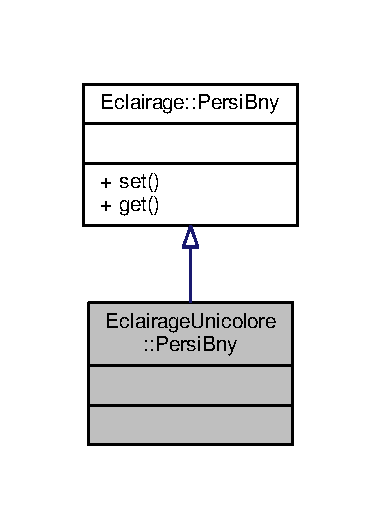
\includegraphics[width=183pt]{classEclairageUnicolore_1_1PersiBny__inherit__graph}
\end{center}
\end{figure}


Graphe de collaboration de Eclairage\+Unicolore\+:\+:Persi\+Bny\+:
\nopagebreak
\begin{figure}[H]
\begin{center}
\leavevmode
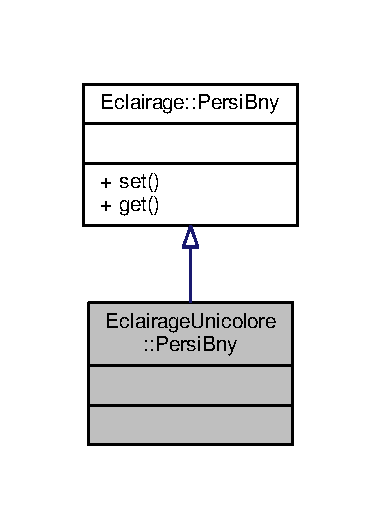
\includegraphics[width=183pt]{classEclairageUnicolore_1_1PersiBny__coll__graph}
\end{center}
\end{figure}
\subsection*{Fonctions membres publiques}
\begin{DoxyCompactItemize}
\item 
\hyperlink{classEclairageUnicolore_1_1PersiBny_aa039896a328787d64ad828ca3af0242a}{Persi\+Bny} ()
\item 
void \hyperlink{classEclairageUnicolore_1_1PersiBny_aaa52fce1a316dc779d3289ee1ac4c179}{set} (\hyperlink{classEclairageUnicolore_1_1Ent}{Ent} \&ent)
\item 
void \hyperlink{classEclairageUnicolore_1_1PersiBny_a7c6ed3b193f1b465bd0ac4d4dd6e6d52}{get} (\hyperlink{classEclairageUnicolore_1_1Ent}{Ent} \&ent)
\end{DoxyCompactItemize}
\subsection*{Membres hérités additionnels}


\subsection{Description détaillée}
Classe de persistance de l\textquotesingle{}�clairage d�rivant de la classe m�re \hyperlink{classEclairage_1_1PersiBny}{Eclairage\+::\+Persi\+Bny}. Permet de set et de get la configuration de l\textquotesingle{}�clairage dans la base de donn�es. 

\subsection{Documentation des constructeurs et destructeur}
\mbox{\Hypertarget{classEclairageUnicolore_1_1PersiBny_aa039896a328787d64ad828ca3af0242a}\label{classEclairageUnicolore_1_1PersiBny_aa039896a328787d64ad828ca3af0242a}} 
\index{Eclairage\+Unicolore\+::\+Persi\+Bny@{Eclairage\+Unicolore\+::\+Persi\+Bny}!Persi\+Bny@{Persi\+Bny}}
\index{Persi\+Bny@{Persi\+Bny}!Eclairage\+Unicolore\+::\+Persi\+Bny@{Eclairage\+Unicolore\+::\+Persi\+Bny}}
\subsubsection{\texorpdfstring{Persi\+Bny()}{PersiBny()}}
{\footnotesize\ttfamily Eclairage\+Unicolore\+::\+Persi\+Bny\+::\+Persi\+Bny (\begin{DoxyParamCaption}{ }\end{DoxyParamCaption})\hspace{0.3cm}{\ttfamily [inline]}}



\subsection{Documentation des fonctions membres}
\mbox{\Hypertarget{classEclairageUnicolore_1_1PersiBny_a7c6ed3b193f1b465bd0ac4d4dd6e6d52}\label{classEclairageUnicolore_1_1PersiBny_a7c6ed3b193f1b465bd0ac4d4dd6e6d52}} 
\index{Eclairage\+Unicolore\+::\+Persi\+Bny@{Eclairage\+Unicolore\+::\+Persi\+Bny}!get@{get}}
\index{get@{get}!Eclairage\+Unicolore\+::\+Persi\+Bny@{Eclairage\+Unicolore\+::\+Persi\+Bny}}
\subsubsection{\texorpdfstring{get()}{get()}}
{\footnotesize\ttfamily void Eclairage\+Unicolore\+::\+Persi\+Bny\+::get (\begin{DoxyParamCaption}\item[{\hyperlink{classEclairageUnicolore_1_1Ent}{Ent} \&}]{ent }\end{DoxyParamCaption})}

M�thode permettant de get la configuration de l\textquotesingle{}�clairage dans la base de donn�es. 

Références Eclairage\+Unicolore\+::controleur, Eclairage\+Unicolore\+::\+Controleur\+::ent, Eclairage\+::\+Persi\+Bny\+::get(), Eclairage\+::\+Ent\+::get\+I\+D(), Eclairage\+Unicolore\+::\+Controleur\+::ihm\+Formulaire, Rouge, Eclairage\+Unicolore\+::\+I\+H\+M\+Formulaire\+::set(), Eclairage\+::\+Ent\+::set\+Couleur(), Eclairage\+::\+Ent\+::set\+I\+D(), et Eclairage\+Unicolore\+::\+Ent\+::set\+Numero\+Prise().

\mbox{\Hypertarget{classEclairageUnicolore_1_1PersiBny_aaa52fce1a316dc779d3289ee1ac4c179}\label{classEclairageUnicolore_1_1PersiBny_aaa52fce1a316dc779d3289ee1ac4c179}} 
\index{Eclairage\+Unicolore\+::\+Persi\+Bny@{Eclairage\+Unicolore\+::\+Persi\+Bny}!set@{set}}
\index{set@{set}!Eclairage\+Unicolore\+::\+Persi\+Bny@{Eclairage\+Unicolore\+::\+Persi\+Bny}}
\subsubsection{\texorpdfstring{set()}{set()}}
{\footnotesize\ttfamily void Eclairage\+Unicolore\+::\+Persi\+Bny\+::set (\begin{DoxyParamCaption}\item[{\hyperlink{classEclairageUnicolore_1_1Ent}{Ent} \&}]{ent }\end{DoxyParamCaption})}

M�thode permettant de set la configuration de l\textquotesingle{}�clairage dans la base de donn�es. 

Références Eclairage\+::\+Ent\+::get\+Couleur(), Eclairage\+::\+Ent\+::get\+I\+D(), Eclairage\+Unicolore\+::\+Ent\+::get\+Numero\+Prise(), et Eclairage\+::\+Persi\+Bny\+::set().



La documentation de cette classe a été générée à partir des fichiers suivants \+:\begin{DoxyCompactItemize}
\item 
src/\hyperlink{EclairageUnicolore_8h}{Eclairage\+Unicolore.\+h}\item 
src/\hyperlink{EclairageUnicolore_8cpp}{Eclairage\+Unicolore.\+cpp}\end{DoxyCompactItemize}

\hypertarget{classSqlitePersiBny}{}\section{Référence de la classe Sqlite\+Persi\+Bny}
\label{classSqlitePersiBny}\index{Sqlite\+Persi\+Bny@{Sqlite\+Persi\+Bny}}


{\ttfamily \#include $<$Sqlite\+Persi\+Bny.\+h$>$}



Graphe d\textquotesingle{}héritage de Sqlite\+Persi\+Bny\+:
\nopagebreak
\begin{figure}[H]
\begin{center}
\leavevmode
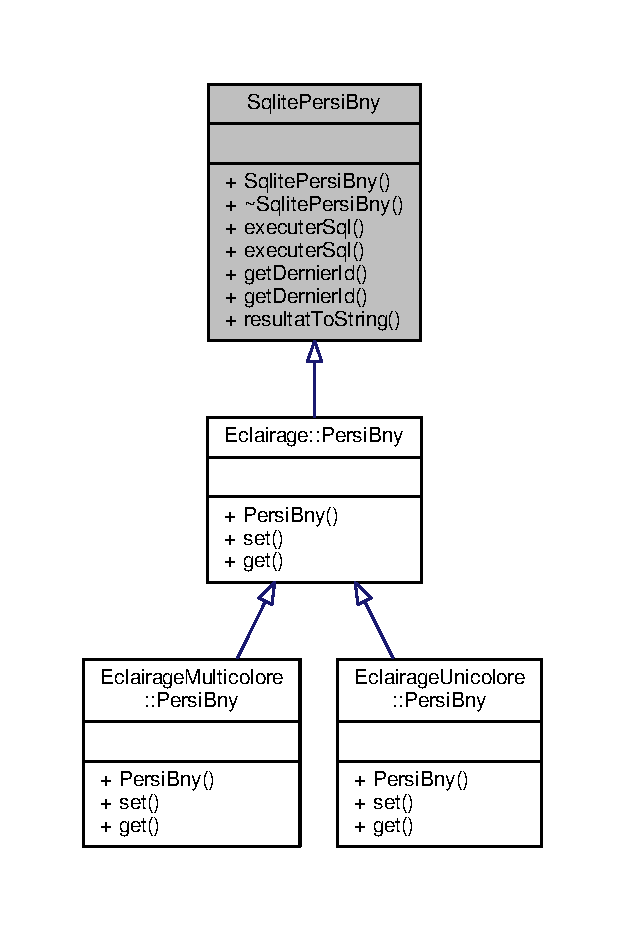
\includegraphics[width=300pt]{classSqlitePersiBny__inherit__graph}
\end{center}
\end{figure}


Graphe de collaboration de Sqlite\+Persi\+Bny\+:
\nopagebreak
\begin{figure}[H]
\begin{center}
\leavevmode
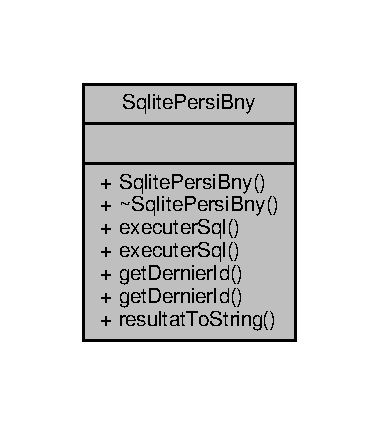
\includegraphics[width=182pt]{classSqlitePersiBny__coll__graph}
\end{center}
\end{figure}
\subsection*{Types publics}
\begin{DoxyCompactItemize}
\item 
typedef std\+::pair$<$ std\+::string, std\+::string $>$ \hyperlink{classSqlitePersiBny_af3de7ea7bd4146b4ce0a00ceae01befd}{Champs}
\item 
typedef std\+::vector$<$ \hyperlink{classSqlitePersiBny_af3de7ea7bd4146b4ce0a00ceae01befd}{Champs} $>$ \hyperlink{classSqlitePersiBny_a32400b54d9a08cae7d60d985a5d48892}{Ligne}
\item 
typedef std\+::vector$<$ \hyperlink{classSqlitePersiBny_a32400b54d9a08cae7d60d985a5d48892}{Ligne} $>$ \hyperlink{classSqlitePersiBny_a04bdd1bacd9241210ea44ec2c072f79b}{Resultat}
\end{DoxyCompactItemize}
\subsection*{Fonctions membres publiques}
\begin{DoxyCompactItemize}
\item 
\hyperlink{classSqlitePersiBny_af4ff22e110cfc9ad07460e2aedb9d884}{Sqlite\+Persi\+Bny} (const char $\ast$fichier\+Bdd)  throw (\+Sqlite\+Persi\+Bny\+Exception)
\item 
virtual \hyperlink{classSqlitePersiBny_a20a424146469e8d6ca9347c660d1027c}{$\sim$\+Sqlite\+Persi\+Bny} ()  throw (\+Sqlite\+Persi\+Bny\+Exception)
\item 
void \hyperlink{classSqlitePersiBny_aa018371d06ba831126a6c4fdc77b741f}{executer\+Sql} (std\+::string requete)  throw (\+Sqlite\+Persi\+Bny\+Exception)
\item 
int \hyperlink{classSqlitePersiBny_aaca09292fb3eb5e7bbf176c86964ff73}{executer\+Sql} (std\+::string requete, \hyperlink{classSqlitePersiBny_a04bdd1bacd9241210ea44ec2c072f79b}{Sqlite\+Persi\+Bny\+::\+Resultat} \&resultat)  throw (\+Sqlite\+Persi\+Bny\+Exception)
\item 
int \hyperlink{classSqlitePersiBny_a44284ce3b32df4a0f2c0f053323cc4b9}{get\+Dernier\+Id} ()
\item 
int \hyperlink{classSqlitePersiBny_a3f6a2b7a50d826cc030ac60aadf54d8f}{get\+Dernier\+Id} (std\+::string table)  throw (\+Sqlite\+Persi\+Bny\+Exception)
\end{DoxyCompactItemize}
\subsection*{Fonctions membres publiques statiques}
\begin{DoxyCompactItemize}
\item 
static std\+::string \hyperlink{classSqlitePersiBny_a6c80449c682a18e9e9ce0a860f05088d}{resultat\+To\+String} (\hyperlink{classSqlitePersiBny_a04bdd1bacd9241210ea44ec2c072f79b}{Sqlite\+Persi\+Bny\+::\+Resultat} \&resultat)
\end{DoxyCompactItemize}


\subsection{Documentation des définitions de type membres}
\mbox{\Hypertarget{classSqlitePersiBny_af3de7ea7bd4146b4ce0a00ceae01befd}\label{classSqlitePersiBny_af3de7ea7bd4146b4ce0a00ceae01befd}} 
\index{Sqlite\+Persi\+Bny@{Sqlite\+Persi\+Bny}!Champs@{Champs}}
\index{Champs@{Champs}!Sqlite\+Persi\+Bny@{Sqlite\+Persi\+Bny}}
\subsubsection{\texorpdfstring{Champs}{Champs}}
{\footnotesize\ttfamily typedef std\+::pair$<$ std\+::string, std\+::string$>$ \hyperlink{classSqlitePersiBny_af3de7ea7bd4146b4ce0a00ceae01befd}{Sqlite\+Persi\+Bny\+::\+Champs}}

\mbox{\Hypertarget{classSqlitePersiBny_a32400b54d9a08cae7d60d985a5d48892}\label{classSqlitePersiBny_a32400b54d9a08cae7d60d985a5d48892}} 
\index{Sqlite\+Persi\+Bny@{Sqlite\+Persi\+Bny}!Ligne@{Ligne}}
\index{Ligne@{Ligne}!Sqlite\+Persi\+Bny@{Sqlite\+Persi\+Bny}}
\subsubsection{\texorpdfstring{Ligne}{Ligne}}
{\footnotesize\ttfamily typedef std\+::vector$<$\hyperlink{classSqlitePersiBny_af3de7ea7bd4146b4ce0a00ceae01befd}{Champs}$>$ \hyperlink{classSqlitePersiBny_a32400b54d9a08cae7d60d985a5d48892}{Sqlite\+Persi\+Bny\+::\+Ligne}}

\mbox{\Hypertarget{classSqlitePersiBny_a04bdd1bacd9241210ea44ec2c072f79b}\label{classSqlitePersiBny_a04bdd1bacd9241210ea44ec2c072f79b}} 
\index{Sqlite\+Persi\+Bny@{Sqlite\+Persi\+Bny}!Resultat@{Resultat}}
\index{Resultat@{Resultat}!Sqlite\+Persi\+Bny@{Sqlite\+Persi\+Bny}}
\subsubsection{\texorpdfstring{Resultat}{Resultat}}
{\footnotesize\ttfamily typedef std\+::vector$<$\hyperlink{classSqlitePersiBny_a32400b54d9a08cae7d60d985a5d48892}{Ligne}$>$ \hyperlink{classSqlitePersiBny_a04bdd1bacd9241210ea44ec2c072f79b}{Sqlite\+Persi\+Bny\+::\+Resultat}}



\subsection{Documentation des constructeurs et destructeur}
\mbox{\Hypertarget{classSqlitePersiBny_af4ff22e110cfc9ad07460e2aedb9d884}\label{classSqlitePersiBny_af4ff22e110cfc9ad07460e2aedb9d884}} 
\index{Sqlite\+Persi\+Bny@{Sqlite\+Persi\+Bny}!Sqlite\+Persi\+Bny@{Sqlite\+Persi\+Bny}}
\index{Sqlite\+Persi\+Bny@{Sqlite\+Persi\+Bny}!Sqlite\+Persi\+Bny@{Sqlite\+Persi\+Bny}}
\subsubsection{\texorpdfstring{Sqlite\+Persi\+Bny()}{SqlitePersiBny()}}
{\footnotesize\ttfamily Sqlite\+Persi\+Bny\+::\+Sqlite\+Persi\+Bny (\begin{DoxyParamCaption}\item[{const char $\ast$}]{fichier\+Bdd }\end{DoxyParamCaption}) throw  \hyperlink{classSqlitePersiBnyException}{Sqlite\+Persi\+Bny\+Exception}) }

\mbox{\Hypertarget{classSqlitePersiBny_a20a424146469e8d6ca9347c660d1027c}\label{classSqlitePersiBny_a20a424146469e8d6ca9347c660d1027c}} 
\index{Sqlite\+Persi\+Bny@{Sqlite\+Persi\+Bny}!````~Sqlite\+Persi\+Bny@{$\sim$\+Sqlite\+Persi\+Bny}}
\index{````~Sqlite\+Persi\+Bny@{$\sim$\+Sqlite\+Persi\+Bny}!Sqlite\+Persi\+Bny@{Sqlite\+Persi\+Bny}}
\subsubsection{\texorpdfstring{$\sim$\+Sqlite\+Persi\+Bny()}{~SqlitePersiBny()}}
{\footnotesize\ttfamily Sqlite\+Persi\+Bny\+::$\sim$\+Sqlite\+Persi\+Bny (\begin{DoxyParamCaption}{ }\end{DoxyParamCaption}) throw  \hyperlink{classSqlitePersiBnyException}{Sqlite\+Persi\+Bny\+Exception}) \hspace{0.3cm}{\ttfamily [virtual]}}



\subsection{Documentation des fonctions membres}
\mbox{\Hypertarget{classSqlitePersiBny_aa018371d06ba831126a6c4fdc77b741f}\label{classSqlitePersiBny_aa018371d06ba831126a6c4fdc77b741f}} 
\index{Sqlite\+Persi\+Bny@{Sqlite\+Persi\+Bny}!executer\+Sql@{executer\+Sql}}
\index{executer\+Sql@{executer\+Sql}!Sqlite\+Persi\+Bny@{Sqlite\+Persi\+Bny}}
\subsubsection{\texorpdfstring{executer\+Sql()}{executerSql()}\hspace{0.1cm}{\footnotesize\ttfamily [1/2]}}
{\footnotesize\ttfamily void Sqlite\+Persi\+Bny\+::executer\+Sql (\begin{DoxyParamCaption}\item[{std\+::string}]{requete }\end{DoxyParamCaption}) throw  \hyperlink{classSqlitePersiBnyException}{Sqlite\+Persi\+Bny\+Exception}) }

\mbox{\Hypertarget{classSqlitePersiBny_aaca09292fb3eb5e7bbf176c86964ff73}\label{classSqlitePersiBny_aaca09292fb3eb5e7bbf176c86964ff73}} 
\index{Sqlite\+Persi\+Bny@{Sqlite\+Persi\+Bny}!executer\+Sql@{executer\+Sql}}
\index{executer\+Sql@{executer\+Sql}!Sqlite\+Persi\+Bny@{Sqlite\+Persi\+Bny}}
\subsubsection{\texorpdfstring{executer\+Sql()}{executerSql()}\hspace{0.1cm}{\footnotesize\ttfamily [2/2]}}
{\footnotesize\ttfamily int Sqlite\+Persi\+Bny\+::executer\+Sql (\begin{DoxyParamCaption}\item[{std\+::string}]{requete,  }\item[{\hyperlink{classSqlitePersiBny_a04bdd1bacd9241210ea44ec2c072f79b}{Sqlite\+Persi\+Bny\+::\+Resultat} \&}]{resultat }\end{DoxyParamCaption}) throw  \hyperlink{classSqlitePersiBnyException}{Sqlite\+Persi\+Bny\+Exception}) }

\mbox{\Hypertarget{classSqlitePersiBny_a44284ce3b32df4a0f2c0f053323cc4b9}\label{classSqlitePersiBny_a44284ce3b32df4a0f2c0f053323cc4b9}} 
\index{Sqlite\+Persi\+Bny@{Sqlite\+Persi\+Bny}!get\+Dernier\+Id@{get\+Dernier\+Id}}
\index{get\+Dernier\+Id@{get\+Dernier\+Id}!Sqlite\+Persi\+Bny@{Sqlite\+Persi\+Bny}}
\subsubsection{\texorpdfstring{get\+Dernier\+Id()}{getDernierId()}\hspace{0.1cm}{\footnotesize\ttfamily [1/2]}}
{\footnotesize\ttfamily int Sqlite\+Persi\+Bny\+::get\+Dernier\+Id (\begin{DoxyParamCaption}{ }\end{DoxyParamCaption})}

\mbox{\Hypertarget{classSqlitePersiBny_a3f6a2b7a50d826cc030ac60aadf54d8f}\label{classSqlitePersiBny_a3f6a2b7a50d826cc030ac60aadf54d8f}} 
\index{Sqlite\+Persi\+Bny@{Sqlite\+Persi\+Bny}!get\+Dernier\+Id@{get\+Dernier\+Id}}
\index{get\+Dernier\+Id@{get\+Dernier\+Id}!Sqlite\+Persi\+Bny@{Sqlite\+Persi\+Bny}}
\subsubsection{\texorpdfstring{get\+Dernier\+Id()}{getDernierId()}\hspace{0.1cm}{\footnotesize\ttfamily [2/2]}}
{\footnotesize\ttfamily int Sqlite\+Persi\+Bny\+::get\+Dernier\+Id (\begin{DoxyParamCaption}\item[{std\+::string}]{table }\end{DoxyParamCaption}) throw  \hyperlink{classSqlitePersiBnyException}{Sqlite\+Persi\+Bny\+Exception}) }



Références executer\+Sql().

\mbox{\Hypertarget{classSqlitePersiBny_a6c80449c682a18e9e9ce0a860f05088d}\label{classSqlitePersiBny_a6c80449c682a18e9e9ce0a860f05088d}} 
\index{Sqlite\+Persi\+Bny@{Sqlite\+Persi\+Bny}!resultat\+To\+String@{resultat\+To\+String}}
\index{resultat\+To\+String@{resultat\+To\+String}!Sqlite\+Persi\+Bny@{Sqlite\+Persi\+Bny}}
\subsubsection{\texorpdfstring{resultat\+To\+String()}{resultatToString()}}
{\footnotesize\ttfamily std\+::string Sqlite\+Persi\+Bny\+::resultat\+To\+String (\begin{DoxyParamCaption}\item[{\hyperlink{classSqlitePersiBny_a04bdd1bacd9241210ea44ec2c072f79b}{Sqlite\+Persi\+Bny\+::\+Resultat} \&}]{resultat }\end{DoxyParamCaption})\hspace{0.3cm}{\ttfamily [static]}}



Références executer\+Sql(), get\+Dernier\+Id(), et Sqlite\+Persi\+Bny().



La documentation de cette classe a été générée à partir des fichiers suivants \+:\begin{DoxyCompactItemize}
\item 
src/\hyperlink{SqlitePersiBny_8h}{Sqlite\+Persi\+Bny.\+h}\item 
src/\hyperlink{SqlitePersiBny_8cpp}{Sqlite\+Persi\+Bny.\+cpp}\end{DoxyCompactItemize}

\hypertarget{classSqlitePersiBnyException}{}\section{Référence de la classe Sqlite\+Persi\+Bny\+Exception}
\label{classSqlitePersiBnyException}\index{Sqlite\+Persi\+Bny\+Exception@{Sqlite\+Persi\+Bny\+Exception}}


{\ttfamily \#include $<$Sqlite\+Persi\+Bny\+Exception.\+h$>$}



Graphe d\textquotesingle{}héritage de Sqlite\+Persi\+Bny\+Exception\+:\nopagebreak
\begin{figure}[H]
\begin{center}
\leavevmode
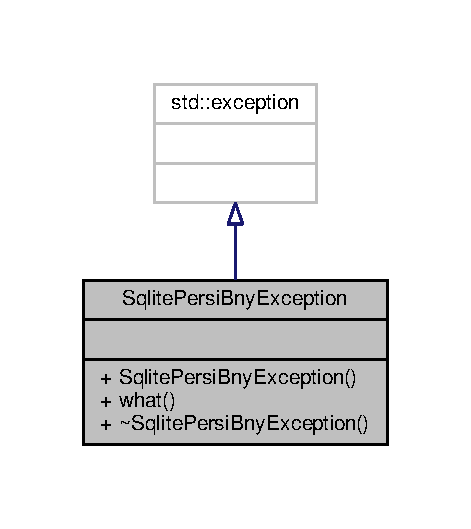
\includegraphics[width=226pt]{classSqlitePersiBnyException__inherit__graph}
\end{center}
\end{figure}


Graphe de collaboration de Sqlite\+Persi\+Bny\+Exception\+:\nopagebreak
\begin{figure}[H]
\begin{center}
\leavevmode
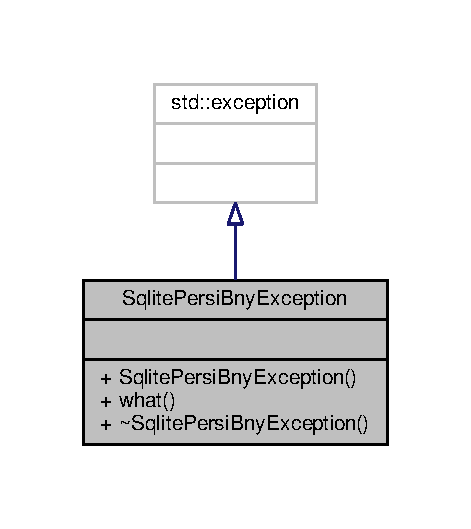
\includegraphics[width=226pt]{classSqlitePersiBnyException__coll__graph}
\end{center}
\end{figure}
\subsection*{Fonctions membres publiques}
\begin{DoxyCompactItemize}
\item 
\hyperlink{classSqlitePersiBnyException_a1bbe22eddb62428cc431146e4692406e}{Sqlite\+Persi\+Bny\+Exception} (const std\+::string description, int code)
\item 
const char $\ast$ \hyperlink{classSqlitePersiBnyException_ac1ff5b82a1a2f3ff35b1c90ddc7356d7}{what} () const  throw ()
\item 
virtual \hyperlink{classSqlitePersiBnyException_a06ed1843ac6330bb56476b28322e0836}{$\sim$\+Sqlite\+Persi\+Bny\+Exception} ()  throw ()
\end{DoxyCompactItemize}


\subsection{Documentation des constructeurs et destructeur}
\mbox{\Hypertarget{classSqlitePersiBnyException_a1bbe22eddb62428cc431146e4692406e}\label{classSqlitePersiBnyException_a1bbe22eddb62428cc431146e4692406e}} 
\index{Sqlite\+Persi\+Bny\+Exception@{Sqlite\+Persi\+Bny\+Exception}!Sqlite\+Persi\+Bny\+Exception@{Sqlite\+Persi\+Bny\+Exception}}
\index{Sqlite\+Persi\+Bny\+Exception@{Sqlite\+Persi\+Bny\+Exception}!Sqlite\+Persi\+Bny\+Exception@{Sqlite\+Persi\+Bny\+Exception}}
\subsubsection{\texorpdfstring{Sqlite\+Persi\+Bny\+Exception()}{SqlitePersiBnyException()}}
{\footnotesize\ttfamily Sqlite\+Persi\+Bny\+Exception\+::\+Sqlite\+Persi\+Bny\+Exception (\begin{DoxyParamCaption}\item[{const std\+::string}]{description,  }\item[{int}]{code }\end{DoxyParamCaption})\hspace{0.3cm}{\ttfamily [inline]}}

\mbox{\Hypertarget{classSqlitePersiBnyException_a06ed1843ac6330bb56476b28322e0836}\label{classSqlitePersiBnyException_a06ed1843ac6330bb56476b28322e0836}} 
\index{Sqlite\+Persi\+Bny\+Exception@{Sqlite\+Persi\+Bny\+Exception}!````~Sqlite\+Persi\+Bny\+Exception@{$\sim$\+Sqlite\+Persi\+Bny\+Exception}}
\index{````~Sqlite\+Persi\+Bny\+Exception@{$\sim$\+Sqlite\+Persi\+Bny\+Exception}!Sqlite\+Persi\+Bny\+Exception@{Sqlite\+Persi\+Bny\+Exception}}
\subsubsection{\texorpdfstring{$\sim$\+Sqlite\+Persi\+Bny\+Exception()}{~SqlitePersiBnyException()}}
{\footnotesize\ttfamily virtual Sqlite\+Persi\+Bny\+Exception\+::$\sim$\+Sqlite\+Persi\+Bny\+Exception (\begin{DoxyParamCaption}{ }\end{DoxyParamCaption}) throw  ) \hspace{0.3cm}{\ttfamily [inline]}, {\ttfamily [virtual]}}



\subsection{Documentation des fonctions membres}
\mbox{\Hypertarget{classSqlitePersiBnyException_ac1ff5b82a1a2f3ff35b1c90ddc7356d7}\label{classSqlitePersiBnyException_ac1ff5b82a1a2f3ff35b1c90ddc7356d7}} 
\index{Sqlite\+Persi\+Bny\+Exception@{Sqlite\+Persi\+Bny\+Exception}!what@{what}}
\index{what@{what}!Sqlite\+Persi\+Bny\+Exception@{Sqlite\+Persi\+Bny\+Exception}}
\subsubsection{\texorpdfstring{what()}{what()}}
{\footnotesize\ttfamily const char$\ast$ Sqlite\+Persi\+Bny\+Exception\+::what (\begin{DoxyParamCaption}{ }\end{DoxyParamCaption}) const throw  ) \hspace{0.3cm}{\ttfamily [inline]}}



La documentation de cette classe a été générée à partir du fichier suivant \+:\begin{DoxyCompactItemize}
\item 
src/\hyperlink{SqlitePersiBnyException_8h}{Sqlite\+Persi\+Bny\+Exception.\+h}\end{DoxyCompactItemize}

\hypertarget{classSUP}{}\section{Référence de la classe S\+UP}
\label{classSUP}\index{S\+UP@{S\+UP}}


{\ttfamily \#include $<$S\+U\+P.\+h$>$}



Graphe de collaboration de S\+UP\+:
\nopagebreak
\begin{figure}[H]
\begin{center}
\leavevmode
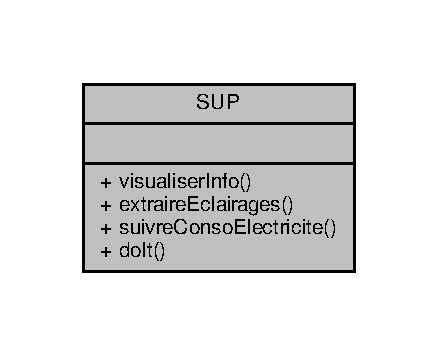
\includegraphics[width=128pt]{classSUP__coll__graph}
\end{center}
\end{figure}
\subsection*{Fonctions membres publiques}
\begin{DoxyCompactItemize}
\item 
void \hyperlink{classSUP_a00c939fd10402af9876dd3b6a0ff4abb}{do\+It} ()
\end{DoxyCompactItemize}


\subsection{Documentation des fonctions membres}
\mbox{\Hypertarget{classSUP_a00c939fd10402af9876dd3b6a0ff4abb}\label{classSUP_a00c939fd10402af9876dd3b6a0ff4abb}} 
\index{S\+UP@{S\+UP}!do\+It@{do\+It}}
\index{do\+It@{do\+It}!S\+UP@{S\+UP}}
\subsubsection{\texorpdfstring{do\+It()}{doIt()}}
{\footnotesize\ttfamily void S\+U\+P\+::do\+It (\begin{DoxyParamCaption}{ }\end{DoxyParamCaption})}



Références do\+It(), et Fichier\+Texte\+Persi\+Bny\+::get\+Contenu().



La documentation de cette classe a été générée à partir des fichiers suivants \+:\begin{DoxyCompactItemize}
\item 
src/\hyperlink{SUP_8h}{S\+U\+P.\+h}\item 
src/\hyperlink{SUP_8cpp}{S\+U\+P.\+cpp}\end{DoxyCompactItemize}

\hypertarget{classTcpComBny}{}\section{Référence de la classe Tcp\+Com\+Bny}
\label{classTcpComBny}\index{Tcp\+Com\+Bny@{Tcp\+Com\+Bny}}


{\ttfamily \#include $<$Tcp\+Com\+Bny.\+h$>$}



Graphe de collaboration de Tcp\+Com\+Bny\+:
\nopagebreak
\begin{figure}[H]
\begin{center}
\leavevmode
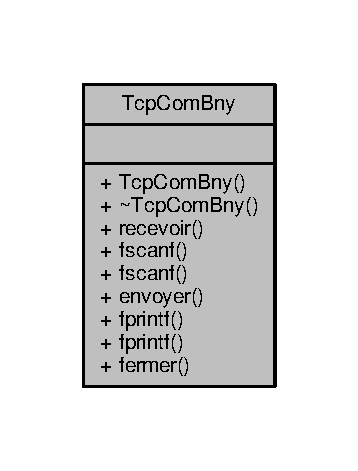
\includegraphics[width=172pt]{classTcpComBny__coll__graph}
\end{center}
\end{figure}
\subsection*{Fonctions membres publiques}
\begin{DoxyCompactItemize}
\item 
\hyperlink{classTcpComBny_a657396bbd748486fcdf0017ea49591e6}{Tcp\+Com\+Bny} (const int)  throw (\+Tcp\+Ip\+Com\+Bny\+Exception)
\item 
\hyperlink{classTcpComBny_ab4aec67058de5219876f7093c9f84353}{$\sim$\+Tcp\+Com\+Bny} ()
\item 
void \hyperlink{classTcpComBny_a1f1002ef6d3d9cfe4cfcef4cfa3ab020}{recevoir} (char $\ast$buffer, std\+::size\+\_\+t size, std\+::size\+\_\+t \&count)  throw (\+Tcp\+Ip\+Com\+Bny\+Exception)
\item 
void \hyperlink{classTcpComBny_a44a7024cd03e4fba6090026d3a1665e6}{fscanf} (const char $\ast$format,...)
\item 
void \hyperlink{classTcpComBny_a06926f8731f185ab970fa0cb687bdf28}{fscanf} (const char $\ast$format, va\+\_\+list args)
\item 
void \hyperlink{classTcpComBny_abe45becb6b9d1605e2d9433bd784024a}{envoyer} (const char $\ast$buffer, std\+::size\+\_\+t size)  throw (\+Tcp\+Ip\+Com\+Bny\+Exception)
\item 
void \hyperlink{classTcpComBny_a7ee3d2a069a30b89626793f881df6f53}{fprintf} (const char $\ast$format,...)
\item 
void \hyperlink{classTcpComBny_a9fd438f60e9c6f606ed7730c2a17a0fa}{fprintf} (const char $\ast$format, va\+\_\+list args)
\item 
void \hyperlink{classTcpComBny_a5c12a58e106149b561fd5438d1a953d2}{fermer} ()
\end{DoxyCompactItemize}


\subsection{Documentation des constructeurs et destructeur}
\mbox{\Hypertarget{classTcpComBny_a657396bbd748486fcdf0017ea49591e6}\label{classTcpComBny_a657396bbd748486fcdf0017ea49591e6}} 
\index{Tcp\+Com\+Bny@{Tcp\+Com\+Bny}!Tcp\+Com\+Bny@{Tcp\+Com\+Bny}}
\index{Tcp\+Com\+Bny@{Tcp\+Com\+Bny}!Tcp\+Com\+Bny@{Tcp\+Com\+Bny}}
\subsubsection{\texorpdfstring{Tcp\+Com\+Bny()}{TcpComBny()}}
{\footnotesize\ttfamily Tcp\+Com\+Bny\+::\+Tcp\+Com\+Bny (\begin{DoxyParamCaption}\item[{const int}]{socket\+Desc }\end{DoxyParamCaption}) throw  \hyperlink{classTcpIpComBnyException}{Tcp\+Ip\+Com\+Bny\+Exception}) }

\mbox{\Hypertarget{classTcpComBny_ab4aec67058de5219876f7093c9f84353}\label{classTcpComBny_ab4aec67058de5219876f7093c9f84353}} 
\index{Tcp\+Com\+Bny@{Tcp\+Com\+Bny}!````~Tcp\+Com\+Bny@{$\sim$\+Tcp\+Com\+Bny}}
\index{````~Tcp\+Com\+Bny@{$\sim$\+Tcp\+Com\+Bny}!Tcp\+Com\+Bny@{Tcp\+Com\+Bny}}
\subsubsection{\texorpdfstring{$\sim$\+Tcp\+Com\+Bny()}{~TcpComBny()}}
{\footnotesize\ttfamily Tcp\+Com\+Bny\+::$\sim$\+Tcp\+Com\+Bny (\begin{DoxyParamCaption}{ }\end{DoxyParamCaption})}



Références fermer().



\subsection{Documentation des fonctions membres}
\mbox{\Hypertarget{classTcpComBny_abe45becb6b9d1605e2d9433bd784024a}\label{classTcpComBny_abe45becb6b9d1605e2d9433bd784024a}} 
\index{Tcp\+Com\+Bny@{Tcp\+Com\+Bny}!envoyer@{envoyer}}
\index{envoyer@{envoyer}!Tcp\+Com\+Bny@{Tcp\+Com\+Bny}}
\subsubsection{\texorpdfstring{envoyer()}{envoyer()}}
{\footnotesize\ttfamily void Tcp\+Com\+Bny\+::envoyer (\begin{DoxyParamCaption}\item[{const char $\ast$}]{buffer,  }\item[{std\+::size\+\_\+t}]{size }\end{DoxyParamCaption}) throw  \hyperlink{classTcpIpComBnyException}{Tcp\+Ip\+Com\+Bny\+Exception}) }

\mbox{\Hypertarget{classTcpComBny_a5c12a58e106149b561fd5438d1a953d2}\label{classTcpComBny_a5c12a58e106149b561fd5438d1a953d2}} 
\index{Tcp\+Com\+Bny@{Tcp\+Com\+Bny}!fermer@{fermer}}
\index{fermer@{fermer}!Tcp\+Com\+Bny@{Tcp\+Com\+Bny}}
\subsubsection{\texorpdfstring{fermer()}{fermer()}}
{\footnotesize\ttfamily void Tcp\+Com\+Bny\+::fermer (\begin{DoxyParamCaption}{ }\end{DoxyParamCaption})}

\mbox{\Hypertarget{classTcpComBny_a7ee3d2a069a30b89626793f881df6f53}\label{classTcpComBny_a7ee3d2a069a30b89626793f881df6f53}} 
\index{Tcp\+Com\+Bny@{Tcp\+Com\+Bny}!fprintf@{fprintf}}
\index{fprintf@{fprintf}!Tcp\+Com\+Bny@{Tcp\+Com\+Bny}}
\subsubsection{\texorpdfstring{fprintf()}{fprintf()}\hspace{0.1cm}{\footnotesize\ttfamily [1/2]}}
{\footnotesize\ttfamily void Tcp\+Com\+Bny\+::fprintf (\begin{DoxyParamCaption}\item[{const char $\ast$}]{format,  }\item[{}]{... }\end{DoxyParamCaption})}

\mbox{\Hypertarget{classTcpComBny_a9fd438f60e9c6f606ed7730c2a17a0fa}\label{classTcpComBny_a9fd438f60e9c6f606ed7730c2a17a0fa}} 
\index{Tcp\+Com\+Bny@{Tcp\+Com\+Bny}!fprintf@{fprintf}}
\index{fprintf@{fprintf}!Tcp\+Com\+Bny@{Tcp\+Com\+Bny}}
\subsubsection{\texorpdfstring{fprintf()}{fprintf()}\hspace{0.1cm}{\footnotesize\ttfamily [2/2]}}
{\footnotesize\ttfamily void Tcp\+Com\+Bny\+::fprintf (\begin{DoxyParamCaption}\item[{const char $\ast$}]{format,  }\item[{va\+\_\+list}]{args }\end{DoxyParamCaption})}

\mbox{\Hypertarget{classTcpComBny_a44a7024cd03e4fba6090026d3a1665e6}\label{classTcpComBny_a44a7024cd03e4fba6090026d3a1665e6}} 
\index{Tcp\+Com\+Bny@{Tcp\+Com\+Bny}!fscanf@{fscanf}}
\index{fscanf@{fscanf}!Tcp\+Com\+Bny@{Tcp\+Com\+Bny}}
\subsubsection{\texorpdfstring{fscanf()}{fscanf()}\hspace{0.1cm}{\footnotesize\ttfamily [1/2]}}
{\footnotesize\ttfamily void Tcp\+Com\+Bny\+::fscanf (\begin{DoxyParamCaption}\item[{const char $\ast$}]{format,  }\item[{}]{... }\end{DoxyParamCaption})}

\mbox{\Hypertarget{classTcpComBny_a06926f8731f185ab970fa0cb687bdf28}\label{classTcpComBny_a06926f8731f185ab970fa0cb687bdf28}} 
\index{Tcp\+Com\+Bny@{Tcp\+Com\+Bny}!fscanf@{fscanf}}
\index{fscanf@{fscanf}!Tcp\+Com\+Bny@{Tcp\+Com\+Bny}}
\subsubsection{\texorpdfstring{fscanf()}{fscanf()}\hspace{0.1cm}{\footnotesize\ttfamily [2/2]}}
{\footnotesize\ttfamily void Tcp\+Com\+Bny\+::fscanf (\begin{DoxyParamCaption}\item[{const char $\ast$}]{format,  }\item[{va\+\_\+list}]{args }\end{DoxyParamCaption})}

\mbox{\Hypertarget{classTcpComBny_a1f1002ef6d3d9cfe4cfcef4cfa3ab020}\label{classTcpComBny_a1f1002ef6d3d9cfe4cfcef4cfa3ab020}} 
\index{Tcp\+Com\+Bny@{Tcp\+Com\+Bny}!recevoir@{recevoir}}
\index{recevoir@{recevoir}!Tcp\+Com\+Bny@{Tcp\+Com\+Bny}}
\subsubsection{\texorpdfstring{recevoir()}{recevoir()}}
{\footnotesize\ttfamily void Tcp\+Com\+Bny\+::recevoir (\begin{DoxyParamCaption}\item[{char $\ast$}]{buffer,  }\item[{std\+::size\+\_\+t}]{size,  }\item[{std\+::size\+\_\+t \&}]{count }\end{DoxyParamCaption}) throw  \hyperlink{classTcpIpComBnyException}{Tcp\+Ip\+Com\+Bny\+Exception}) }



La documentation de cette classe a été générée à partir des fichiers suivants \+:\begin{DoxyCompactItemize}
\item 
src/\hyperlink{TcpComBny_8h}{Tcp\+Com\+Bny.\+h}\item 
src/\hyperlink{TcpComBny_8cpp}{Tcp\+Com\+Bny.\+cpp}\end{DoxyCompactItemize}

\hypertarget{classTcpIpComBnyException}{}\section{Référence de la classe Tcp\+Ip\+Com\+Bny\+Exception}
\label{classTcpIpComBnyException}\index{Tcp\+Ip\+Com\+Bny\+Exception@{Tcp\+Ip\+Com\+Bny\+Exception}}


{\ttfamily \#include $<$Tcp\+Ip\+Com\+Bny\+Exception.\+h$>$}



Graphe d\textquotesingle{}héritage de Tcp\+Ip\+Com\+Bny\+Exception\+:\nopagebreak
\begin{figure}[H]
\begin{center}
\leavevmode
\includegraphics[width=224pt]{classTcpIpComBnyException__inherit__graph}
\end{center}
\end{figure}


Graphe de collaboration de Tcp\+Ip\+Com\+Bny\+Exception\+:\nopagebreak
\begin{figure}[H]
\begin{center}
\leavevmode
\includegraphics[width=224pt]{classTcpIpComBnyException__coll__graph}
\end{center}
\end{figure}
\subsection*{Fonctions membres publiques}
\begin{DoxyCompactItemize}
\item 
\hyperlink{classTcpIpComBnyException_a6ef8fb4ec6b283a18b9f4c98c2ac92d8}{Tcp\+Ip\+Com\+Bny\+Exception} (const std\+::string description)
\item 
const char $\ast$ \hyperlink{classTcpIpComBnyException_a5a5d21a18a7863b106020a2c6113402d}{what} () const  throw ()
\item 
virtual \hyperlink{classTcpIpComBnyException_a587dd6d16b9c48e652e7b3c59f2acd81}{$\sim$\+Tcp\+Ip\+Com\+Bny\+Exception} ()  throw ()
\end{DoxyCompactItemize}


\subsection{Documentation des constructeurs et destructeur}
\mbox{\Hypertarget{classTcpIpComBnyException_a6ef8fb4ec6b283a18b9f4c98c2ac92d8}\label{classTcpIpComBnyException_a6ef8fb4ec6b283a18b9f4c98c2ac92d8}} 
\index{Tcp\+Ip\+Com\+Bny\+Exception@{Tcp\+Ip\+Com\+Bny\+Exception}!Tcp\+Ip\+Com\+Bny\+Exception@{Tcp\+Ip\+Com\+Bny\+Exception}}
\index{Tcp\+Ip\+Com\+Bny\+Exception@{Tcp\+Ip\+Com\+Bny\+Exception}!Tcp\+Ip\+Com\+Bny\+Exception@{Tcp\+Ip\+Com\+Bny\+Exception}}
\subsubsection{\texorpdfstring{Tcp\+Ip\+Com\+Bny\+Exception()}{TcpIpComBnyException()}}
{\footnotesize\ttfamily Tcp\+Ip\+Com\+Bny\+Exception\+::\+Tcp\+Ip\+Com\+Bny\+Exception (\begin{DoxyParamCaption}\item[{const std\+::string}]{description }\end{DoxyParamCaption})\hspace{0.3cm}{\ttfamily [inline]}}

\mbox{\Hypertarget{classTcpIpComBnyException_a587dd6d16b9c48e652e7b3c59f2acd81}\label{classTcpIpComBnyException_a587dd6d16b9c48e652e7b3c59f2acd81}} 
\index{Tcp\+Ip\+Com\+Bny\+Exception@{Tcp\+Ip\+Com\+Bny\+Exception}!````~Tcp\+Ip\+Com\+Bny\+Exception@{$\sim$\+Tcp\+Ip\+Com\+Bny\+Exception}}
\index{````~Tcp\+Ip\+Com\+Bny\+Exception@{$\sim$\+Tcp\+Ip\+Com\+Bny\+Exception}!Tcp\+Ip\+Com\+Bny\+Exception@{Tcp\+Ip\+Com\+Bny\+Exception}}
\subsubsection{\texorpdfstring{$\sim$\+Tcp\+Ip\+Com\+Bny\+Exception()}{~TcpIpComBnyException()}}
{\footnotesize\ttfamily virtual Tcp\+Ip\+Com\+Bny\+Exception\+::$\sim$\+Tcp\+Ip\+Com\+Bny\+Exception (\begin{DoxyParamCaption}{ }\end{DoxyParamCaption}) throw  ) \hspace{0.3cm}{\ttfamily [inline]}, {\ttfamily [virtual]}}



\subsection{Documentation des fonctions membres}
\mbox{\Hypertarget{classTcpIpComBnyException_a5a5d21a18a7863b106020a2c6113402d}\label{classTcpIpComBnyException_a5a5d21a18a7863b106020a2c6113402d}} 
\index{Tcp\+Ip\+Com\+Bny\+Exception@{Tcp\+Ip\+Com\+Bny\+Exception}!what@{what}}
\index{what@{what}!Tcp\+Ip\+Com\+Bny\+Exception@{Tcp\+Ip\+Com\+Bny\+Exception}}
\subsubsection{\texorpdfstring{what()}{what()}}
{\footnotesize\ttfamily const char$\ast$ Tcp\+Ip\+Com\+Bny\+Exception\+::what (\begin{DoxyParamCaption}{ }\end{DoxyParamCaption}) const throw  ) \hspace{0.3cm}{\ttfamily [inline]}}



La documentation de cette classe a été générée à partir du fichier suivant \+:\begin{DoxyCompactItemize}
\item 
src/\hyperlink{TcpIpComBnyException_8h}{Tcp\+Ip\+Com\+Bny\+Exception.\+h}\end{DoxyCompactItemize}

\hypertarget{classUcAjouter}{}\section{Référence de la classe Uc\+Ajouter}
\label{classUcAjouter}\index{Uc\+Ajouter@{Uc\+Ajouter}}


{\ttfamily \#include $<$Uc\+Ajouter.\+h$>$}



Graphe de collaboration de Uc\+Ajouter\+:
\nopagebreak
\begin{figure}[H]
\begin{center}
\leavevmode
\includegraphics[width=140pt]{classUcAjouter__coll__graph}
\end{center}
\end{figure}
\subsection*{Fonctions membres publiques}
\begin{DoxyCompactItemize}
\item 
void \hyperlink{classUcAjouter_a8b8fd9366eba6cf693b1d4b505f4a9a2}{do\+It} (\hyperlink{classEclairageUnicolore}{Eclairage\+Unicolore} \&eclairage, cgicc\+::\+Cgicc \&cgi)
\item 
void \hyperlink{classUcAjouter_aba36b6bec074143b2733e1f5596d67d6}{do\+It} (\hyperlink{classEclairageMulticolore}{Eclairage\+Multicolore} \&eclairage, cgicc\+::\+Cgicc \&cgi)
\end{DoxyCompactItemize}


\subsection{Documentation des fonctions membres}
\mbox{\Hypertarget{classUcAjouter_a8b8fd9366eba6cf693b1d4b505f4a9a2}\label{classUcAjouter_a8b8fd9366eba6cf693b1d4b505f4a9a2}} 
\index{Uc\+Ajouter@{Uc\+Ajouter}!do\+It@{do\+It}}
\index{do\+It@{do\+It}!Uc\+Ajouter@{Uc\+Ajouter}}
\subsubsection{\texorpdfstring{do\+It()}{doIt()}\hspace{0.1cm}{\footnotesize\ttfamily [1/2]}}
{\footnotesize\ttfamily void Uc\+Ajouter\+::do\+It (\begin{DoxyParamCaption}\item[{\hyperlink{classEclairageUnicolore}{Eclairage\+Unicolore} \&}]{eclairage,  }\item[{cgicc\+::\+Cgicc \&}]{cgi }\end{DoxyParamCaption})}

M�thode permettant d\textquotesingle{}ajouter un �clairage unicolore dans la base de donn�es 

Références Eclairage\+Unicolore\+::controleur, Eclairage\+Unicolore\+::\+Controleur\+::ent, Sqlite\+Persi\+Bny\+::executer\+Sql(), et Eclairage\+::\+Ent\+::set\+I\+D().

\mbox{\Hypertarget{classUcAjouter_aba36b6bec074143b2733e1f5596d67d6}\label{classUcAjouter_aba36b6bec074143b2733e1f5596d67d6}} 
\index{Uc\+Ajouter@{Uc\+Ajouter}!do\+It@{do\+It}}
\index{do\+It@{do\+It}!Uc\+Ajouter@{Uc\+Ajouter}}
\subsubsection{\texorpdfstring{do\+It()}{doIt()}\hspace{0.1cm}{\footnotesize\ttfamily [2/2]}}
{\footnotesize\ttfamily void Uc\+Ajouter\+::do\+It (\begin{DoxyParamCaption}\item[{\hyperlink{classEclairageMulticolore}{Eclairage\+Multicolore} \&}]{eclairage,  }\item[{cgicc\+::\+Cgicc \&}]{cgi }\end{DoxyParamCaption})}

M�thode permettant d\textquotesingle{}ajouter un �clairage multicolore dans la base de donn�es. 

Références Eclairage\+Multicolore\+::controleur, do\+It(), Eclairage\+Multicolore\+::\+Controleur\+::ent, Sqlite\+Persi\+Bny\+::executer\+Sql(), et Eclairage\+::\+Ent\+::set\+I\+D().



La documentation de cette classe a été générée à partir des fichiers suivants \+:\begin{DoxyCompactItemize}
\item 
src/\hyperlink{UcAjouter_8h}{Uc\+Ajouter.\+h}\item 
src/\hyperlink{UcAjouter_8cpp}{Uc\+Ajouter.\+cpp}\end{DoxyCompactItemize}

\hypertarget{classUcCommander}{}\section{Référence de la classe Uc\+Commander}
\label{classUcCommander}\index{Uc\+Commander@{Uc\+Commander}}


{\ttfamily \#include $<$Uc\+Commander.\+h$>$}



Graphe de collaboration de Uc\+Commander\+:\nopagebreak
\begin{figure}[H]
\begin{center}
\leavevmode
\includegraphics[width=163pt]{classUcCommander__coll__graph}
\end{center}
\end{figure}
\subsection*{Fonctions membres publiques}
\begin{DoxyCompactItemize}
\item 
void \hyperlink{classUcCommander_a692e86b498f3d897f122479ec1954ed8}{do\+It} (\hyperlink{classEclairage_1_1Ent}{Eclairage\+::\+Ent} \&eclairage, bool etat)
\end{DoxyCompactItemize}


\subsection{Documentation des fonctions membres}
\mbox{\Hypertarget{classUcCommander_a692e86b498f3d897f122479ec1954ed8}\label{classUcCommander_a692e86b498f3d897f122479ec1954ed8}} 
\index{Uc\+Commander@{Uc\+Commander}!do\+It@{do\+It}}
\index{do\+It@{do\+It}!Uc\+Commander@{Uc\+Commander}}
\subsubsection{\texorpdfstring{do\+It()}{doIt()}}
{\footnotesize\ttfamily void Uc\+Commander\+::do\+It (\begin{DoxyParamCaption}\item[{\hyperlink{classEclairage_1_1Ent}{Eclairage\+::\+Ent} \&}]{eclairage,  }\item[{bool}]{etat }\end{DoxyParamCaption})}

Méthode permettant d\textquotesingle{}allumer/éteindre un éclairage passé en paramètres. 

Références Eclairage\+::controleur, do\+It(), Eclairage\+::\+Controleur\+::ent, Eclairage\+::\+Ent\+::set\+Allume(), et Eclairage\+::\+Ent\+::set\+I\+D().



La documentation de cette classe a été générée à partir des fichiers suivants \+:\begin{DoxyCompactItemize}
\item 
src/\hyperlink{UcCommander_8h}{Uc\+Commander.\+h}\item 
src/\hyperlink{UcCommander_8cpp}{Uc\+Commander.\+cpp}\end{DoxyCompactItemize}

\hypertarget{classUcExporter}{}\section{Référence de la classe Uc\+Exporter}
\label{classUcExporter}\index{Uc\+Exporter@{Uc\+Exporter}}


{\ttfamily \#include $<$Uc\+Exporter.\+h$>$}



Graphe de collaboration de Uc\+Exporter\+:
\nopagebreak
\begin{figure}[H]
\begin{center}
\leavevmode
\includegraphics[width=146pt]{classUcExporter__coll__graph}
\end{center}
\end{figure}
\subsection*{Fonctions membres publiques}
\begin{DoxyCompactItemize}
\item 
void \hyperlink{classUcExporter_ac58a112386cb857aa088359d591f043b}{do\+It} ()
\end{DoxyCompactItemize}


\subsection{Documentation des fonctions membres}
\mbox{\Hypertarget{classUcExporter_ac58a112386cb857aa088359d591f043b}\label{classUcExporter_ac58a112386cb857aa088359d591f043b}} 
\index{Uc\+Exporter@{Uc\+Exporter}!do\+It@{do\+It}}
\index{do\+It@{do\+It}!Uc\+Exporter@{Uc\+Exporter}}
\subsubsection{\texorpdfstring{do\+It()}{doIt()}}
{\footnotesize\ttfamily void Uc\+Exporter\+::do\+It (\begin{DoxyParamCaption}{ }\end{DoxyParamCaption})}

M�thode permettant d\textquotesingle{}exporter toutes les configurations d\textquotesingle{}�clairages vers un fichier \hyperlink{classCSV}{C\+SV} et de le faire t�l�charger au propri�taire depuis son navigateur W\+EB. 

Références do\+It(), et main().



La documentation de cette classe a été générée à partir des fichiers suivants \+:\begin{DoxyCompactItemize}
\item 
src/\hyperlink{UcExporter_8h}{Uc\+Exporter.\+h}\item 
src/\hyperlink{UcExporter_8cpp}{Uc\+Exporter.\+cpp}\end{DoxyCompactItemize}

\hypertarget{classUcGerer}{}\section{Référence de la classe Uc\+Gerer}
\label{classUcGerer}\index{Uc\+Gerer@{Uc\+Gerer}}


{\ttfamily \#include $<$Uc\+Gerer.\+h$>$}



Graphe de collaboration de Uc\+Gerer\+:\nopagebreak
\begin{figure}[H]
\begin{center}
\leavevmode
\includegraphics[width=133pt]{classUcGerer__coll__graph}
\end{center}
\end{figure}
\subsection*{Fonctions membres publiques}
\begin{DoxyCompactItemize}
\item 
void \hyperlink{classUcGerer_a2a1a10e0cc0d0f9bb110a87a6b8e44cb}{do\+It} (const Ent \&eclairage, bool etat)
\end{DoxyCompactItemize}


\subsection{Documentation des fonctions membres}
\mbox{\Hypertarget{classUcGerer_a2a1a10e0cc0d0f9bb110a87a6b8e44cb}\label{classUcGerer_a2a1a10e0cc0d0f9bb110a87a6b8e44cb}} 
\index{Uc\+Gerer@{Uc\+Gerer}!do\+It@{do\+It}}
\index{do\+It@{do\+It}!Uc\+Gerer@{Uc\+Gerer}}
\subsubsection{\texorpdfstring{do\+It()}{doIt()}}
{\footnotesize\ttfamily void Uc\+Gerer\+::do\+It (\begin{DoxyParamCaption}\item[{const Ent \&}]{eclairage,  }\item[{bool}]{etat }\end{DoxyParamCaption})}

M�thode permettant d\textquotesingle{}activer/desactiver un �clairage pass� en param�tre. 

La documentation de cette classe a été générée à partir des fichiers suivants \+:\begin{DoxyCompactItemize}
\item 
src/\hyperlink{UcGerer_8h}{Uc\+Gerer.\+h}\item 
src/\hyperlink{UcGerer_8cpp}{Uc\+Gerer.\+cpp}\end{DoxyCompactItemize}

\hypertarget{classUcImporter}{}\section{Référence de la classe Uc\+Importer}
\label{classUcImporter}\index{Uc\+Importer@{Uc\+Importer}}


{\ttfamily \#include $<$Uc\+Importer.\+h$>$}



Graphe de collaboration de Uc\+Importer\+:\nopagebreak
\begin{figure}[H]
\begin{center}
\leavevmode
\includegraphics[width=145pt]{classUcImporter__coll__graph}
\end{center}
\end{figure}
\subsection*{Fonctions membres publiques}
\begin{DoxyCompactItemize}
\item 
void \hyperlink{classUcImporter_a93440ab7c07ac87c4860d97e17da9080}{do\+It} (const F\+I\+LE \&fichier\+C\+SV, const \hyperlink{classUcGerer}{Uc\+Gerer} \&uc\+Gerer)
\end{DoxyCompactItemize}


\subsection{Documentation des fonctions membres}
\mbox{\Hypertarget{classUcImporter_a93440ab7c07ac87c4860d97e17da9080}\label{classUcImporter_a93440ab7c07ac87c4860d97e17da9080}} 
\index{Uc\+Importer@{Uc\+Importer}!do\+It@{do\+It}}
\index{do\+It@{do\+It}!Uc\+Importer@{Uc\+Importer}}
\subsubsection{\texorpdfstring{do\+It()}{doIt()}}
{\footnotesize\ttfamily void Uc\+Importer\+::do\+It (\begin{DoxyParamCaption}\item[{const F\+I\+LE \&}]{fichier\+C\+SV,  }\item[{const \hyperlink{classUcGerer}{Uc\+Gerer} \&}]{uc\+Gerer }\end{DoxyParamCaption})}

M�thode permettant d\textquotesingle{}importer dans la base de donn�es les configurations d\textquotesingle{}�clairages depuis un fichier au format C\+SV. 

La documentation de cette classe a été générée à partir des fichiers suivants \+:\begin{DoxyCompactItemize}
\item 
src/\hyperlink{UcImporter_8h}{Uc\+Importer.\+h}\item 
src/\hyperlink{UcImporter_8cpp}{Uc\+Importer.\+cpp}\end{DoxyCompactItemize}

\hypertarget{classUcMettreAJour}{}\section{Référence de la classe Uc\+Mettre\+A\+Jour}
\label{classUcMettreAJour}\index{Uc\+Mettre\+A\+Jour@{Uc\+Mettre\+A\+Jour}}


{\ttfamily \#include $<$Uc\+Mettre\+A\+Jour.\+h$>$}



Graphe de collaboration de Uc\+Mettre\+A\+Jour\+:
\nopagebreak
\begin{figure}[H]
\begin{center}
\leavevmode
\includegraphics[width=163pt]{classUcMettreAJour__coll__graph}
\end{center}
\end{figure}
\subsection*{Fonctions membres publiques}
\begin{DoxyCompactItemize}
\item 
void \hyperlink{classUcMettreAJour_adf3d64f62ddadb7ceaed32febd4c878d}{do\+It} (const std\+::string \&adresse\+IP, const unsigned int \&port)
\end{DoxyCompactItemize}


\subsection{Documentation des fonctions membres}
\mbox{\Hypertarget{classUcMettreAJour_adf3d64f62ddadb7ceaed32febd4c878d}\label{classUcMettreAJour_adf3d64f62ddadb7ceaed32febd4c878d}} 
\index{Uc\+Mettre\+A\+Jour@{Uc\+Mettre\+A\+Jour}!do\+It@{do\+It}}
\index{do\+It@{do\+It}!Uc\+Mettre\+A\+Jour@{Uc\+Mettre\+A\+Jour}}
\subsubsection{\texorpdfstring{do\+It()}{doIt()}}
{\footnotesize\ttfamily void Uc\+Mettre\+A\+Jour\+::do\+It (\begin{DoxyParamCaption}\item[{const std\+::string \&}]{adresse\+IP,  }\item[{const unsigned int \&}]{port }\end{DoxyParamCaption})}

M�thode permettant de mettre � jour le micrologiciel d\textquotesingle{}un �clairage multicolore. 

Références main().



La documentation de cette classe a été générée à partir des fichiers suivants \+:\begin{DoxyCompactItemize}
\item 
src/\hyperlink{UcMettreAJour_8h}{Uc\+Mettre\+A\+Jour.\+h}\item 
src/\hyperlink{UcMettreAJour_8cpp}{Uc\+Mettre\+A\+Jour.\+cpp}\end{DoxyCompactItemize}

\hypertarget{classUcModifier}{}\section{Référence de la classe Uc\+Modifier}
\label{classUcModifier}\index{Uc\+Modifier@{Uc\+Modifier}}


{\ttfamily \#include $<$Uc\+Modifier.\+h$>$}



Graphe de collaboration de Uc\+Modifier\+:
\nopagebreak
\begin{figure}[H]
\begin{center}
\leavevmode
\includegraphics[width=144pt]{classUcModifier__coll__graph}
\end{center}
\end{figure}
\subsection*{Fonctions membres publiques}
\begin{DoxyCompactItemize}
\item 
void \hyperlink{classUcModifier_a24b0e875af96b4e32a0a5085d0aaf5bb}{do\+It} (\hyperlink{classEclairageMulticolore}{Eclairage\+Multicolore} \&eclairage, cgicc\+::\+Cgicc \&cgi)
\item 
void \hyperlink{classUcModifier_a101ddb93b5cf6bf1b85cb0d0bbdaca42}{do\+It} (\hyperlink{classEclairageUnicolore}{Eclairage\+Unicolore} \&eclairage, cgicc\+::\+Cgicc \&cgi)
\end{DoxyCompactItemize}


\subsection{Documentation des fonctions membres}
\mbox{\Hypertarget{classUcModifier_a24b0e875af96b4e32a0a5085d0aaf5bb}\label{classUcModifier_a24b0e875af96b4e32a0a5085d0aaf5bb}} 
\index{Uc\+Modifier@{Uc\+Modifier}!do\+It@{do\+It}}
\index{do\+It@{do\+It}!Uc\+Modifier@{Uc\+Modifier}}
\subsubsection{\texorpdfstring{do\+It()}{doIt()}\hspace{0.1cm}{\footnotesize\ttfamily [1/2]}}
{\footnotesize\ttfamily void Uc\+Modifier\+::do\+It (\begin{DoxyParamCaption}\item[{\hyperlink{classEclairageMulticolore}{Eclairage\+Multicolore} \&}]{eclairage,  }\item[{cgicc\+::\+Cgicc \&}]{cgi }\end{DoxyParamCaption})}

M�thode permettant de modifier la configuration un �clairage multicolore. 

Références Eclairage\+Multicolore\+::\+Eclairage\+Com\+Bny\+::changer\+Couleur(), Eclairage\+Multicolore\+::controleur, Eclairage\+Multicolore\+::\+Controleur\+::eclairage\+Com\+Bny, Eclairage\+Multicolore\+::\+Controleur\+::ent, Sqlite\+Persi\+Bny\+::executer\+Sql(), Eclairage\+Multicolore\+::\+Ent\+::set\+Adresse\+I\+P(), et Eclairage\+::\+Ent\+::set\+I\+D().

\mbox{\Hypertarget{classUcModifier_a101ddb93b5cf6bf1b85cb0d0bbdaca42}\label{classUcModifier_a101ddb93b5cf6bf1b85cb0d0bbdaca42}} 
\index{Uc\+Modifier@{Uc\+Modifier}!do\+It@{do\+It}}
\index{do\+It@{do\+It}!Uc\+Modifier@{Uc\+Modifier}}
\subsubsection{\texorpdfstring{do\+It()}{doIt()}\hspace{0.1cm}{\footnotesize\ttfamily [2/2]}}
{\footnotesize\ttfamily void Uc\+Modifier\+::do\+It (\begin{DoxyParamCaption}\item[{\hyperlink{classEclairageUnicolore}{Eclairage\+Unicolore} \&}]{eclairage,  }\item[{cgicc\+::\+Cgicc \&}]{cgi }\end{DoxyParamCaption})}

M�thode permettant de modifier la configuration d\textquotesingle{}un �clairage unicolore. 

Références Eclairage\+Unicolore\+::controleur, Eclairage\+Multicolore\+::controleur, do\+It(), Eclairage\+Unicolore\+::\+Controleur\+::ent, Eclairage\+Multicolore\+::\+Controleur\+::ent, Sqlite\+Persi\+Bny\+::executer\+Sql(), et Eclairage\+::\+Ent\+::set\+I\+D().



La documentation de cette classe a été générée à partir des fichiers suivants \+:\begin{DoxyCompactItemize}
\item 
src/\hyperlink{UcModifier_8h}{Uc\+Modifier.\+h}\item 
src/\hyperlink{UcModifier_8cpp}{Uc\+Modifier.\+cpp}\end{DoxyCompactItemize}

\hypertarget{classUcSupprimer}{}\section{Référence de la classe Uc\+Supprimer}
\label{classUcSupprimer}\index{Uc\+Supprimer@{Uc\+Supprimer}}


{\ttfamily \#include $<$Uc\+Supprimer.\+h$>$}



Graphe de collaboration de Uc\+Supprimer\+:\nopagebreak
\begin{figure}[H]
\begin{center}
\leavevmode
\includegraphics[width=154pt]{classUcSupprimer__coll__graph}
\end{center}
\end{figure}
\subsection*{Fonctions membres publiques}
\begin{DoxyCompactItemize}
\item 
void \hyperlink{classUcSupprimer_af12ccac719c5584592873b3d3c6a7c3e}{do\+It} (\hyperlink{classEclairage_1_1Ent}{Eclairage\+::\+Ent} eclairage)
\end{DoxyCompactItemize}


\subsection{Documentation des fonctions membres}
\mbox{\Hypertarget{classUcSupprimer_af12ccac719c5584592873b3d3c6a7c3e}\label{classUcSupprimer_af12ccac719c5584592873b3d3c6a7c3e}} 
\index{Uc\+Supprimer@{Uc\+Supprimer}!do\+It@{do\+It}}
\index{do\+It@{do\+It}!Uc\+Supprimer@{Uc\+Supprimer}}
\subsubsection{\texorpdfstring{do\+It()}{doIt()}}
{\footnotesize\ttfamily void Uc\+Supprimer\+::do\+It (\begin{DoxyParamCaption}\item[{\hyperlink{classEclairage_1_1Ent}{Eclairage\+::\+Ent}}]{eclairage }\end{DoxyParamCaption})}

M�thode permettant de supprimer un �clairage. 

Références Eclairage\+::controleur, do\+It(), Eclairage\+::\+Controleur\+::ent, Sqlite\+Persi\+Bny\+::executer\+Sql(), Eclairage\+::\+Controleur\+::get(), Eclairage\+::\+Ent\+::get\+I\+D(), et Eclairage\+::\+Ent\+::set\+I\+D().



La documentation de cette classe a été générée à partir des fichiers suivants \+:\begin{DoxyCompactItemize}
\item 
src/\hyperlink{UcSupprimer_8h}{Uc\+Supprimer.\+h}\item 
src/\hyperlink{UcSupprimer_8cpp}{Uc\+Supprimer.\+cpp}\end{DoxyCompactItemize}

\hypertarget{classUtility}{}\section{Référence de la classe Utility}
\label{classUtility}\index{Utility@{Utility}}


{\ttfamily \#include $<$Utility.\+h$>$}



Graphe de collaboration de Utility\+:\nopagebreak
\begin{figure}[H]
\begin{center}
\leavevmode
\includegraphics[width=156pt]{classUtility__coll__graph}
\end{center}
\end{figure}
\subsection*{Fonctions membres publiques statiques}
\begin{DoxyCompactItemize}
\item 
static std\+::string \hyperlink{classUtility_a954a0d1bb807e5aa0c3d7c7d1059c5fb}{remplacer} (std\+::string, std\+::vector$<$ std\+::pair$<$ std\+::string, std\+::string $>$ $>$ \&)
\item 
static void \hyperlink{classUtility_ad60c39b61fe45ce689004b818c4b6e2b}{log\+\_\+action} (unsigned int id, std\+::string, std\+::string)
\end{DoxyCompactItemize}


\subsection{Documentation des fonctions membres}
\mbox{\Hypertarget{classUtility_ad60c39b61fe45ce689004b818c4b6e2b}\label{classUtility_ad60c39b61fe45ce689004b818c4b6e2b}} 
\index{Utility@{Utility}!log\+\_\+action@{log\+\_\+action}}
\index{log\+\_\+action@{log\+\_\+action}!Utility@{Utility}}
\subsubsection{\texorpdfstring{log\+\_\+action()}{log\_action()}}
{\footnotesize\ttfamily void Utility\+::log\+\_\+action (\begin{DoxyParamCaption}\item[{unsigned int}]{id,  }\item[{std\+::string}]{action,  }\item[{std\+::string}]{value }\end{DoxyParamCaption})\hspace{0.3cm}{\ttfamily [static]}}

Méthode permettant de loguer les actions d\textquotesingle{}un eclairage dans la table \char`\"{}logs\char`\"{} en lui indiquant l\textquotesingle{}ID de l\textquotesingle{}eclairage, son action et sa valeur 

Références Sqlite\+Persi\+Bny\+::executer\+Sql().

\mbox{\Hypertarget{classUtility_a954a0d1bb807e5aa0c3d7c7d1059c5fb}\label{classUtility_a954a0d1bb807e5aa0c3d7c7d1059c5fb}} 
\index{Utility@{Utility}!remplacer@{remplacer}}
\index{remplacer@{remplacer}!Utility@{Utility}}
\subsubsection{\texorpdfstring{remplacer()}{remplacer()}}
{\footnotesize\ttfamily std\+::string Utility\+::remplacer (\begin{DoxyParamCaption}\item[{std\+::string}]{nom\+Fichier,  }\item[{std\+::vector$<$ std\+::pair$<$ std\+::string, std\+::string $>$ $>$ \&}]{conversion }\end{DoxyParamCaption})\hspace{0.3cm}{\ttfamily [static]}}

Méthode permettant de remplacer des éléments H\+T\+ML par une pair de données (utilisé pour les infos d\textquotesingle{}éclairages) 

Références Fichier\+Texte\+Persi\+Bny\+::get\+Contenu().



La documentation de cette classe a été générée à partir des fichiers suivants \+:\begin{DoxyCompactItemize}
\item 
src/\hyperlink{Utility_8h}{Utility.\+h}\item 
src/\hyperlink{Utility_8cpp}{Utility.\+cpp}\end{DoxyCompactItemize}

\chapter{Documentation des fichiers}
\hypertarget{README_8md}{}\section{Référence du fichier R\+E\+A\+D\+M\+E.\+md}
\label{README_8md}\index{R\+E\+A\+D\+M\+E.\+md@{R\+E\+A\+D\+M\+E.\+md}}

\hypertarget{ClientTcpComBny_8cpp}{}\section{Référence du fichier src/\+Client\+Tcp\+Com\+Bny.cpp}
\label{ClientTcpComBny_8cpp}\index{src/\+Client\+Tcp\+Com\+Bny.\+cpp@{src/\+Client\+Tcp\+Com\+Bny.\+cpp}}
{\ttfamily \#include $<$cstdarg$>$}\newline
{\ttfamily \#include $<$unistd.\+h$>$}\newline
{\ttfamily \#include $<$string.\+h$>$}\newline
{\ttfamily \#include $<$sys/types.\+h$>$}\newline
{\ttfamily \#include $<$sys/socket.\+h$>$}\newline
{\ttfamily \#include $<$netinet/in.\+h$>$}\newline
{\ttfamily \#include $<$arpa/inet.\+h$>$}\newline
{\ttfamily \#include $<$Client\+Tcp\+Com\+Bny.\+h$>$}\newline
{\ttfamily \#include $<$Tcp\+Com\+Bny.\+h$>$}\newline
Graphe des dépendances par inclusion de Client\+Tcp\+Com\+Bny.\+cpp\+:\nopagebreak
\begin{figure}[H]
\begin{center}
\leavevmode
\includegraphics[width=350pt]{ClientTcpComBny_8cpp__incl}
\end{center}
\end{figure}

\hypertarget{ClientTcpComBny_8h}{}\section{Référence du fichier src/\+Client\+Tcp\+Com\+Bny.h}
\label{ClientTcpComBny_8h}\index{src/\+Client\+Tcp\+Com\+Bny.\+h@{src/\+Client\+Tcp\+Com\+Bny.\+h}}
{\ttfamily \#include $<$string$>$}\newline
{\ttfamily \#include $<$cstdarg$>$}\newline
{\ttfamily \#include $<$Tcp\+Ip\+Com\+Bny\+Exception.\+h$>$}\newline
Graphe des dépendances par inclusion de Client\+Tcp\+Com\+Bny.\+h\+:\nopagebreak
\begin{figure}[H]
\begin{center}
\leavevmode
\includegraphics[width=315pt]{ClientTcpComBny_8h__incl}
\end{center}
\end{figure}
Ce graphe montre quels fichiers incluent directement ou indirectement ce fichier \+:\nopagebreak
\begin{figure}[H]
\begin{center}
\leavevmode
\includegraphics[width=212pt]{ClientTcpComBny_8h__dep__incl}
\end{center}
\end{figure}
\subsection*{Classes}
\begin{DoxyCompactItemize}
\item 
class \hyperlink{classClientTcpComBny}{Client\+Tcp\+Com\+Bny}
\end{DoxyCompactItemize}

\hypertarget{csv_8cpp}{}\section{Référence du fichier src/csv.cpp}
\label{csv_8cpp}\index{src/csv.\+cpp@{src/csv.\+cpp}}
{\ttfamily \#include $<$iostream$>$}\newline
{\ttfamily \#include \char`\"{}csv.\+h\char`\"{}}\newline
Graphe des dépendances par inclusion de csv.\+cpp\+:
\nopagebreak
\begin{figure}[H]
\begin{center}
\leavevmode
\includegraphics[width=305pt]{csv_8cpp__incl}
\end{center}
\end{figure}

\hypertarget{csv_8h}{}\section{Référence du fichier src/csv.h}
\label{csv_8h}\index{src/csv.\+h@{src/csv.\+h}}
{\ttfamily \#include $<$map$>$}\newline
{\ttfamily \#include $<$string$>$}\newline
{\ttfamily \#include $<$vector$>$}\newline
{\ttfamily \#include $<$fstream$>$}\newline
Graphe des dépendances par inclusion de csv.\+h\+:
\nopagebreak
\begin{figure}[H]
\begin{center}
\leavevmode
\includegraphics[width=305pt]{csv_8h__incl}
\end{center}
\end{figure}
Ce graphe montre quels fichiers incluent directement ou indirectement ce fichier \+:
\nopagebreak
\begin{figure}[H]
\begin{center}
\leavevmode
\includegraphics[width=262pt]{csv_8h__dep__incl}
\end{center}
\end{figure}
\subsection*{Classes}
\begin{DoxyCompactItemize}
\item 
class \hyperlink{classCSV}{C\+SV}
\end{DoxyCompactItemize}

\hypertarget{Eclairage_8cpp}{}\section{Référence du fichier src/\+Eclairage.cpp}
\label{Eclairage_8cpp}\index{src/\+Eclairage.\+cpp@{src/\+Eclairage.\+cpp}}
{\ttfamily \#include \char`\"{}Eclairage.\+h\char`\"{}}\newline
{\ttfamily \#include \char`\"{}Uc\+Gerer.\+h\char`\"{}}\newline
Graphe des dépendances par inclusion de Eclairage.\+cpp\+:\nopagebreak
\begin{figure}[H]
\begin{center}
\leavevmode
\includegraphics[width=350pt]{Eclairage_8cpp__incl}
\end{center}
\end{figure}

\hypertarget{Eclairage_8h}{}\section{Référence du fichier src/\+Eclairage.h}
\label{Eclairage_8h}\index{src/\+Eclairage.\+h@{src/\+Eclairage.\+h}}
{\ttfamily \#include $<$string$>$}\newline
{\ttfamily \#include $<$vector$>$}\newline
{\ttfamily \#include $<$iostream$>$}\newline
{\ttfamily \#include $<$unistd.\+h$>$}\newline
{\ttfamily \#include $<$Utility.\+h$>$}\newline
{\ttfamily \#include $<$cgicc/\+Cgicc.\+h$>$}\newline
{\ttfamily \#include $<$Sqlite\+Persi\+Bny.\+h$>$}\newline
{\ttfamily \#include $<$Client\+Tcp\+Com\+Bny.\+h$>$}\newline
{\ttfamily \#include $<$cgicc/\+H\+T\+M\+L\+Classes.\+h$>$}\newline
{\ttfamily \#include $<$Fichier\+Texte\+Persi\+Bny.\+h$>$}\newline
{\ttfamily \#include $<$cgicc/\+H\+T\+T\+P\+H\+T\+M\+L\+Header.\+h$>$}\newline
Graphe des dépendances par inclusion de Eclairage.\+h\+:
\nopagebreak
\begin{figure}[H]
\begin{center}
\leavevmode
\includegraphics[width=350pt]{Eclairage_8h__incl}
\end{center}
\end{figure}
Ce graphe montre quels fichiers incluent directement ou indirectement ce fichier \+:
\nopagebreak
\begin{figure}[H]
\begin{center}
\leavevmode
\includegraphics[width=350pt]{Eclairage_8h__dep__incl}
\end{center}
\end{figure}
\subsection*{Classes}
\begin{DoxyCompactItemize}
\item 
class \hyperlink{classEclairage}{Eclairage}
\item 
class \hyperlink{classEclairage_1_1Ent}{Eclairage\+::\+Ent}
\item 
class \hyperlink{classEclairage_1_1IHMFormulaire}{Eclairage\+::\+I\+H\+M\+Formulaire}
\item 
class \hyperlink{classEclairage_1_1PersiBny}{Eclairage\+::\+Persi\+Bny}
\item 
class \hyperlink{classEclairage_1_1IHMJardin}{Eclairage\+::\+I\+H\+M\+Jardin}
\item 
class \hyperlink{classEclairage_1_1Controleur}{Eclairage\+::\+Controleur}
\end{DoxyCompactItemize}

\hypertarget{EclairageMulticolore_8cpp}{}\section{Référence du fichier src/\+Eclairage\+Multicolore.cpp}
\label{EclairageMulticolore_8cpp}\index{src/\+Eclairage\+Multicolore.\+cpp@{src/\+Eclairage\+Multicolore.\+cpp}}
{\ttfamily \#include \char`\"{}Eclairage\+Multicolore.\+h\char`\"{}}\newline
Graphe des dépendances par inclusion de Eclairage\+Multicolore.\+cpp\+:\nopagebreak
\begin{figure}[H]
\begin{center}
\leavevmode
\includegraphics[width=220pt]{EclairageMulticolore_8cpp__incl}
\end{center}
\end{figure}

\hypertarget{EclairageMulticolore_8h}{}\section{Référence du fichier src/\+Eclairage\+Multicolore.h}
\label{EclairageMulticolore_8h}\index{src/\+Eclairage\+Multicolore.\+h@{src/\+Eclairage\+Multicolore.\+h}}
{\ttfamily \#include $<$Eclairage.\+h$>$}\newline
Graphe des dépendances par inclusion de Eclairage\+Multicolore.\+h\+:
\nopagebreak
\begin{figure}[H]
\begin{center}
\leavevmode
\includegraphics[width=350pt]{EclairageMulticolore_8h__incl}
\end{center}
\end{figure}
Ce graphe montre quels fichiers incluent directement ou indirectement ce fichier \+:
\nopagebreak
\begin{figure}[H]
\begin{center}
\leavevmode
\includegraphics[width=350pt]{EclairageMulticolore_8h__dep__incl}
\end{center}
\end{figure}
\subsection*{Classes}
\begin{DoxyCompactItemize}
\item 
class \hyperlink{classEclairageMulticolore}{Eclairage\+Multicolore}
\item 
class \hyperlink{classEclairageMulticolore_1_1Ent}{Eclairage\+Multicolore\+::\+Ent}
\item 
class \hyperlink{classEclairageMulticolore_1_1PersiBny}{Eclairage\+Multicolore\+::\+Persi\+Bny}
\item 
class \hyperlink{classEclairageMulticolore_1_1IHMFormulaire}{Eclairage\+Multicolore\+::\+I\+H\+M\+Formulaire}
\item 
class \hyperlink{classEclairageMulticolore_1_1IHMJardin}{Eclairage\+Multicolore\+::\+I\+H\+M\+Jardin}
\item 
class \hyperlink{classEclairageMulticolore_1_1IHMParametre}{Eclairage\+Multicolore\+::\+I\+H\+M\+Parametre}
\item 
class \hyperlink{classEclairageMulticolore_1_1Controleur}{Eclairage\+Multicolore\+::\+Controleur}
\end{DoxyCompactItemize}

\hypertarget{EclairageUnicolore_8cpp}{}\section{Référence du fichier src/\+Eclairage\+Unicolore.cpp}
\label{EclairageUnicolore_8cpp}\index{src/\+Eclairage\+Unicolore.\+cpp@{src/\+Eclairage\+Unicolore.\+cpp}}
{\ttfamily \#include $<$Eclairage\+Unicolore.\+h$>$}\newline
Graphe des dépendances par inclusion de Eclairage\+Unicolore.\+cpp\+:
\nopagebreak
\begin{figure}[H]
\begin{center}
\leavevmode
\includegraphics[width=350pt]{EclairageUnicolore_8cpp__incl}
\end{center}
\end{figure}

\hypertarget{EclairageUnicolore_8h}{}\section{Référence du fichier src/\+Eclairage\+Unicolore.h}
\label{EclairageUnicolore_8h}\index{src/\+Eclairage\+Unicolore.\+h@{src/\+Eclairage\+Unicolore.\+h}}
{\ttfamily \#include $<$Eclairage.\+h$>$}\newline
{\ttfamily \#include $<$Client\+Tcp\+Com\+Bny.\+h$>$}\newline
Graphe des dépendances par inclusion de Eclairage\+Unicolore.\+h\+:
\nopagebreak
\begin{figure}[H]
\begin{center}
\leavevmode
\includegraphics[width=350pt]{EclairageUnicolore_8h__incl}
\end{center}
\end{figure}
Ce graphe montre quels fichiers incluent directement ou indirectement ce fichier \+:
\nopagebreak
\begin{figure}[H]
\begin{center}
\leavevmode
\includegraphics[width=350pt]{EclairageUnicolore_8h__dep__incl}
\end{center}
\end{figure}
\subsection*{Classes}
\begin{DoxyCompactItemize}
\item 
class \hyperlink{classEclairageUnicolore}{Eclairage\+Unicolore}
\item 
class \hyperlink{classEclairageUnicolore_1_1Ent}{Eclairage\+Unicolore\+::\+Ent}
\item 
class \hyperlink{classEclairageUnicolore_1_1PersiBny}{Eclairage\+Unicolore\+::\+Persi\+Bny}
\item 
class \hyperlink{classEclairageUnicolore_1_1IHMFormulaire}{Eclairage\+Unicolore\+::\+I\+H\+M\+Formulaire}
\item 
class \hyperlink{classEclairageUnicolore_1_1IHMJardin}{Eclairage\+Unicolore\+::\+I\+H\+M\+Jardin}
\item 
class \hyperlink{classEclairageUnicolore_1_1IHMParametre}{Eclairage\+Unicolore\+::\+I\+H\+M\+Parametre}
\item 
class \hyperlink{classEclairageUnicolore_1_1EclairageComBny}{Eclairage\+Unicolore\+::\+Eclairage\+Com\+Bny}
\item 
class \hyperlink{classEclairageUnicolore_1_1Controleur}{Eclairage\+Unicolore\+::\+Controleur}
\end{DoxyCompactItemize}

\hypertarget{FichierTextePersiBny_8cpp}{}\section{Référence du fichier src/\+Fichier\+Texte\+Persi\+Bny.cpp}
\label{FichierTextePersiBny_8cpp}\index{src/\+Fichier\+Texte\+Persi\+Bny.\+cpp@{src/\+Fichier\+Texte\+Persi\+Bny.\+cpp}}
{\ttfamily \#include \char`\"{}Fichier\+Texte\+Persi\+Bny.\+h\char`\"{}}\newline
Graphe des dépendances par inclusion de Fichier\+Texte\+Persi\+Bny.\+cpp\+:
\nopagebreak
\begin{figure}[H]
\begin{center}
\leavevmode
\includegraphics[width=272pt]{FichierTextePersiBny_8cpp__incl}
\end{center}
\end{figure}

\hypertarget{FichierTextePersiBny_8h}{}\section{Référence du fichier src/\+Fichier\+Texte\+Persi\+Bny.h}
\label{FichierTextePersiBny_8h}\index{src/\+Fichier\+Texte\+Persi\+Bny.\+h@{src/\+Fichier\+Texte\+Persi\+Bny.\+h}}
{\ttfamily \#include $<$fstream$>$}\newline
{\ttfamily \#include $<$sstream$>$}\newline
{\ttfamily \#include $<$iostream$>$}\newline
Graphe des dépendances par inclusion de Fichier\+Texte\+Persi\+Bny.\+h\+:
\nopagebreak
\begin{figure}[H]
\begin{center}
\leavevmode
\includegraphics[width=272pt]{FichierTextePersiBny_8h__incl}
\end{center}
\end{figure}
Ce graphe montre quels fichiers incluent directement ou indirectement ce fichier \+:
\nopagebreak
\begin{figure}[H]
\begin{center}
\leavevmode
\includegraphics[width=350pt]{FichierTextePersiBny_8h__dep__incl}
\end{center}
\end{figure}
\subsection*{Classes}
\begin{DoxyCompactItemize}
\item 
class \hyperlink{classFichierTextePersiBny}{Fichier\+Texte\+Persi\+Bny}
\end{DoxyCompactItemize}

\hypertarget{SqlitePersiBny_8cpp}{}\section{Référence du fichier src/\+Sqlite\+Persi\+Bny.cpp}
\label{SqlitePersiBny_8cpp}\index{src/\+Sqlite\+Persi\+Bny.\+cpp@{src/\+Sqlite\+Persi\+Bny.\+cpp}}
{\ttfamily \#include $<$Sqlite\+Persi\+Bny.\+h$>$}\newline
{\ttfamily \#include $<$iostream$>$}\newline
{\ttfamily \#include $<$unistd.\+h$>$}\newline
{\ttfamily \#include $<$sstream$>$}\newline
Graphe des dépendances par inclusion de Sqlite\+Persi\+Bny.\+cpp\+:
\nopagebreak
\begin{figure}[H]
\begin{center}
\leavevmode
\includegraphics[width=350pt]{SqlitePersiBny_8cpp__incl}
\end{center}
\end{figure}

\hypertarget{SqlitePersiBny_8h}{}\section{Référence du fichier src/\+Sqlite\+Persi\+Bny.h}
\label{SqlitePersiBny_8h}\index{src/\+Sqlite\+Persi\+Bny.\+h@{src/\+Sqlite\+Persi\+Bny.\+h}}
{\ttfamily \#include $<$sqlite3.\+h$>$}\newline
{\ttfamily \#include $<$Sqlite\+Persi\+Bny\+Exception.\+h$>$}\newline
{\ttfamily \#include $<$vector$>$}\newline
{\ttfamily \#include $<$utility$>$}\newline
Graphe des dépendances par inclusion de Sqlite\+Persi\+Bny.\+h\+:\nopagebreak
\begin{figure}[H]
\begin{center}
\leavevmode
\includegraphics[width=350pt]{SqlitePersiBny_8h__incl}
\end{center}
\end{figure}
Ce graphe montre quels fichiers incluent directement ou indirectement ce fichier \+:\nopagebreak
\begin{figure}[H]
\begin{center}
\leavevmode
\includegraphics[width=350pt]{SqlitePersiBny_8h__dep__incl}
\end{center}
\end{figure}
\subsection*{Classes}
\begin{DoxyCompactItemize}
\item 
class \hyperlink{classSqlitePersiBny}{Sqlite\+Persi\+Bny}
\end{DoxyCompactItemize}

\hypertarget{SqlitePersiBnyException_8cpp}{}\section{Référence du fichier src/\+Sqlite\+Persi\+Bny\+Exception.cpp}
\label{SqlitePersiBnyException_8cpp}\index{src/\+Sqlite\+Persi\+Bny\+Exception.\+cpp@{src/\+Sqlite\+Persi\+Bny\+Exception.\+cpp}}
{\ttfamily \#include $<$Sqlite\+Persi\+Bny\+Exception.\+h$>$}\newline
Graphe des dépendances par inclusion de Sqlite\+Persi\+Bny\+Exception.\+cpp\+:\nopagebreak
\begin{figure}[H]
\begin{center}
\leavevmode
\includegraphics[width=269pt]{SqlitePersiBnyException_8cpp__incl}
\end{center}
\end{figure}

\hypertarget{SqlitePersiBnyException_8h}{}\section{Référence du fichier src/\+Sqlite\+Persi\+Bny\+Exception.h}
\label{SqlitePersiBnyException_8h}\index{src/\+Sqlite\+Persi\+Bny\+Exception.\+h@{src/\+Sqlite\+Persi\+Bny\+Exception.\+h}}
{\ttfamily \#include $<$string$>$}\newline
{\ttfamily \#include $<$exception$>$}\newline
{\ttfamily \#include $<$sqlite3.\+h$>$}\newline
Graphe des dépendances par inclusion de Sqlite\+Persi\+Bny\+Exception.\+h\+:
\nopagebreak
\begin{figure}[H]
\begin{center}
\leavevmode
\includegraphics[width=269pt]{SqlitePersiBnyException_8h__incl}
\end{center}
\end{figure}
Ce graphe montre quels fichiers incluent directement ou indirectement ce fichier \+:
\nopagebreak
\begin{figure}[H]
\begin{center}
\leavevmode
\includegraphics[width=350pt]{SqlitePersiBnyException_8h__dep__incl}
\end{center}
\end{figure}
\subsection*{Classes}
\begin{DoxyCompactItemize}
\item 
class \hyperlink{classSqlitePersiBnyException}{Sqlite\+Persi\+Bny\+Exception}
\end{DoxyCompactItemize}

\hypertarget{SUP_8cpp}{}\section{Référence du fichier src/\+S\+UP.cpp}
\label{SUP_8cpp}\index{src/\+S\+U\+P.\+cpp@{src/\+S\+U\+P.\+cpp}}
{\ttfamily \#include \char`\"{}S\+U\+P.\+h\char`\"{}}\newline
{\ttfamily \#include \char`\"{}Eclairage\+Unicolore.\+h\char`\"{}}\newline
{\ttfamily \#include \char`\"{}Eclairage\+Multicolore.\+h\char`\"{}}\newline
{\ttfamily \#include \char`\"{}Uc\+Modifier.\+h\char`\"{}}\newline
{\ttfamily \#include \char`\"{}Uc\+Ajouter.\+h\char`\"{}}\newline
{\ttfamily \#include \char`\"{}Uc\+Supprimer.\+h\char`\"{}}\newline
Graphe des dépendances par inclusion de S\+U\+P.\+cpp\+:\nopagebreak
\begin{figure}[H]
\begin{center}
\leavevmode
\includegraphics[width=350pt]{SUP_8cpp__incl}
\end{center}
\end{figure}

\hypertarget{SUP_8h}{}\section{Référence du fichier src/\+S\+UP.h}
\label{SUP_8h}\index{src/\+S\+U\+P.\+h@{src/\+S\+U\+P.\+h}}
{\ttfamily \#include $<$vector$>$}\newline
{\ttfamily \#include $<$Eclairage.\+h$>$}\newline
{\ttfamily \#include $<$Sqlite\+Persi\+Bny.\+h$>$}\newline
{\ttfamily \#include $<$Eclairage\+Unicolore.\+h$>$}\newline
{\ttfamily \#include $<$Eclairage\+Multicolore.\+h$>$}\newline
{\ttfamily \#include $<$Fichier\+Texte\+Persi\+Bny.\+h$>$}\newline
{\ttfamily \#include $<$cgicc/\+Cgi\+Defs.\+h$>$}\newline
{\ttfamily \#include $<$cgicc/\+Cgicc.\+h$>$}\newline
{\ttfamily \#include $<$cgicc/\+H\+T\+T\+P\+H\+T\+M\+L\+Header.\+h$>$}\newline
{\ttfamily \#include $<$cgicc/\+H\+T\+M\+L\+Classes.\+h$>$}\newline
{\ttfamily \#include $<$Utility.\+h$>$}\newline
Graphe des dépendances par inclusion de S\+U\+P.\+h\+:
\nopagebreak
\begin{figure}[H]
\begin{center}
\leavevmode
\includegraphics[width=350pt]{SUP_8h__incl}
\end{center}
\end{figure}
Ce graphe montre quels fichiers incluent directement ou indirectement ce fichier \+:
\nopagebreak
\begin{figure}[H]
\begin{center}
\leavevmode
\includegraphics[width=153pt]{SUP_8h__dep__incl}
\end{center}
\end{figure}
\subsection*{Classes}
\begin{DoxyCompactItemize}
\item 
class \hyperlink{classSUP}{S\+UP}
\end{DoxyCompactItemize}

\hypertarget{TcpComBny_8cpp}{}\section{Référence du fichier src/\+Tcp\+Com\+Bny.cpp}
\label{TcpComBny_8cpp}\index{src/\+Tcp\+Com\+Bny.\+cpp@{src/\+Tcp\+Com\+Bny.\+cpp}}
{\ttfamily \#include $<$Tcp\+Com\+Bny.\+h$>$}\newline
{\ttfamily \#include $<$string$>$}\newline
{\ttfamily \#include $<$cstddef$>$}\newline
{\ttfamily \#include $<$cstdio$>$}\newline
{\ttfamily \#include $<$unistd.\+h$>$}\newline
{\ttfamily \#include $<$string.\+h$>$}\newline
{\ttfamily \#include $<$sys/types.\+h$>$}\newline
{\ttfamily \#include $<$sys/socket.\+h$>$}\newline
{\ttfamily \#include $<$netinet/in.\+h$>$}\newline
{\ttfamily \#include $<$arpa/inet.\+h$>$}\newline
Graphe des dépendances par inclusion de Tcp\+Com\+Bny.\+cpp\+:\nopagebreak
\begin{figure}[H]
\begin{center}
\leavevmode
\includegraphics[width=350pt]{TcpComBny_8cpp__incl}
\end{center}
\end{figure}

\hypertarget{TcpComBny_8h}{}\section{Référence du fichier src/\+Tcp\+Com\+Bny.h}
\label{TcpComBny_8h}\index{src/\+Tcp\+Com\+Bny.\+h@{src/\+Tcp\+Com\+Bny.\+h}}
{\ttfamily \#include $<$cstdarg$>$}\newline
{\ttfamily \#include $<$Tcp\+Ip\+Com\+Bny\+Exception.\+h$>$}\newline
Graphe des dépendances par inclusion de Tcp\+Com\+Bny.\+h\+:
\nopagebreak
\begin{figure}[H]
\begin{center}
\leavevmode
\includegraphics[width=278pt]{TcpComBny_8h__incl}
\end{center}
\end{figure}
Ce graphe montre quels fichiers incluent directement ou indirectement ce fichier \+:
\nopagebreak
\begin{figure}[H]
\begin{center}
\leavevmode
\includegraphics[width=338pt]{TcpComBny_8h__dep__incl}
\end{center}
\end{figure}
\subsection*{Classes}
\begin{DoxyCompactItemize}
\item 
class \hyperlink{classTcpComBny}{Tcp\+Com\+Bny}
\end{DoxyCompactItemize}

\hypertarget{TcpIpComBnyException_8cpp}{}\section{Référence du fichier src/\+Tcp\+Ip\+Com\+Bny\+Exception.cpp}
\label{TcpIpComBnyException_8cpp}\index{src/\+Tcp\+Ip\+Com\+Bny\+Exception.\+cpp@{src/\+Tcp\+Ip\+Com\+Bny\+Exception.\+cpp}}
{\ttfamily \#include $<$Tcp\+Ip\+Com\+Bny\+Exception.\+h$>$}\newline
Graphe des dépendances par inclusion de Tcp\+Ip\+Com\+Bny\+Exception.\+cpp\+:
\nopagebreak
\begin{figure}[H]
\begin{center}
\leavevmode
\includegraphics[width=238pt]{TcpIpComBnyException_8cpp__incl}
\end{center}
\end{figure}

\hypertarget{TcpIpComBnyException_8h}{}\section{Référence du fichier src/\+Tcp\+Ip\+Com\+Bny\+Exception.h}
\label{TcpIpComBnyException_8h}\index{src/\+Tcp\+Ip\+Com\+Bny\+Exception.\+h@{src/\+Tcp\+Ip\+Com\+Bny\+Exception.\+h}}
{\ttfamily \#include $<$string$>$}\newline
{\ttfamily \#include $<$exception$>$}\newline
Graphe des dépendances par inclusion de Tcp\+Ip\+Com\+Bny\+Exception.\+h\+:\nopagebreak
\begin{figure}[H]
\begin{center}
\leavevmode
\includegraphics[width=228pt]{TcpIpComBnyException_8h__incl}
\end{center}
\end{figure}
Ce graphe montre quels fichiers incluent directement ou indirectement ce fichier \+:\nopagebreak
\begin{figure}[H]
\begin{center}
\leavevmode
\includegraphics[width=350pt]{TcpIpComBnyException_8h__dep__incl}
\end{center}
\end{figure}
\subsection*{Classes}
\begin{DoxyCompactItemize}
\item 
class \hyperlink{classTcpIpComBnyException}{Tcp\+Ip\+Com\+Bny\+Exception}
\end{DoxyCompactItemize}

\hypertarget{UcAjouter_8cpp}{}\section{Référence du fichier src/\+Uc\+Ajouter.cpp}
\label{UcAjouter_8cpp}\index{src/\+Uc\+Ajouter.\+cpp@{src/\+Uc\+Ajouter.\+cpp}}
{\ttfamily \#include \char`\"{}Uc\+Ajouter.\+h\char`\"{}}\newline
Graphe des dépendances par inclusion de Uc\+Ajouter.\+cpp\+:\nopagebreak
\begin{figure}[H]
\begin{center}
\leavevmode
\includegraphics[width=350pt]{UcAjouter_8cpp__incl}
\end{center}
\end{figure}

\hypertarget{UcAjouter_8h}{}\section{Référence du fichier src/\+Uc\+Ajouter.h}
\label{UcAjouter_8h}\index{src/\+Uc\+Ajouter.\+h@{src/\+Uc\+Ajouter.\+h}}
{\ttfamily \#include $<$vector$>$}\newline
{\ttfamily \#include $<$string$>$}\newline
{\ttfamily \#include $<$iostream$>$}\newline
{\ttfamily \#include $<$cgicc/\+Cgicc.\+h$>$}\newline
{\ttfamily \#include $<$Sqlite\+Persi\+Bny.\+h$>$}\newline
{\ttfamily \#include $<$cgicc/\+H\+T\+M\+L\+Classes.\+h$>$}\newline
{\ttfamily \#include $<$Eclairage\+Unicolore.\+h$>$}\newline
{\ttfamily \#include $<$cgicc/\+H\+T\+T\+P\+H\+T\+M\+L\+Header.\+h$>$}\newline
{\ttfamily \#include $<$Eclairage\+Multicolore.\+h$>$}\newline
Graphe des dépendances par inclusion de Uc\+Ajouter.\+h\+:
\nopagebreak
\begin{figure}[H]
\begin{center}
\leavevmode
\includegraphics[width=350pt]{UcAjouter_8h__incl}
\end{center}
\end{figure}
Ce graphe montre quels fichiers incluent directement ou indirectement ce fichier \+:
\nopagebreak
\begin{figure}[H]
\begin{center}
\leavevmode
\includegraphics[width=289pt]{UcAjouter_8h__dep__incl}
\end{center}
\end{figure}
\subsection*{Classes}
\begin{DoxyCompactItemize}
\item 
class \hyperlink{classUcAjouter}{Uc\+Ajouter}
\end{DoxyCompactItemize}

\hypertarget{UcCommander_8cpp}{}\section{Référence du fichier src/\+Uc\+Commander.cpp}
\label{UcCommander_8cpp}\index{src/\+Uc\+Commander.\+cpp@{src/\+Uc\+Commander.\+cpp}}
{\ttfamily \#include $<$Uc\+Commander.\+h$>$}\newline
Graphe des dépendances par inclusion de Uc\+Commander.\+cpp\+:
\nopagebreak
\begin{figure}[H]
\begin{center}
\leavevmode
\includegraphics[width=350pt]{UcCommander_8cpp__incl}
\end{center}
\end{figure}

\hypertarget{UcCommander_8h}{}\section{Référence du fichier src/\+Uc\+Commander.h}
\label{UcCommander_8h}\index{src/\+Uc\+Commander.\+h@{src/\+Uc\+Commander.\+h}}
Ce graphe montre quels fichiers incluent directement ou indirectement ce fichier \+:\nopagebreak
\begin{figure}[H]
\begin{center}
\leavevmode
\includegraphics[width=284pt]{UcCommander_8h__dep__incl}
\end{center}
\end{figure}
\subsection*{Classes}
\begin{DoxyCompactItemize}
\item 
class \hyperlink{classUcCommander}{Uc\+Commander}
\end{DoxyCompactItemize}

\hypertarget{UcExporter_8cpp}{}\section{Référence du fichier src/\+Uc\+Exporter.cpp}
\label{UcExporter_8cpp}\index{src/\+Uc\+Exporter.\+cpp@{src/\+Uc\+Exporter.\+cpp}}
{\ttfamily \#include \char`\"{}Uc\+Exporter.\+h\char`\"{}}\newline
Graphe des dépendances par inclusion de Uc\+Exporter.\+cpp\+:\nopagebreak
\begin{figure}[H]
\begin{center}
\leavevmode
\includegraphics[width=181pt]{UcExporter_8cpp__incl}
\end{center}
\end{figure}

\hypertarget{UcExporter_8h}{}\section{Référence du fichier src/\+Uc\+Exporter.h}
\label{UcExporter_8h}\index{src/\+Uc\+Exporter.\+h@{src/\+Uc\+Exporter.\+h}}
{\ttfamily \#include $<$iostream$>$}\newline
{\ttfamily \#include $<$cgicc/\+Cgi\+Defs.\+h$>$}\newline
{\ttfamily \#include $<$cgicc/\+Cgicc.\+h$>$}\newline
{\ttfamily \#include $<$cgicc/\+H\+T\+T\+P\+H\+T\+M\+L\+Header.\+h$>$}\newline
{\ttfamily \#include $<$cgicc/\+H\+T\+M\+L\+Classes.\+h$>$}\newline
Graphe des dépendances par inclusion de Uc\+Exporter.\+h\+:
\nopagebreak
\begin{figure}[H]
\begin{center}
\leavevmode
\includegraphics[width=350pt]{UcExporter_8h__incl}
\end{center}
\end{figure}
Ce graphe montre quels fichiers incluent directement ou indirectement ce fichier \+:
\nopagebreak
\begin{figure}[H]
\begin{center}
\leavevmode
\includegraphics[width=181pt]{UcExporter_8h__dep__incl}
\end{center}
\end{figure}
\subsection*{Classes}
\begin{DoxyCompactItemize}
\item 
class \hyperlink{classUcExporter}{Uc\+Exporter}
\end{DoxyCompactItemize}

\hypertarget{UcGerer_8cpp}{}\section{Référence du fichier src/\+Uc\+Gerer.cpp}
\label{UcGerer_8cpp}\index{src/\+Uc\+Gerer.\+cpp@{src/\+Uc\+Gerer.\+cpp}}
{\ttfamily \#include $<$Uc\+Gerer.\+h$>$}\newline
Graphe des dépendances par inclusion de Uc\+Gerer.\+cpp\+:
\nopagebreak
\begin{figure}[H]
\begin{center}
\leavevmode
\includegraphics[width=350pt]{UcGerer_8cpp__incl}
\end{center}
\end{figure}

\hypertarget{UcGerer_8h}{}\section{Référence du fichier src/\+Uc\+Gerer.h}
\label{UcGerer_8h}\index{src/\+Uc\+Gerer.\+h@{src/\+Uc\+Gerer.\+h}}
{\ttfamily \#include $<$Eclairage.\+h$>$}\newline
{\ttfamily \#include $<$iostream$>$}\newline
{\ttfamily \#include $<$cgicc/\+Cgi\+Defs.\+h$>$}\newline
{\ttfamily \#include $<$cgicc/\+Cgicc.\+h$>$}\newline
{\ttfamily \#include $<$cgicc/\+H\+T\+T\+P\+H\+T\+M\+L\+Header.\+h$>$}\newline
{\ttfamily \#include $<$cgicc/\+H\+T\+M\+L\+Classes.\+h$>$}\newline
Graphe des dépendances par inclusion de Uc\+Gerer.\+h\+:
\nopagebreak
\begin{figure}[H]
\begin{center}
\leavevmode
\includegraphics[width=350pt]{UcGerer_8h__incl}
\end{center}
\end{figure}
Ce graphe montre quels fichiers incluent directement ou indirectement ce fichier \+:
\nopagebreak
\begin{figure}[H]
\begin{center}
\leavevmode
\includegraphics[width=169pt]{UcGerer_8h__dep__incl}
\end{center}
\end{figure}
\subsection*{Classes}
\begin{DoxyCompactItemize}
\item 
class \hyperlink{classUcGerer}{Uc\+Gerer}
\end{DoxyCompactItemize}

\hypertarget{UcImporter_8cpp}{}\section{Référence du fichier src/\+Uc\+Importer.cpp}
\label{UcImporter_8cpp}\index{src/\+Uc\+Importer.\+cpp@{src/\+Uc\+Importer.\+cpp}}
{\ttfamily \#include $<$Uc\+Importer.\+h$>$}\newline
Graphe des dépendances par inclusion de Uc\+Importer.\+cpp\+:
\nopagebreak
\begin{figure}[H]
\begin{center}
\leavevmode
\includegraphics[width=350pt]{UcImporter_8cpp__incl}
\end{center}
\end{figure}

\hypertarget{UcImporter_8h}{}\section{Référence du fichier src/\+Uc\+Importer.h}
\label{UcImporter_8h}\index{src/\+Uc\+Importer.\+h@{src/\+Uc\+Importer.\+h}}
{\ttfamily \#include $<$Uc\+Modifier.\+h$>$}\newline
{\ttfamily \#include $<$Uc\+Ajouter.\+h$>$}\newline
{\ttfamily \#include $<$Sqlite\+Persi\+Bny.\+h$>$}\newline
{\ttfamily \#include $<$Eclairage.\+h$>$}\newline
{\ttfamily \#include $<$csv.\+h$>$}\newline
{\ttfamily \#include $<$new$>$}\newline
{\ttfamily \#include $<$string$>$}\newline
{\ttfamily \#include $<$vector$>$}\newline
{\ttfamily \#include $<$stdexcept$>$}\newline
{\ttfamily \#include $<$iostream$>$}\newline
{\ttfamily \#include $<$fstream$>$}\newline
{\ttfamily \#include $<$cstdio$>$}\newline
{\ttfamily \#include $<$cstdlib$>$}\newline
{\ttfamily \#include $<$cgicc/\+Cgi\+Defs.\+h$>$}\newline
{\ttfamily \#include $<$cgicc/\+Cgicc.\+h$>$}\newline
{\ttfamily \#include $<$cgicc/\+H\+T\+T\+P\+H\+T\+M\+L\+Header.\+h$>$}\newline
{\ttfamily \#include $<$cgicc/\+H\+T\+M\+L\+Classes.\+h$>$}\newline
Graphe des dépendances par inclusion de Uc\+Importer.\+h\+:
\nopagebreak
\begin{figure}[H]
\begin{center}
\leavevmode
\includegraphics[width=350pt]{UcImporter_8h__incl}
\end{center}
\end{figure}
Ce graphe montre quels fichiers incluent directement ou indirectement ce fichier \+:
\nopagebreak
\begin{figure}[H]
\begin{center}
\leavevmode
\includegraphics[width=181pt]{UcImporter_8h__dep__incl}
\end{center}
\end{figure}
\subsection*{Classes}
\begin{DoxyCompactItemize}
\item 
class \hyperlink{classUcImporter}{Uc\+Importer}
\end{DoxyCompactItemize}

\hypertarget{UcMettreAJour_8cpp}{}\section{Référence du fichier src/\+Uc\+Mettre\+A\+Jour.cpp}
\label{UcMettreAJour_8cpp}\index{src/\+Uc\+Mettre\+A\+Jour.\+cpp@{src/\+Uc\+Mettre\+A\+Jour.\+cpp}}
{\ttfamily \#include \char`\"{}Uc\+Mettre\+A\+Jour.\+h\char`\"{}}\newline
Graphe des dépendances par inclusion de Uc\+Mettre\+A\+Jour.\+cpp\+:\nopagebreak
\begin{figure}[H]
\begin{center}
\leavevmode
\includegraphics[width=198pt]{UcMettreAJour_8cpp__incl}
\end{center}
\end{figure}

\hypertarget{UcMettreAJour_8h}{}\section{Référence du fichier src/\+Uc\+Mettre\+A\+Jour.h}
\label{UcMettreAJour_8h}\index{src/\+Uc\+Mettre\+A\+Jour.\+h@{src/\+Uc\+Mettre\+A\+Jour.\+h}}
{\ttfamily \#include $<$string$>$}\newline
{\ttfamily \#include $<$Client\+Tcp\+Com\+Bny.\+h$>$}\newline
Graphe des dépendances par inclusion de Uc\+Mettre\+A\+Jour.\+h\+:
\nopagebreak
\begin{figure}[H]
\begin{center}
\leavevmode
\includegraphics[width=350pt]{UcMettreAJour_8h__incl}
\end{center}
\end{figure}
Ce graphe montre quels fichiers incluent directement ou indirectement ce fichier \+:
\nopagebreak
\begin{figure}[H]
\begin{center}
\leavevmode
\includegraphics[width=198pt]{UcMettreAJour_8h__dep__incl}
\end{center}
\end{figure}
\subsection*{Classes}
\begin{DoxyCompactItemize}
\item 
class \hyperlink{classUcMettreAJour}{Uc\+Mettre\+A\+Jour}
\end{DoxyCompactItemize}

\hypertarget{UcModifier_8cpp}{}\section{Référence du fichier src/\+Uc\+Modifier.cpp}
\label{UcModifier_8cpp}\index{src/\+Uc\+Modifier.\+cpp@{src/\+Uc\+Modifier.\+cpp}}
{\ttfamily \#include \char`\"{}Uc\+Modifier.\+h\char`\"{}}\newline
Graphe des dépendances par inclusion de Uc\+Modifier.\+cpp\+:\nopagebreak
\begin{figure}[H]
\begin{center}
\leavevmode
\includegraphics[width=350pt]{UcModifier_8cpp__incl}
\end{center}
\end{figure}

\hypertarget{UcModifier_8h}{}\section{Référence du fichier src/\+Uc\+Modifier.h}
\label{UcModifier_8h}\index{src/\+Uc\+Modifier.\+h@{src/\+Uc\+Modifier.\+h}}
{\ttfamily \#include $<$Sqlite\+Persi\+Bny.\+h$>$}\newline
{\ttfamily \#include $<$Eclairage.\+h$>$}\newline
{\ttfamily \#include $<$Eclairage\+Multicolore.\+h$>$}\newline
{\ttfamily \#include $<$Eclairage\+Unicolore.\+h$>$}\newline
{\ttfamily \#include $<$cgicc/\+Cgicc.\+h$>$}\newline
{\ttfamily \#include $<$cgicc/\+H\+T\+M\+L\+Classes.\+h$>$}\newline
{\ttfamily \#include $<$cgicc/\+H\+T\+T\+P\+H\+T\+M\+L\+Header.\+h$>$}\newline
Graphe des dépendances par inclusion de Uc\+Modifier.\+h\+:
\nopagebreak
\begin{figure}[H]
\begin{center}
\leavevmode
\includegraphics[width=350pt]{UcModifier_8h__incl}
\end{center}
\end{figure}
Ce graphe montre quels fichiers incluent directement ou indirectement ce fichier \+:
\nopagebreak
\begin{figure}[H]
\begin{center}
\leavevmode
\includegraphics[width=293pt]{UcModifier_8h__dep__incl}
\end{center}
\end{figure}
\subsection*{Classes}
\begin{DoxyCompactItemize}
\item 
class \hyperlink{classUcModifier}{Uc\+Modifier}
\end{DoxyCompactItemize}

\hypertarget{UcSupprimer_8cpp}{}\section{Référence du fichier src/\+Uc\+Supprimer.cpp}
\label{UcSupprimer_8cpp}\index{src/\+Uc\+Supprimer.\+cpp@{src/\+Uc\+Supprimer.\+cpp}}
{\ttfamily \#include $<$Uc\+Supprimer.\+h$>$}\newline
Graphe des dépendances par inclusion de Uc\+Supprimer.\+cpp\+:
\nopagebreak
\begin{figure}[H]
\begin{center}
\leavevmode
\includegraphics[width=350pt]{UcSupprimer_8cpp__incl}
\end{center}
\end{figure}

\hypertarget{UcSupprimer_8h}{}\section{Référence du fichier src/\+Uc\+Supprimer.h}
\label{UcSupprimer_8h}\index{src/\+Uc\+Supprimer.\+h@{src/\+Uc\+Supprimer.\+h}}
{\ttfamily \#include $<$Sqlite\+Persi\+Bny.\+h$>$}\newline
{\ttfamily \#include $<$Eclairage.\+h$>$}\newline
{\ttfamily \#include $<$iostream$>$}\newline
{\ttfamily \#include $<$vector$>$}\newline
{\ttfamily \#include $<$string$>$}\newline
{\ttfamily \#include $<$cgicc/\+Cgicc.\+h$>$}\newline
{\ttfamily \#include $<$cgicc/\+H\+T\+T\+P\+H\+T\+M\+L\+Header.\+h$>$}\newline
{\ttfamily \#include $<$cgicc/\+H\+T\+M\+L\+Classes.\+h$>$}\newline
Graphe des dépendances par inclusion de Uc\+Supprimer.\+h\+:
\nopagebreak
\begin{figure}[H]
\begin{center}
\leavevmode
\includegraphics[width=350pt]{UcSupprimer_8h__incl}
\end{center}
\end{figure}
Ce graphe montre quels fichiers incluent directement ou indirectement ce fichier \+:
\nopagebreak
\begin{figure}[H]
\begin{center}
\leavevmode
\includegraphics[width=189pt]{UcSupprimer_8h__dep__incl}
\end{center}
\end{figure}
\subsection*{Classes}
\begin{DoxyCompactItemize}
\item 
class \hyperlink{classUcSupprimer}{Uc\+Supprimer}
\end{DoxyCompactItemize}

\hypertarget{Utility_8cpp}{}\section{Référence du fichier src/\+Utility.cpp}
\label{Utility_8cpp}\index{src/\+Utility.\+cpp@{src/\+Utility.\+cpp}}


Projet \+: \hyperlink{classEclairage}{Eclairage} D\+IY -\/ \hyperlink{classSUP}{S\+UP}.  


{\ttfamily \#include $<$regex$>$}\newline
{\ttfamily \#include $<$vector$>$}\newline
{\ttfamily \#include $<$Fichier\+Texte\+Persi\+Bny.\+h$>$}\newline
{\ttfamily \#include $<$Sqlite\+Persi\+Bny.\+h$>$}\newline
{\ttfamily \#include $<$Utility.\+h$>$}\newline
{\ttfamily \#include $<$jsoncpp/json/json.\+h$>$}\newline
{\ttfamily \#include $<$jsoncpp/json/reader.\+h$>$}\newline
{\ttfamily \#include $<$jsoncpp/json/writer.\+h$>$}\newline
{\ttfamily \#include $<$jsoncpp/json/value.\+h$>$}\newline
Graphe des dépendances par inclusion de Utility.\+cpp\+:\nopagebreak
\begin{figure}[H]
\begin{center}
\leavevmode
\includegraphics[width=350pt]{Utility_8cpp__incl}
\end{center}
\end{figure}
\subsection*{Macros}
\begin{DoxyCompactItemize}
\item 
\#define \hyperlink{Utility_8cpp_aa1f0559f8030e9c4a7434d677c854527}{DB}~\char`\"{}/var/eclairage/bdd.\+db\char`\"{}
\end{DoxyCompactItemize}


\subsection{Description détaillée}
Projet \+: \hyperlink{classEclairage}{Eclairage} D\+IY -\/ \hyperlink{classSUP}{S\+UP}. 

\begin{DoxyAuthor}{Auteur}
Tom E\+S\+C\+O\+L\+A\+NO 
\end{DoxyAuthor}


\subsection{Documentation des macros}
\mbox{\Hypertarget{Utility_8cpp_aa1f0559f8030e9c4a7434d677c854527}\label{Utility_8cpp_aa1f0559f8030e9c4a7434d677c854527}} 
\index{Utility.\+cpp@{Utility.\+cpp}!DB@{DB}}
\index{DB@{DB}!Utility.\+cpp@{Utility.\+cpp}}
\subsubsection{\texorpdfstring{DB}{DB}}
{\footnotesize\ttfamily \#define DB~\char`\"{}/var/eclairage/bdd.\+db\char`\"{}}


\hypertarget{Utility_8h}{}\section{Référence du fichier src/\+Utility.h}
\label{Utility_8h}\index{src/\+Utility.\+h@{src/\+Utility.\+h}}
{\ttfamily \#include $<$vector$>$}\newline
Graphe des dépendances par inclusion de Utility.\+h\+:
\nopagebreak
\begin{figure}[H]
\begin{center}
\leavevmode
\includegraphics[width=147pt]{Utility_8h__incl}
\end{center}
\end{figure}
Ce graphe montre quels fichiers incluent directement ou indirectement ce fichier \+:
\nopagebreak
\begin{figure}[H]
\begin{center}
\leavevmode
\includegraphics[width=350pt]{Utility_8h__dep__incl}
\end{center}
\end{figure}
\subsection*{Classes}
\begin{DoxyCompactItemize}
\item 
class \hyperlink{classUtility}{Utility}
\end{DoxyCompactItemize}

%--- End generated contents ---

% Index
\backmatter
\newpage
\phantomsection
\clearemptydoublepage
\addcontentsline{toc}{chapter}{Index}
\printindex

\end{document}
